%%%%%%%%%%%%%%%%%%%%%%%%%%%%%%%%%%%%%%%%%%%%%%%%%%%%%%%%%%%%%%%%%%%%%%%%%%%%%
%%%% Preamble
%%%%%%%%%%%%%%%%%%%%%%%%%%%%%%%%%%%%%%%%%%%%%%%%%%%%%%%%%%%%%%%%%%%%%%%%%%%%%

%%%% The uwthesis.sty file relies on the memoir class!
%%%% You should be using the memoir class anyway; it makes life easier:
%%%% http://www.ctan.org/tex-archive/macros/latex/contrib/memoir/
\documentclass[oneside, letterpaper, 12pt, oldfontcommands]{memoir}

%%%% Import uwthesis.sty to get official formatting, then set your variables.
\usepackage{uwthesis}
\usepackage{rotating}
\usepackage{amsmath}
\usepackage{longtable}
\usepackage{caption}
\usepackage{multirow}
\usepackage{lineno}
\usepackage{xcolor}
\usepackage[colorlinks=true,allcolors=blue]{hyperref}
\usepackage[capitalise]{cleveref}
%\renewbibmacro*{bbx:savehash}{}
%\addbibresource{references.bib}
\setlrmarginsandblock{1in}{1in}{*}
\setulmarginsandblock{1in}{1in}{*}
\checkandfixthelayout
\setsecnumdepth{paragraph}
\maxtocdepth{subsection}

%\nolinenumbers{}
\linenumbers

\settitle{Every Flare, Everywhere: Untriggered Searches for Astrophysical Neutrino Transients Using Data From the IceCube Detector}
\setauthor{William Luszczak}
\setdepartment{Physics}
\doctors % or \masters
\setgraddate{2021}
\setdefensedate{19 August 2021} % or whatever format you want

%%%% Members of the Final Oral Committee (FOC)
%%%% Give name, rank, and department
%%%% 
\setfoca{Albrecht Karle}{Professor}{Physics} % <- Your advisor
\setfocb{Keith Bechtol}{Assitant Professor}{Physics}
\setfocc{Ke Fang}{Assistant Professor}{Physics}
\setfocd{Sebastian Heinz}{Professor}{Astronomy}

%%%% Your abstract, used for the UMI abstract and in your front matter
\setabstract{%
  Recent results from the IceCube collaboration regarding the blazar TXS 0506+056 suggest the presence of neutrino flares that are not temporally coincident with a significant corresponding gamma ray flare. Such flares are particularly difficult to identify, as their presence must be inferred from the temporal distribution of neutrino data alone. While previously existing statistical methods fit for only the largest neutrino flare candidate at a particular location, this work introduces an extension to fit for the contributions from multiple flare candidates at once, thereby increasing the sensitivity to sub-threshold neutrino flares. The need for a multiple flare fit is further motivated by the increasing duration of the IceCube data available for analysis. In this work, this "multi-flare" method is applied to data from the IceCube Neutrino Observatory using two different source catalogs to explore emission from candidates similar to TXS 0506+056. This method is additionally used to create a "multi-flare" skymap, describing the temporal variability of IceCube data at every point in the neutrino sky. These results can be used to place further constraints on potential populations of transient neutrino sources, serving as a complement to existing time-integrated and time-dependent methods.
}

%%%%%%%%%%%%%%%%%%%%%%%%%%%%%%%%%%%%%%%%%%%%%%%%%%%%%%%%%%%%%%%%%%%%%%%%%%%%%
%%%% Document
%%%%%%%%%%%%%%%%%%%%%%%%%%%%%%%%%%%%%%%%%%%%%%%%%%%%%%%%%%%%%%%%%%%%%%%%%%%%%

\begin{document}

% Tell the memoir class to set up lowercase roman for pagination, etc.
\frontmatter

%%%% Uncomment this to create a UMI abstract page.
%%%% If you are submitting electronically, however, this page is unnecessary.
% \theumiabstract

% The title page
\thetitlepage
\clearpage

% The copyright page, if you want to pay the fee and register copyright.
\thecopyrightpage
\cleardoublepage

% These above pages should not be counted, so we reset the counter to 1.
\setcounter{page}{1}

% An abstract may be required by your department.
\section{Abstract}
\uwabstract
\cleardoublepage

% Acknowledgements go here if you want to include them.
\section{Acknowledgements}
I'd like to thank the academy...
\clearpage

% Table of contents
\maxtocdepth{subsection}
\tableofcontents* % the * means that there isn't an entry for the TOC itself
% \clearpage
% \listoffigures  % if you have any figures
% \clearpage
% \listoftables   % if you have any tables

% Tell the memoir class to set up normal pagination, etc. for the main doc
\mainmatter

\chapter{Introduction}\label{chapter:introduction}

Though cosmic rays were first discovered in 1912, their origins have to date remained a mystery. Since cosmic rays are charged particles and their paths through the universe are bent by magnetic fields, identifying the sources of cosmic rays is not as simple as tracing back their arrival directions at Earth. The discovery of the astrophysical neutrino flux in 2013~\cite{astroneutrinos} provides a new avenue for investigating this problem, as the sources of astrophysical neutrinos are suspected to be the same as high energy cosmic rays, but neutrinos are not charged, and thus their arrival directions point directly back to their source. Identifying the sources of astrophysical neutrinos (and consequently cosmic rays) would provide an entirely new view of the universe, potentially allowing us to examine regions opaque to more traditional astrophysical messengers such as photons. 

With the IceCube Neutrino Observatory having collected over 10 years of data, the first hints of astrophysical neutrino sources are beginning to be visible: a high energy alert event from the direction of the blazar TXS 0506+056 sparked multi-messenger followup that suggests neutrino emission from that location~\cite{TXS_Multimessenger}\cite{TXS_Archival}, and recent studies of time integrated neutrino emission from candidate blazars reveal a $3.5 \sigma$ excess of astrophysical neutrino events from the direction of the Seyfert II galaxy NGC 1068~\cite{10yr_tint}. 

These first hints of astrophysical neutrino sources raise several further questions: Could there be more sources like TXS 0506+056 or NGC 1068? How many? Is neutrino emission time-dependent, or steady? Perhaps most importantly, if there are more sources, how can we identify them? Though neutrinos are an excellent astrophysical messenger due to the correlation of their arrival directions with their source of origin, neutrino astronomy is made significantly more difficult by the existence of the atmospheric neutrino flux, which produces a large, irreducible background for searches of astrophysical neutrino sources. Because of this, high energy neutrino astronomy relies either on triggering off a multi-messenger signal (such as a blazar that was also detected in gamma rays), or leveraging knowledge about the pattern of neutrino emission (for example, the arrival directions of astrophysical neutrinos should be clustered near their sources of origin, while the atmospheric background should be isotropically distributed). 

This work will focus specifically on exploring the possibility of time-dependent neutrino emission, motivated in part by the archival followup that was performed by IceCube at the location of the blazar TXS 0506+056~\cite{TXS_Archival}. A novel method for fitting decorrelated ensembles of neutrino flare candidates is introduced and subsequently applied to source catalogs assembled according properties of the TXS 0506+056 result that could potentially define a class of astrophysical neutrino sources. This new method of fitting ensembles of neutrino flares is intended to fill a methodological gap that exists in the field, as it provides a framework for combining ("stacking") neutrino flare candidates. 

This method is additionally applied to the entire neutrino sky, allowing for a more general examination of potential clustering of neutrino data in both space and time. If neutrino data is clustered beyond what is expected from the background hypothesis (isotropic arrival directions distributed uniformly in time), then that would be evidence of a population of astrophysical neutrino sources. Even in the case of a non-discovery, the method introduced here produces neutrino "light-curves" (here referred to as "flare curves") which are of potential use for future multi-messenger searches that may wish to incorporate information on historical neutrino emission from a particular source candidate.  

\begin{table}[h!]
\centering
 \begin{tabular}{||c c c||} 
 \hline
 . & Time-Integrated & Untriggered, Time-Dependent\\ [0.5ex] 
 \hline\hline
 Single Source & \cite{10yr_tint} & \cite{TXS_Archival} \\ 
 \hline
 Source Stacking & \cite{2lac_ic} & This work! \\
 \hline
\end{tabular}
\caption{Examples of some of the types of astrophysical neutrino source searches that have been performed using IceCube data. Time-integrated analyses search for an excess of events over the entire data sample livetime, ignoring any information about potential temporal clustering. By contrast, untriggered, time-dependent searches attempt to fit for temporal neutrino clusters ("flares") without using a multi-messenger lightcurve as a template. Single source searches report the most significant result from a small number of source candidate locations, corrected by a trial factor, while source stacking analyses combine information from many source locations under the assumption that each source candidate is a weak emitter, thereby increasing the search sensitivity to low individual source flux. }
\label{tab:anatable}
\end{table}




\chapter{Astrophysical Messengers}\label{chapter:astromessengers}
This work will focus primarily on cosmic rays, photons, and neutrinos, however other messengers, such as gravitational waves, can provide unique information as well. 

\section{Cosmic Rays}
\subsection{Energy Spectrum}
Cosmic rays are high energy protons and atomic nuclei, originating from outside the Earth's atmosphere. It is difficult to do traditional astronomy  using cosmic rays (in the sense of using their arrival directions to identify sources) due to the fact that cosmic rays are charged, and consequently their paths are bent by magnetic fields in the universe. However, the cosmic ray spectrum is well studied, with many measurements having been made over the past century since their initial discovery. In general, the spectrum can be modeled as a power law (eq.~\ref{CRSpectEq}):

\begin{equation}
    N(E)dE \propto E^{-x}dE
\label{CRSpectEq}
\end{equation}

where N describes the number of cosmic ray particles, E is their energy, and x is an energy-dependent spectral index. The spectrum has several notable features, shown in figure~\ref{fig:CRSpectrum}. At lower energies (below $10^16$ eV), the spectrum is well described by an $E^{-2.7}$ flux. At $10^16$ eV, the spectrum softens to $E^{-3.1}$, commonly referred to as the "knee". At even higher energies (around $10^18.5$ eV), the spectrum hardens again. This region is referred to as the "ankle", and is thought to correspond to the point where extragalactic cosmic rays begin to dominate the flux. 

\begin{figure}[h]
\centering
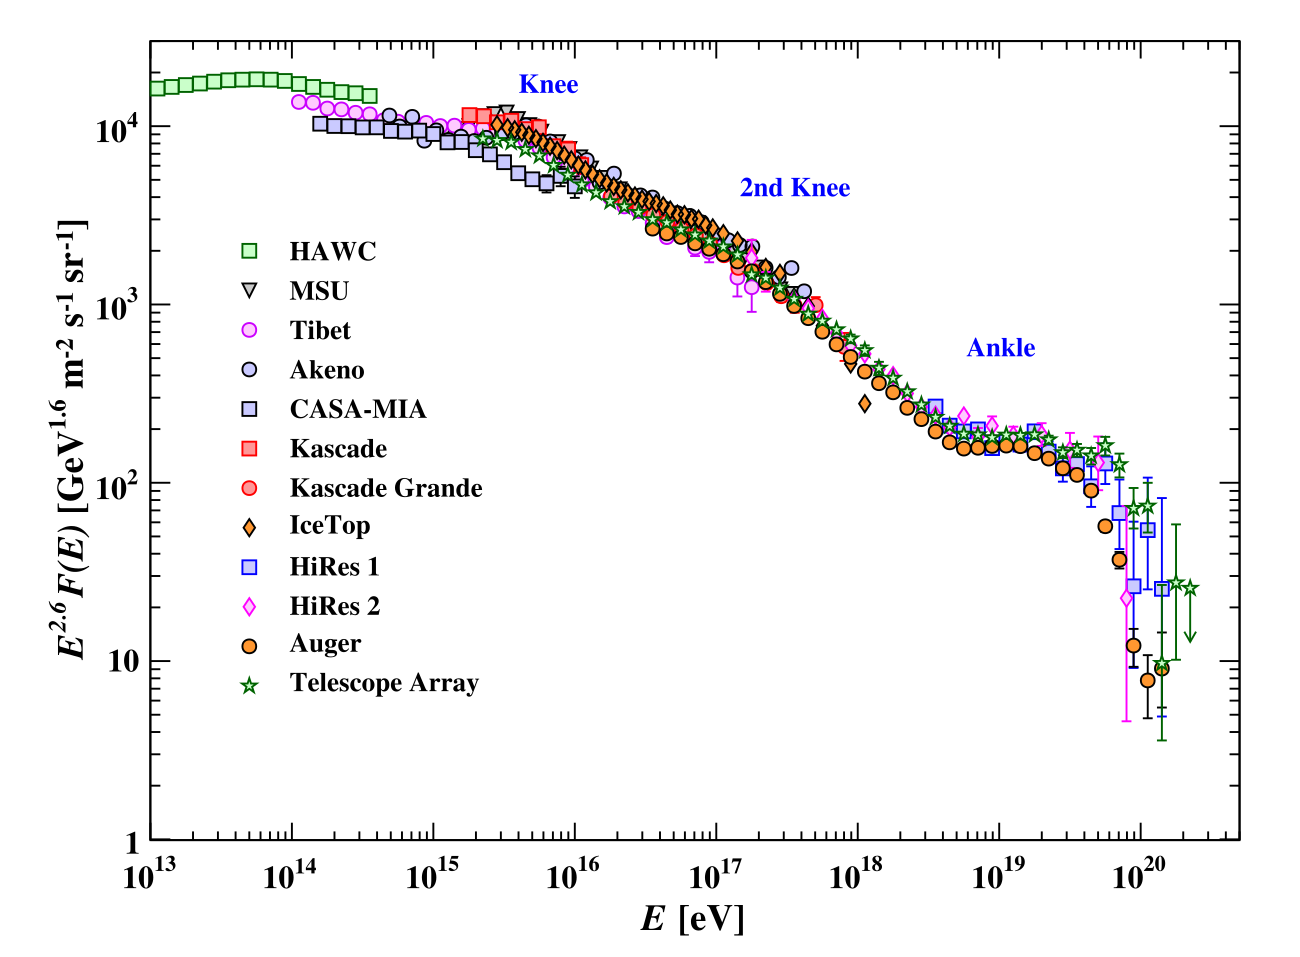
\includegraphics[width=0.8\textwidth]{figs/CR_Spectrum.png}
\caption{A plot of the cosmic ray spectrum assembled from observations from a variety of experiments. Major features visible are the knee ($\approx 10^{16} $ eV), and the ankle ($\approx 10^{19}$ eV). ~\cite{AustinThesis} }
\label{fig:CRSpectrum}
\end{figure}

\subsection{Acceleration Mechanism}
Though the exact origin of cosmic rays is still unknown, we can infer how these particles are being accelerated based on our knowledge of how charged particles behave. 
\begin{figure}[h]
\centering
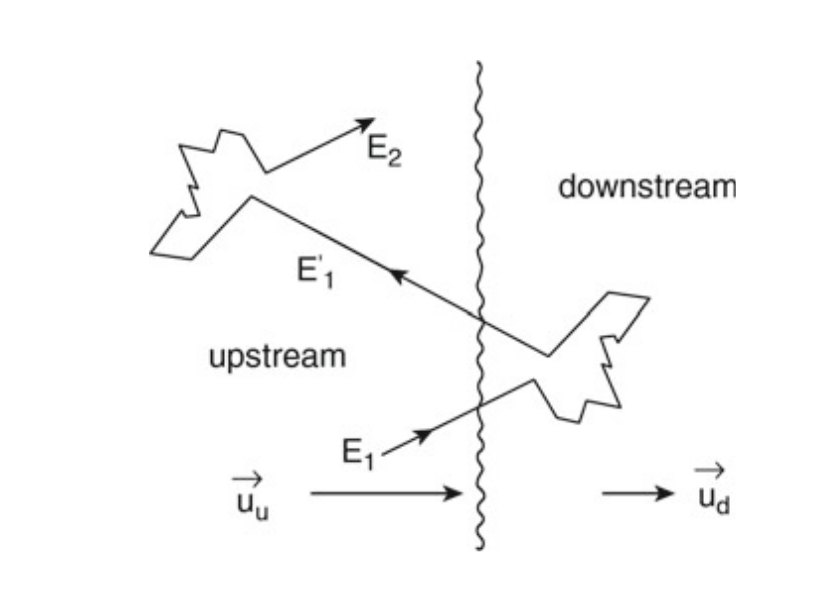
\includegraphics[width=0.8\textwidth]{figs/FermiFig.png}
\caption{Fermi acceleration of a plane shock front\cite{pimenta_partphys}. }
\label{fig:fermifig}
\end{figure}

Suppose a particle encounters a moving cloud of plasma. If it is large enough, the cloud will act as a massive scatterer. The overal collision is the result of a large number of individual scatterings inside the cloud, and the outgoing angle of the original particle is essentially random. On average the energy of the particle after a collision with this boundary will increase by a factor (eq.~\ref{secondfermieq}):

\begin{equation}
    \langle\frac{\Delta E}{E}\rangle \approx \frac{4}{3}\beta^2
\label{secondfermieq}
\end{equation}

Where $\beta=V/c$, corresponding to the boundary velocity. This is \textit{second order Fermi acceleration}, and is generally insufficient to explain the cosmic ray spectrum. If we instead assume a plane shock front, as in figure \ref{fig:fermifig} , then the post-collision velocity of the particle is no longer randomly distributed, and we instead obtain the expression (eq.~\ref{firstfermieq}):

\begin{equation}
    \langle\frac{\Delta E}{E}\rangle \approx \frac{4}{3}\beta
\label{firstfermieq}
\end{equation}

This describes \textit{first order Fermi acceleration}. From here, we can calculate the expected flux measured at Earth to be (eq.~\ref{fermiexpflux}):

\begin{equation}
    \frac{dN}{dE} \propto (\frac{E}{E_0})^{-\Gamma}
\label{fermiexpflux}
\end{equation}

where $\Gamma=\alpha+1$, $\alpha\approx \frac{3P_e}{4 \beta}$, and $P_e$ is the probability that a particle may escape the shock region (proportional to the velocity, $V$). Note that this is a power law with almost constant spectral index, as both $\beta$ and $P_e$ are proportional to $V$, similar to what is seen in the observed cosmic ray spectrum~\cite{pimenta_partphys}. 

We can additionally derive constraints on the maximum energy to which a particle can be accelerated based off the magnetic field intensity, $B$, and the size of the accelerating region, $R$ (eq.~\ref{HillasCond}):

\begin{equation}
    E_{max} = eBR \approx 10^{21} [\frac{R}{\textrm{1 pc}}][\frac{B}{\textrm{1 Gauss}}] \textrm{ eV}
\label{HillasCond}
\end{equation}

This is known as \textit{Hillas' condition}, and can inform us about the properties of cosmic ray accelerators. We can plot this condition to show sources which satisfy this requirement for a particular energy, producing what is commonly referred to as Hillas' plot (Figure \ref{fig:hillasplot}). Sources must exist above the diagonal thresholds in order to be valid accelerators of cosmic rays of certain energies. For example, sources capable of accelerating protons to ~100 EeV energies must exist above the dashed line in figure~\ref{fig:hillasplot}. Sources below are either too small, or have magenetic fields that are too weak.    

\begin{figure}[h]
\centering
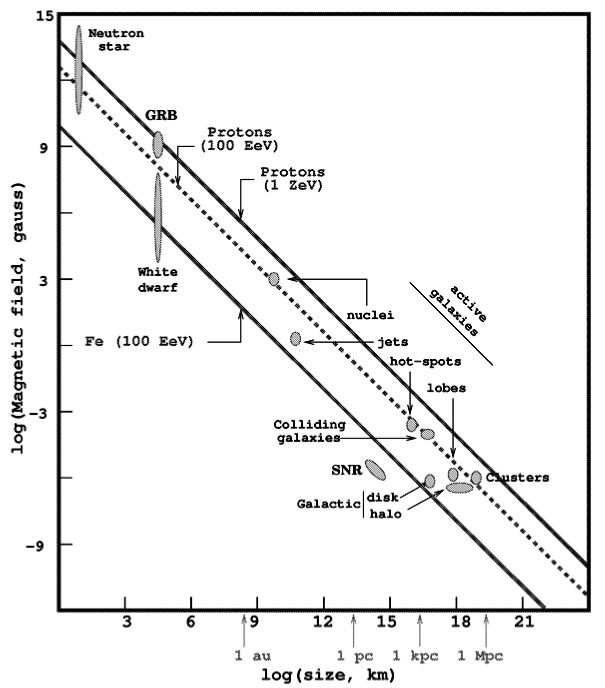
\includegraphics[width=0.8\textwidth]{figs/HillasPlot.jpg}
\caption{A Hillas plot, showing source populations capable of accelerating cosmic rays to a given energy, given their size and magnetic field strength~\cite{hillasplotsrc}.}
\label{fig:hillasplot}
\end{figure}


\section{Photons}
Perhaps the oldest and most well-studied astrophysical messenger, photons have the useful property of being electrically neutral. Unlike cosmic rays, their paths are not bent by magnetic fields, and the arrival directions of photons can be used to identify their origin, particularly at high energies due to their good angular resolution. Photons additionally span a large energy range, and can be used to explore a wide variety of astrophysical production processes. For the purposes of this work, we are most interested in the highest energy photons (gamma rays, with energies greater than 100 keV), which can be produced through either leptonic or hadronic processes.

\subsection{Leptonic Radiative Processes}
While photons cannot be directly accelerated by electric and magnetic fields, there are a variety of mechanisms by which processes involving leptons can produce high energy photons. 

\begin{itemize}
    \item \textbf{Synchrotron radiation:} Radially accelerated relativistic particles will release synchrotron radiation. This typically occurs as charged particles (such as electrons) spiral through magnetic fields. The power loss, ($dE/dT)$, due to synchrotron radiation for a particle of mass M and charge Z can be expressed as (eq. \ref{syncheq}):
    \begin{equation}
        -\frac{dE}{dT} \approx 2.6 (\frac{Zm_e}{M})^4(\frac{E}{\textrm{1 keV}})^2(\frac{B}{1\textrm{ G}})^2 \textrm{ keV s}^{-1}
    \label{syncheq}
    \end{equation}
    Where $m_e$ is the electron mass, $E$ is the particle energy, and $B$ is the magnetic field strength. From equation~\ref{syncheq} it can be seen that synchrotron emission is significantly more relevant for electrons than protons, due to the $1/M^4$ term.
    
    \item \textbf{Compton Scattering and Inverse Compton Scattering:} Photons may scatter off an electron at rest, and in doing so experience a wavelength shift according to (\ref{compeq}):
    \begin{equation}
        \frac{\lambda'-\lambda}{\lambda}=\frac{\hbar\omega}{m_e c^2}(1 - \cos\alpha)
    \label{compeq}
    \end{equation}
    Where $\lambda'$ and $\lambda$ correspond to the final and initial photon wavelengths, and $\alpha$ is the deflection angle of the photon. If a low energy photon collides with a high energy electron, the energy of the photon may exit with more energy than it began with, providing an effective mechanism for increasing the photon energy. 
\end{itemize}

A combination of these two processes can produce the two peak structure typically seen in the spectrum of observed gamma ray sources. The lower energy peak is due to synchrotron radiation, while the higher energy peak corresponds to low energy photons being scattered to higher energies via inverse compton scattering. 
    
\begin{figure}[h]
\centering
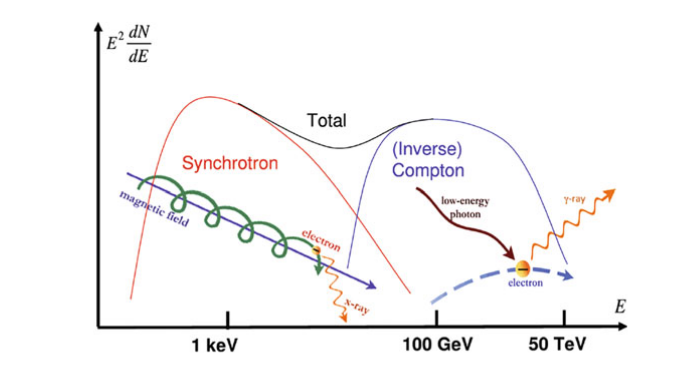
\includegraphics[width=0.8\textwidth]{figs/toygammaspect.png}
\caption{A cartoon plot of the gamma ray spectrum for a high energy gamma ray source. The two peak structure arises from the two production mechanisms of gamma rays. At lower energies, photons are produced by synchrotron radiation of electrons spiraling around magnetic field lines. The higher energy peak is then formed by the lower energy photons being scattered off energetic electrons via inverse compton scattering~\cite{pimenta_partphys_compton}. }
\label{fig:fermifig}
\end{figure}

\subsection{Hadronic Radiative Processes}
While leptonic processes can produce high energy gamma rays, hadronic processes will produce gamma rays in addition to neutrinos and cosmic rays. Protons accelerated to high energies in an astrophysical source may interact with other protons via (eq. \ref{hadeq}):

\begin{equation}
    p + p \rightarrow [\pi^0 + \pi^+ + \pi^-] + X
\label{hadeq}    
\end{equation}

Where X is the appropriate nucleus or hadron depending on the pions produced, and on average there is expected to be equal production of neutral and charged pions. Additionally, protons may interact with photons, providing an additional path to pion production (eq. \ref{hadeq2} and \ref{hadeq3}):

\begin{equation}
    p + \gamma \rightarrow \Delta^+ \rightarrow \pi^0 + p
\label{hadeq2}    
\end{equation}
\begin{equation}
    p + \gamma \rightarrow \Delta^+ \rightarrow \pi^+ + n
\label{hadeq3}    
\end{equation}

These resultant pions can subsequently decay, producing child particles depending on the particular pion type. Neutral pions will decay into gamma rays ($\pi^0 \rightarrow \gamma + \gamma$), and charged pions will decay to a lepton and their associated (anti)neutrino (most often muons and muon neutrinos: $\pi^+ \rightarrow \nu_{\mu} + \mu^+$, $\pi^- \rightarrow \bar{\nu_{\mu}} + \mu^-$). As such the sources of cosmic rays are expected to additionally produce a high energy gamma ray flux.

\subsection{Gamma Rays as an Astrophysical Messenger}
Gamma rays are a robust astrophysical messenger. As previously mentioned, photons are uncharged and their arrival directions can consequently be used to identify their origin. Additionally, the gamma ray energy can be used to infer information about the primary particle energy for a known production mechanism. Gamma rays are also well studied, and modern detectors boast high event rates: Fermi-LAT, for example, observes enough events to be capable of studying the temporal variability of sources on the timescale of approximately a day. 

Gamma rays are not without their limitations, however. Note that while at the highest energies gamma rays may be produced by both leptonic and hadronic processes, only hadronic processes are expected to additionally produce neutrinos and cosmic rays. For this reason, high energy gamma rays alone cannot be used to identify the source of high energy cosmic rays. 

Additionally, high energy gamma rays may also interact electromagnetically with the ambient radiation in the universe, undergoing pair production (eq. \ref{ppeq}):

\begin{equation}
    \gamma_{VHE} + \gamma_{CMB} \rightarrow e^+ + e^-
\label{ppeq}
\end{equation}

This interaction can occur between high energy gamma rays and photons from the CMB, leading to an event horizon for gamma rays of a particular energy. Figure \ref{fig:photeh} shows this horizon as a function of distance and photon energy. The photon event horizon prevents us from studying the highest energy photons from many AGN, and there is a significant region of parameter space below the highest observed cosmic ray energy that cannot be examined with photons alone. 

\begin{figure}[h]
\centering
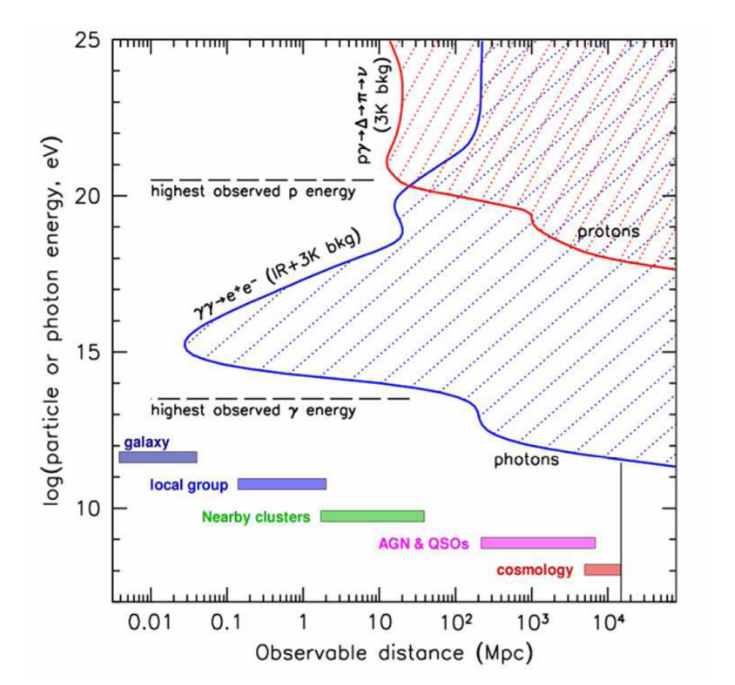
\includegraphics[width=0.8\textwidth]{figs/photevthorizon.png}
\caption{A plot of the photon and cosmic ray event horizons, showing the regions/energy scales visible using observations originating from photons (blue) and cosmic rays (red). Pair production of high energy photons with the ambient radiation in the universe prevents photon observations at long distances and high energies, including much of the energy scale below the highest observed cosmic ray energy. Also note that the photon event horizon can prevent us from studying the highest energy photons from AGN~\cite{Yuan_2011}. }
\label{fig:photeh}
\end{figure}

\section{Neutrinos}

\subsection{Production Mechanisms}
Neutrinos in astrophysical sources are produced via charged pion decay from pions produced from cosmic ray interactions with either photons or protons. The charge of the pion determines whether more neutrinos or anti-neutrinos are produced (eq. \ref{nuprodeq1} and \ref{nuprodeq2}):

\begin{equation}
    \pi^+ \rightarrow \nu_{\mu} + \mu^+ \rightarrow \nu_{\mu} + e^+ + \nu_{e}+\bar{\nu_{\mu}}
\label{nuprodeq1}
\end{equation}

\begin{equation}
    \pi^- \rightarrow \nu_{\mu} + \mu^- \rightarrow \bar{\nu_{\mu}} + e ^- + \bar{\nu_{e}}+\nu_{\mu}
\label{nuprodeq2}
\end{equation}

In either case, note that the expected flavor ratio of the neutrinos and anti-neutrinos produced at the source is $\nu_e : \nu_{\mu} : \nu_{\tau} = 1 : 2 : 0$. Combining this initial flavor ratio with neutrino oscillations over cosmic distances produces an expected observed astrophysical neutrino flavor ratio of $\nu_e : \nu_{\mu} : \nu_{\tau} = 1 : 1 : 1$.

Neutrinos are also produced by cosmic rays interacting with the Earth's atmosphere. This is referred to as the atmospheric neutrino flux, and has contributions both from pion decay ($\pi^+ \rightarrow \nu_{\mu} + \mu^+$, $\pi^- \rightarrow \bar{\nu_{\mu}} + \mu^-$), as well as kaon decay ($K^0_L \rightarrow \pi^\pm+ e^\mp +\nu_e$, $K^0_L \rightarrow \pi^\pm+ \mu^\mp +\nu_\mu$, $K^+ \rightarrow \mu^+ +\nu_\mu$, $K^+ \rightarrow \pi^0 + e^+ +\nu_e$, $K^+ \rightarrow \pi^0 + \mu^+ +\nu_\mu$). Below 100 TeV, the resultant spectrum closely follows that of cosmic rays, with a spectral index of $\gamma_{atmos}=2.7$. At higher energies the shower mesons are able to travel further in the atmosphere, giving them an increased opportunity to interact and steepening the spectral index to $\gamma_{atmos}=3.7$. The atmospheric neutrino flux exists as an irreducible background for many studies of the origin of astrophysical neutrinos. 

\subsection{Observed Neutrino Spectrum}
Both the astrophysical and atmospheric neutrino fluxes have been observed in data from the IceCube detector, with the astorphysical neutrino spectral index being measured to be $\gamma_{astro} \approx 2.28$ \cite{stettner2019measurement}.  While astrophysical and atmospheric neutrinos are largely indistinguishable on an individual event basis, the difference in spectra between the two populations ($\gamma_{astro} \approx 2.28$, $\gamma_{atmos} \approx 3.7$) allows us to distinguish between the two on a statistical basis. Higher energy events are more likely to be astrophysical in origin, and an equal share of astrophysical and atmospheric neutrinos can be expected at $\approx$ 200 TeV. Currently, the source(s) of the astrophysical neutrino flux have yet to be identified. For this reason, the observed astrophysical neutrino flux is commonly referred to as the "diffuse" astrophysical neutrino flux (as opposed to a "point source" flux, where specific astrophysical objects that are producing neutrino are identified).

\begin{figure}[h]
\centering
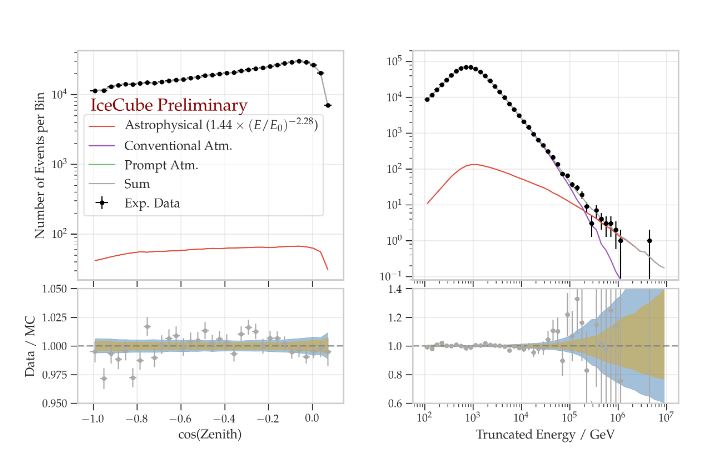
\includegraphics[width=0.8\textwidth]{figs/northerntracks_diffusefit.png}
\caption{Observation of the astrophysical neutrino flux in through-going tracks detected by the IceCube Neutrino Observatory. The effect is most visible in the plot of the observed energy spectrum on the right, showing the atmospheric contribution (blue) and the astrophysical contribution (red). The excess of events at high energies is unable to be explained without including a non-zero astrophysical contribution~\cite{stettner2019measurement}. }
\label{fig:diffusefit}
\end{figure}

\subsection{Neutrinos as Astrophysical Messengers}
As noted in the previous section, hadronic processes in astrophysical sources can produce neutrinos via pion decay. Like gamma rays, neutrinos are electrically neutral, and thus their paths are not bent by magnetic fields. Unlike gamma rays, however, neutrinos do not interact electromagnetically, instead interacting only via the weak force. Because of this, the mean free path of neutrinos traveling through the universe is significantly greater than that of photons, allowing us to use neutrinos to probe regions normally opaque to gamma rays. 

Astrophysical neutrinos are not without their drawbacks, however. The fact that neutrinos interact only weakly necessitates the construction of large detectors in order to observe an appreciable number of astrophysical events. Such detectors also observe a large, irreducible background of atmospheric neutrinos, particularly at lower (TeV) energies. For this reason, multi-messenger approaches that combine information from neutrinos and other astrophysical messengers are commonly used to attempt to identify the sources of astrophysical neutrinos. 


\subsection{AGN as Neutrino Source Candidates}
Since neutrinos can be used as an indicator of hadronic processes in astrophysical sources, identifying the source of the astrophysical neutrino flux is a promising route to also identifying the source of ultra-high energy cosmic rays. Though the source of the astrophysical neutrino flux has yet to be fully determined, in recent years there have been promising hints that extragalactic AGN are at least partially responsible.

An active galactic nucleus (AGN) is a compact region at the center of a galaxy displaying elevated electromagnetic emission, such that the additional luminosity cannot be attributed to stars. The luminosity is expected to originate from the accretion disk surrounding a supermassive black hole at the center of the galaxy, where conditions are thought to be ideal for high-energy particle acceleration and production.

The angle at which the AGN is viewed relative to its jet determines its exact classification, as can be seen in figure \ref{fig:AGNfig}. If the AGN is viewed "down" the jet (i.e. the jet is directed at Earth), the AGN is seen to be particularly luminous and is referred to as a blazar. Blazars can be further divided into two subclasses: flat spectrum radio quasars (FSRQ), which have luminous broad emission lines and continuous thermal emission, and BL-Lacs, which have weak or absent broad emission lines. AGN viewed off-axis fall into a variety of other classifications, with further sub-classification being defined by the spectrum of the AGN in various wavelength bands.

\begin{figure}[h]
\centering
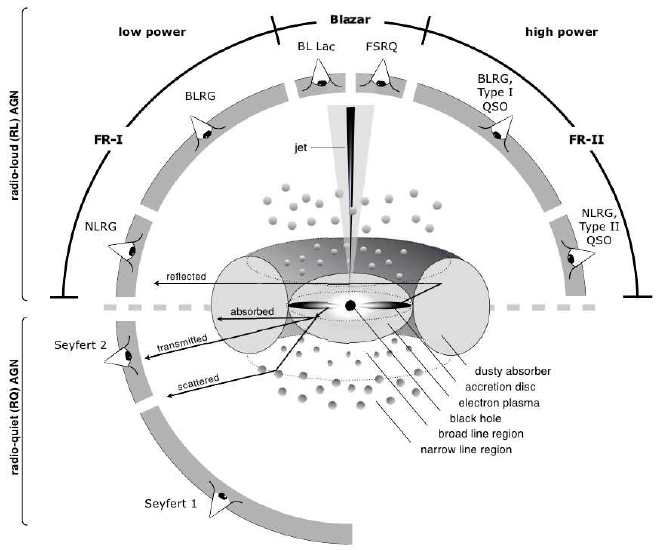
\includegraphics[width=0.8\textwidth]{figs/AGNfig.png}
\caption{The unified AGN model, showing the various classifications of AGN for different observation angles. If the jet is directed at Earth, the object is viewed as a blazar, while other viewing angles can obscure the jet, leading to alternative classification (e.g. as a Seyfert galaxy)~\cite{AGN_model_src}. }
\label{fig:AGNfig}
\end{figure}

\subsubsection{TXS 0506+056}
On September 22, 2017, the IceCube Neutrino Observatory detected a high energy neutrino, IceCube-170922A, with an energy of approximately 290 TeV. The arrival direction of IceCube-170922A was consistent with the location of the blazar TXS 0506+056, and sparked multi-messenger followup from a variety of other telescopes and detectors. Notably, it was determined that TXS 0506+056 was flaring in gamma rays at the time IC-170922A was observed. The significance of the positional correlation of a high energy IceCube event and a flaring blazar was calculated to be $3.0 \sigma$, providing the first hint that blazars may be a source of high energy astrophysical neutrinos~\cite{TXS_Multimessenger}.

\begin{figure}[h]
\centering
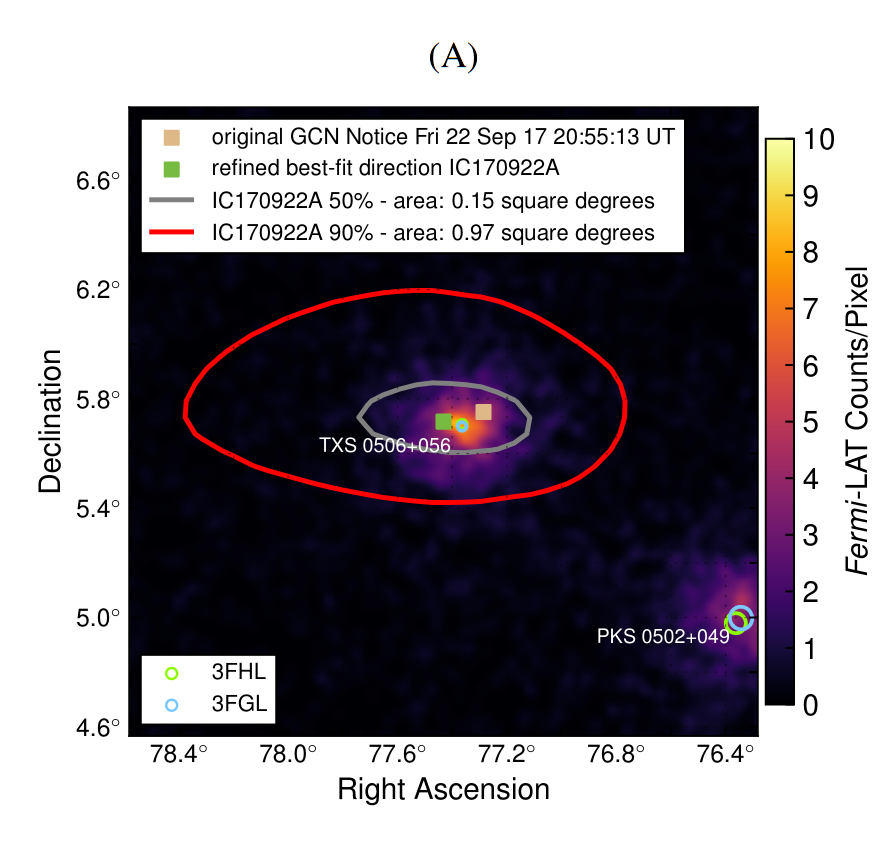
\includegraphics[width=0.8\textwidth]{figs/FermiMap.png}
\caption{The Fermi-LAT skymap near the location of the observed high energy IceCube event IC170922A, with the 50\% and 90\% error contours associated with IC170922A plotted in grey and red, respectively. The significance associated with the spatial coincidence of the high energy event and TXS 0506+056 was found to be $3.0 \sigma$~\cite{TXS_Multimessenger}. }
\label{fig:FermiMap}
\end{figure}

In addition to examining the multi-messenger correlation of a high energy IceCube event and a flaring blazar, an analysis of archival IceCube data was performed at the coordinates of IC170922A, examining the historical behavior of neutrino emission from this location of the sky over the previous nine years. In addition to the original high energy event observed in 2017, this archival analysis also revealed a 158 day period of elevated neutrino emission beginning in September 2014. The significance of this archival "neutrino flare" was calculated to be $3.5\sigma$. Unlike the 2017 high energy event, the 2014 neutrino flare did not correspond to a flaring period for TXS 0506+056 in gamma rays.~\cite{TXS_Archival}

\begin{figure}[h]
\centering
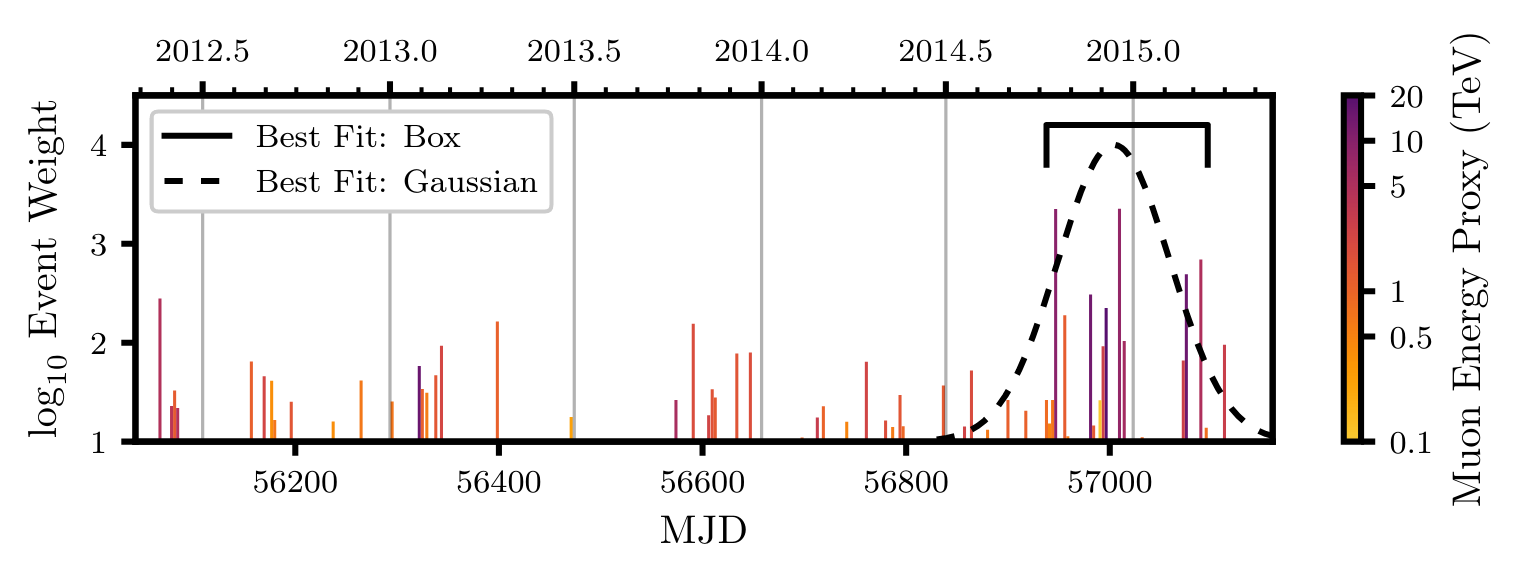
\includegraphics[width=0.8\textwidth]{figs/TXS_flarecurve.png}
\caption{The result of the archival analysis of IceCube data near the location of TXS 0506+056, with the $3.5\sigma$ flare shown. This flare is separate from the high energy event observed in 2017, and there was no corresponding flare observed in gamma rays during this time period~\cite{TXS_Archival}. }
\label{fig:TXS_flarecurve}
\end{figure}

The combination of a $3.0 \sigma$ multimessenger result with the $3.5 \sigma$ "untriggered" neutrino flare in 2014 suggest a significance of TXS 0506+056 as a neutrino source of at least $3 \sigma$. This makes for a strong argument for extragalactic blazars as interesting source candidates from the perspective of neutrino astronomy. 

\subsubsection{NGC 1068}
In addition to the multimessenger and archival results associated with TXS 0506+056, the results of the 10-year time integrated IceCube analysis~\cite{10yr_tint} also seem to suggest AGN as candidates for astrophysical neutrino emission. In this all-sky, untriggered, time integrated analysis, the most significant point in the northern sky appears to be spatially coincident with the Seyfert II galaxy NGC 1068. Notably, NGC 1068 was also included in an associated time integrated catalog analysis. In this catalog analysis, the pre-trial significance of time-integrated neutrino emission from NGC 1068 was $1.8 \times 10^{-5}$, corresponding to a significance of $2.9\sigma$. At a 14.4 Mpc distance, NGC 1068 is the most luminous Seyfert II galaxy detected by Fermi-LAT, and NGC 1068 had additionally been hypothesized as a candidate cosmic ray accelerator prior to this particular analysis\ \cite{NCG_1}\cite{NGC_2}\cite{NGC_3}.

It should additionally be noted that the catalog analysis mentioned above identified three other objects which, together with NGC 1068, collectively form a $3.3\sigma$ excess over the background expectation. These objects are the Seyfert II galaxy NGC 1068, the blazar TXS 0506+056,and the BL Lacs PKS 1424+240 and GB6 J1542+6129 \cite{10yr_tint}, providing further indication of AGN as potential neutrino emitters. 

\begin{figure}[h]
\centering
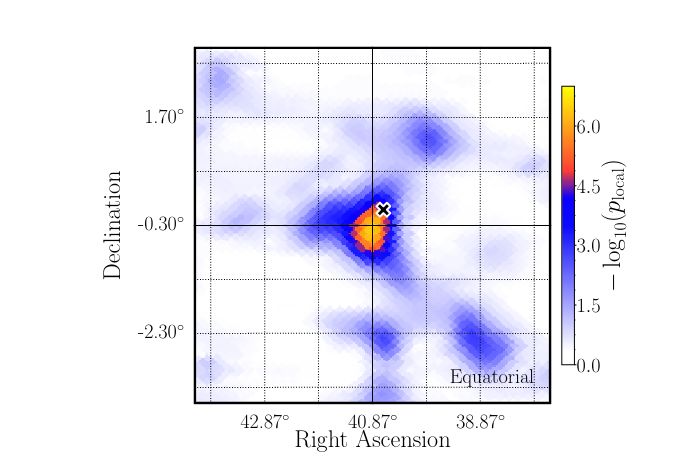
\includegraphics[width=0.8\textwidth]{figs/NGC_tint.png}
\caption{The results of the untriggered time integrated IceCube point source search analysis, showing the most significant spot in the northern sky, with the location of NGC 1068 plotted as the black "X"~\cite{10yr_tint}. }
\label{fig:NGC_tint}
\end{figure}


\subsection{Galactic Neutrino Sources}
Though this work will primarily focus on searches for extra-galactic point sources of the astrophysical neutrino flux, potential neutrino emission from sources within our galaxy is an active area of study as well. Notably, one of the first confirmed sources of lower energy astrophysical neutrinos was Supernova 1987A \cite{Bionta:1987qt}, a supernova occurring within the Milky Way. Other galactic objects that are considered candidates for neutrino emission include supernova remnants \cite{snr_2020}, as well as pulsar wind nebula \cite{pwn_2020}, both of which are known to produce gamma rays. 

The majority of the galactic plane lies in the southern sky. Since neutrino telescopes make use of the earth to block out atmospheric muon backgrounds (see subsequent chapter), this means that to best study the galactic plane, a neutrino observatory located in the northern hemisphere would be required. While there are several such telescopes either planned or under construction \cite{Agostini_2020}\cite{kappes2007km3net}, they have yet to reach effective volumes comparable to the existing IceCube observatory (located in the southern hemisphere). 

\subsection{Constraints on Neutrino Source Populations from Diffuse Measurements}
It is important to keep in mind that whatever the sources of astrophysical neutrinos may be, they must combine to reproduce the measured diffuse astrophysical neutrino flux. The current best fit astrophysical neutrino spectrum, assuming a single power law in energy, is given as (eq. \ref{diffuse_fit}):

\begin{equation}
    \frac{d\phi_{\nu+\bar{\nu}}}{dE} = 1.44_{-0.24}^{+0.25} (\frac{E}{100 \textrm{TeV}})^{-2.28_{-0.09}^{+0.08}} 10^{-18} \textrm{GeV}^{-1}\textrm{cm}^{-1}\textrm{s}^{-1}\textrm{sr}^{-1}
\label{diffuse_fit}
\end{equation}

This places constraints on the density and luminosity of potential astrophysical neutrino source populations. If a candidate source population has sources that are too numerous and/or too bright, then that source population would produce a higher flux of astrophysical neutrinos than has been observed, and an explanation of the nondetection of the additional flux is required. Similarly, if sources are too sparse and/or too dim, then such a source class is incapable of explaining the entirety of the measured diffuse flux. 

These constraints can be summarized in figure \ref{fig:muraseplot}, showing the band of the measured diffuse flux in source density/luminosity space, as well as several commonly discussed source populations. It should be noted that in this plot, the luminosity values for various source populations are derived from the electromagnetic luminosity $L_\gamma$. In principle, the true ratio $L_\nu/L_\gamma$ remains unknown, and consequently the positions of sources along the luminosity axis may shift according to this value. 


\begin{figure}[h]
\centering
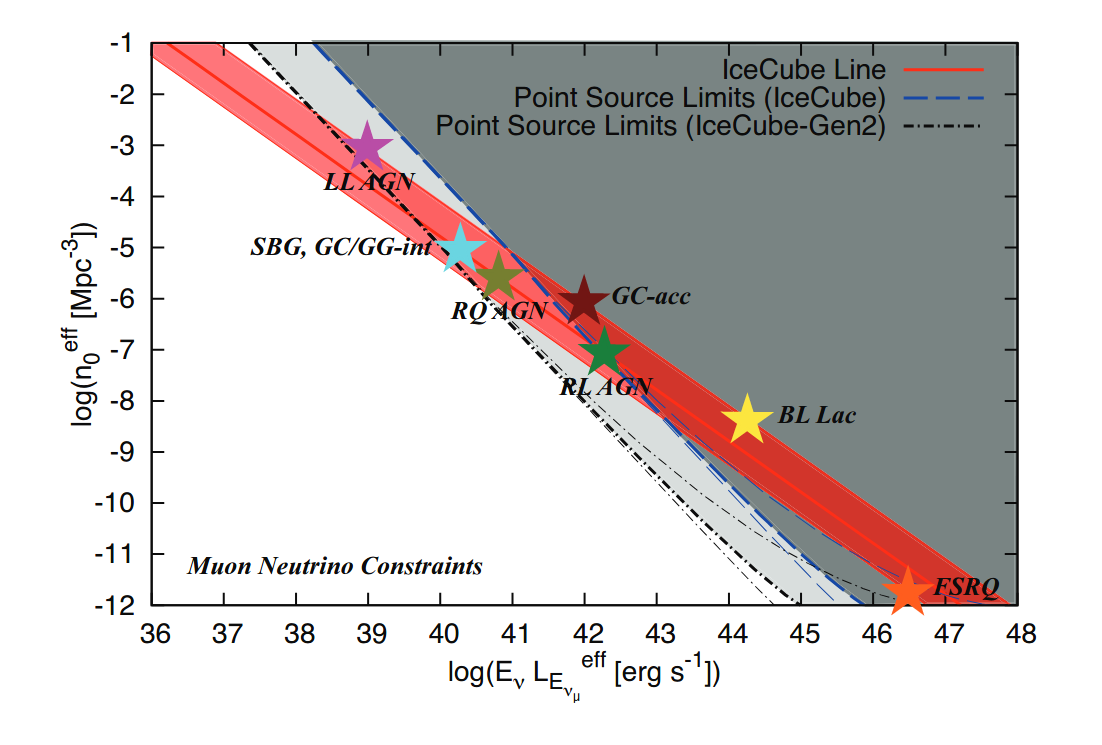
\includegraphics[width=0.8\textwidth]{figs/muraseplot.png}
\caption{Constraints on potential populations of sources of the high energy astrophysical neutrino flux. The red band represents combinations of source density and luminosity that are consistent with the measured astrophysical neutrino flux. Source populations that lie above this band are too bright and/or too numerous, while source below this band are too dim/too sparse. Also shown are limits derived from the non-observation of neutrino sources in time-integrated analyses performed by the IceCube collaboration as of 2016, as well as a projected set of limits that would be associated with a non-observation from IceCube-Gen2~\cite{Murase_constraints}. }
\label{fig:muraseplot}
\end{figure}


\chapter{The IceCube Detector}\label{chapter:icecubedetector}
The IceCube Detector is a large (cubic kilometer scale) water cherenkov detector situated underneath the ice at the south pole. Its large volume makes it ideal for studying high energy (TeV and higher) neutrino events originating from either the atmosphere or astrophysical sources. 

\section{Detection Mechanism}
The cross section for neutrino interaction in Earth can be seen in figure \ref{fig:cross_sections}. These cross sections are small, but the Earth is also quite large. We can calculate the mean free path for neutrinos traveling through Earth as (eq. \ref{mfp}):

\begin{equation}
    \lambda = \frac{1}{\sigma_{\nu}\rho_{Earth}}
    \label{mfp}
\end{equation}

Using the neutrino cross section near 1 PeV ($\sigma_{\nu} \approx 10^{-33}$ cm$^2$), and the density of the Earth ($\approx 5.5$ g/cm$^3$, corresponding to a nucleon density of $\rho_{Earth}=3.3 \times 10^{24}$ cm$^{-3}$), we obtain an estimate of the neutrino mean free path of $\approx 3000$ km. Since the diameter of the Earth is approximately $1.3 \times 10^4$ km, we can conclude that the Earth is opaque to high energy neutrinos. We can detect the neutrinos that interacted in the Earth by way of identifying their interaction products. 

For the purposes of neutrino point source searches, we primarily focus on neutrinos interacting either through charged current (CC) or neutral current (NC) interactions. In both cases, the energy of the neutrinos observed by the IceCube detector is high enough that neutrinos interact through deep inelastic scattering with nucleons in the antarctic ice. In neutral current (NC) interactions, the process is mediated by a neutral Z boson, as shown on the left in figure \ref{fig:nuinteractions}. In this case, the product of the interaction is a neutrino, meaning the only visible signature of this interaction is the production of a hadronic particle cascade. 

\begin{figure}[h]
\centering
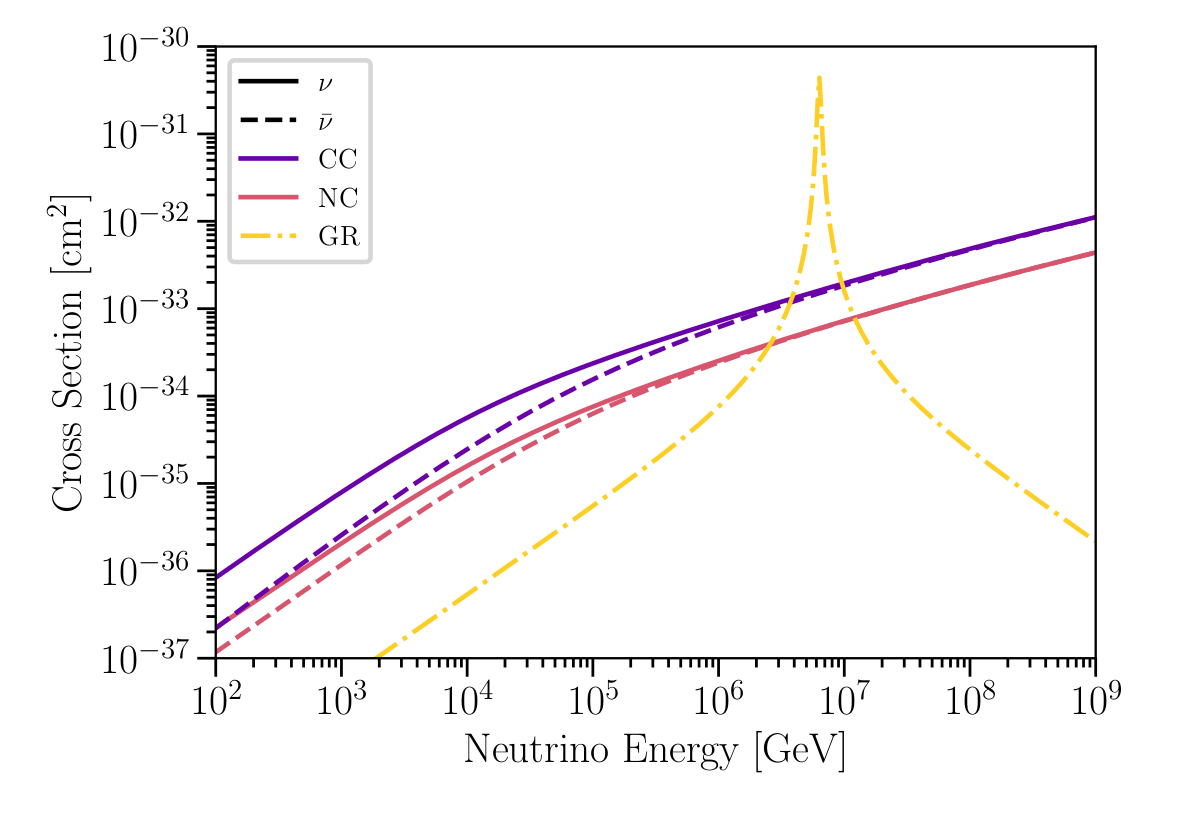
\includegraphics[width=0.8\textwidth]{figs/nu_cross_sections.png}
\caption{The cross sections of various neutrino interactions in the Earth. The yellow curve corresponds to Glashow Resonance \cite{IceCubeGlashow}, whereby an anti-electron neutrino combines with an atomic electron to produce a W+. These events are relatively rare in IceCube data, and are subsequently not used in the context of astrophysical neutrino source searches.}
\label{fig:cross_sections}
\end{figure}

Charged current interactions are mediated by a charged W boson, and can be summarized as (eq. \ref{ccinteraction1} and \ref{ccinteraction2}):

\begin{equation}
    \nu_\ell +  n \rightarrow \ell^- + p
\label{ccinteraction1}
\end{equation}
\begin{equation}
    \bar{\nu}_\ell +  p \rightarrow \ell^+ + n
\label{ccinteraction2}
\end{equation}

The Feynman diagrams for this process can be seen on the right in figure \ref{fig:nuinteractions}. Notably, charged current interactions produce an outgoing lepton $\ell^\plusminus$ in addition to a hadronic cascade. This is particularly useful in the case that the lepton produced is a muon, as muons can travel a sizeable distance (hundreds, or even thousands of meters) before decaying. If the lepton recieves enough energy, it will subsequently produce cherenkov radiation, as it will be traveling faster than the local speed of light in ice. This radiation is emitted at an angle $\theta_c$ relative to the direction of travel, where $\theta_c$ is given by (eq. \ref{cherenkoveq}):

\begin{equation}
    \cos(\theta_c) = \frac{1}{n\beta}
\label{cherenkoveq}
\end{equation}

Where $n$ is the index of refraction of the medium through which the particle is traveling (in this case ice), $\beta = \frac{v}{c}$, and $v$ is the velocity of the traveling particle (the lepton, in this case).  For ice, $n=1.31$, and this emission angle is approximately 41 degrees. The number of photons expected per unit track length is given by the Frank-Tamm formula \cite{FrankTamm} (eq. \ref{FrankTamm}):

\begin{equation}
    \frac{dN}{dxd\lambda} = \frac{2\pi z \alpha}{\lambda^2}\sin^2(\theta_c)
\label{FrankTamm}
\end{equation}

Where $z$ is the charge of the ionizing particle, $\lambda$ is the wavelength of the emitted radiation, $\alpha$ is the fine structure constant ($\approx \frac{1}{137}$), and $\theta_c$ is the cherenkov angle given by eq. \ref{cherenkoveq}. Peak emission is found in the optical portion of the light spectrum, between 350 and 600 nm corresponding to a characteristic blue hue. 

To summarize, neutrinos traveling through the antarctic ice will occasionally interact, producing child particles that will emit cherenkov radiation. We can then build an array of photon detectors to detect these photons, and subsequently infer information about the original incident particles. 

\begin{figure}[h]
\centering
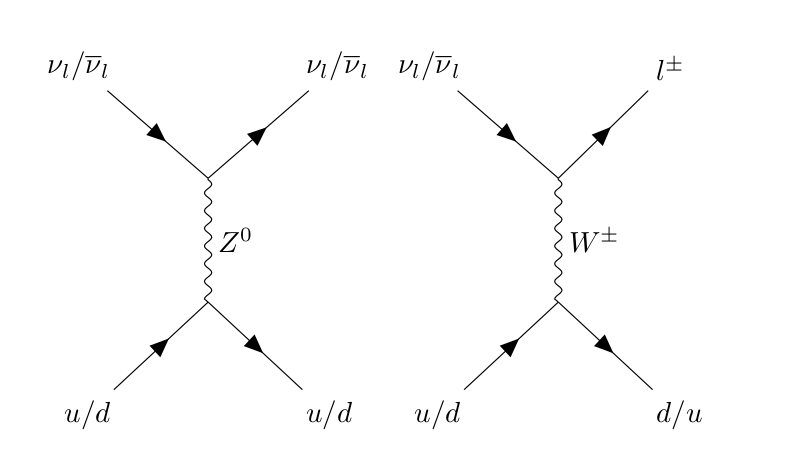
\includegraphics[width=0.8\textwidth]{figs/nuinteractions.png}
\caption{The Feynman diagrams corresponding to neutral current (left) and charged current (right) neutrino interactions. Charged current interactions can produce a detectable outgoing lepton in addition to a hadronic cascade, while neutral current interactions only produce a hadronic cascade.}
\label{fig:nuinteractions}
\end{figure}

\section{The Physical Components of the IceCube Detector}
As outlined in the previous section, the strategy for detecting neutrinos with a water cherenkov detector is not to directly detect the neutrinos themselves, but rather to detect the cherenkov photons from the outgoing particles resulting from the neutrino interactions. The IceCube detector accomplishes this through the use of a large number of photomultiplier tubes (PMTs). At the very highest level, a PMT is a device that converts photons to an electrical signal that can then be read out by a set of associated electronics. The details of general PMT design and operation can be found in \cite{tavernier_pmt}.

\begin{figure}[h]
\centering
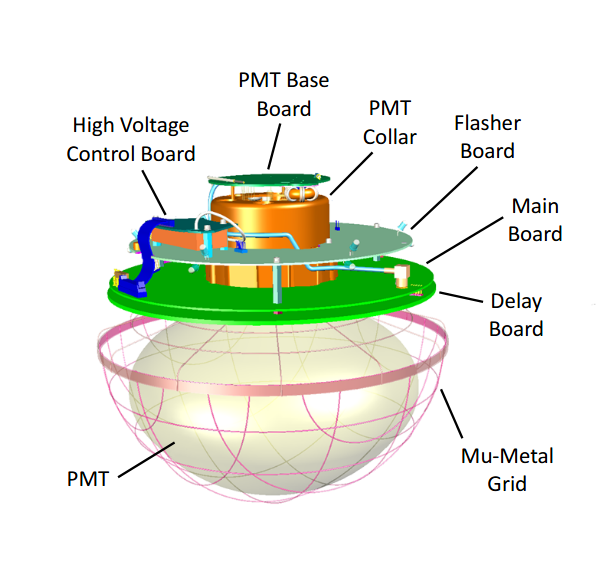
\includegraphics[width=0.8\textwidth]{figs/DOM.png}
\caption{A diagram of a single IceCube digital optical module (DOM). The entire apparatus is encased in a pressurized glass sphere for protection (not shown). The PMT faces downward for optimal collection of photons from upgoing neutrino events. In addition to the PMT, each DOM also contains digitization electronics and an array of LED flashers that can be used for calibration ~\cite{det_paper}. }
\label{fig:DOM}
\end{figure}

In IceCube, PMTs are housed in a single unit referred to as a digital optical module ("DOM"), seen in figure \ref{fig:DOM}. Each module contains the PMT and its associated electronics, as well as a set of LED flashers that can be used to calibrate the detector once the DOMs have been lowered into the ice. DOMs are arranged onto 86 vertical strings, 78 of which contain 60 DOMs spaced ~17 meters apart along the length of the string. These strings are arranged into a hexagonal grid pattern under the south pole ice with a separation between strings of approximately 125 meters, resulting in a cubic kilometer of instrumented ice extending between 1400 and 2400m below the surface of the south pole ice sheet. The remaining 8 strings form the DeepCore sub-array, a more densely instrumented region near the center of the detector, primarily used for studying lower ($\approx$100s of GeV) scale events. PMTs that are part of the DeepCore portion of the detector have a higher quantum efficiency than those on the other 78 strings \cite{deepcorepaper}.  

A diagram of the IceCube detector can be seen in figure \ref{fig:icecubediagram}. Due to the weakly interacting nature of neutrinos combined with a power law spectrum, a large detector volume is critical to detecting the astrophysical neutrino flux. Prior to IceCube's construction, calculations indicated that a cubic-kilometer scale detector would be necessary to observe an appreciable event rate of astrophysical neutrinos \cite{Halzen_2002}\cite{Waxman_1998}. The size and design of IceCube are well suited for detecting astrophysical neutrino events in the TeV+ energy range, as the large instrumented volume ensures a significant number of interactions in this energy range, and the detector's nanosecond scale timing resolution makes event reconstruction possible for events producing cherenkov radiation over the scale of $\approx$100s of meters. 

\begin{figure}[h]
\centering
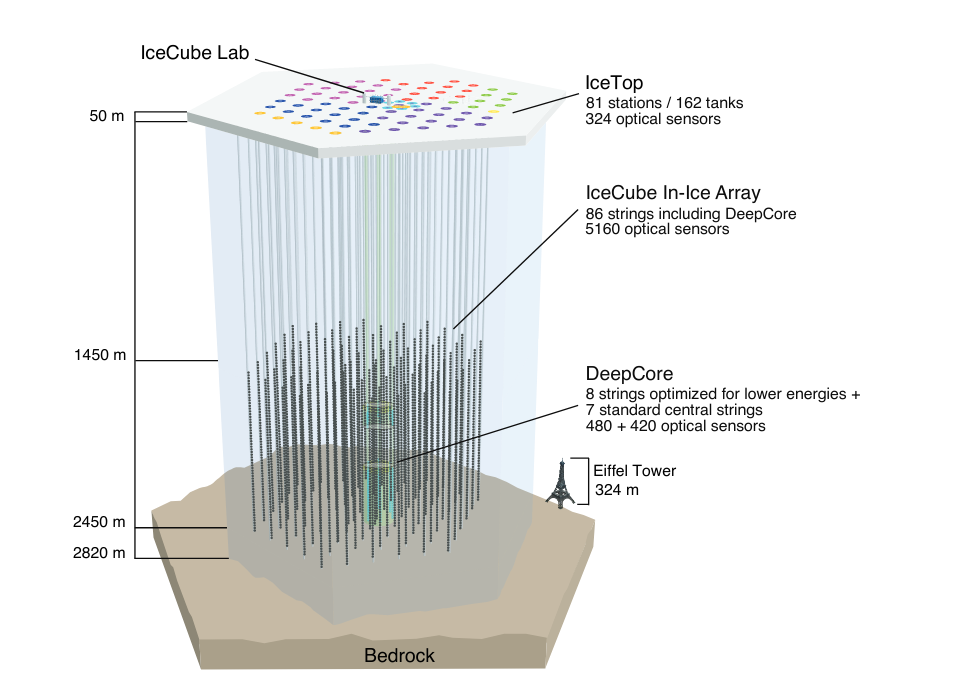
\includegraphics[width=0.8\textwidth]{figs/icdiagram.png}
\caption{A diagram of the IceCube detector. The detector consists of 86 strings of DOMs lowered into holes drilled in the pattern of a hexagonal grid defined by a separation of 125 meters. Each string is formed by 60 DOMs connected by a cable, used for powering the DOMs and communication with the IceCube Lab (ICL) on the surface. The instrumented detector volume begins at a depth of 1450 meters, and extends down to 2450 meters, resulting in approximately a cubic kilometer of instrumented ice~\cite{det_paper}. }
\label{fig:icecubediagram}
\end{figure}

As the IceCube detector is situated in the south pole ice, a proper description of the optical properties of the ice is key for being able to accurately reconstruct events. While the ice is generally clear, it does contain several impurities and features that make it optically nonuniform. The scattering and absorbtion of light are known to vary as a function of depth, as seen in figure \ref{fig:icedepth}. The large peak near a depth of 2000 meters is thought to correspond to a layer of dust deposited on the south pole ice sheet many years in the past, and is commonly referred to as "the dust layer" (physicists are not always the most creative with names). 

In addition to varying as function of depth, the optical properties of the ice also vary as a function of azimuth. The largest effects along this axis are the ice tilt and ice anisotropy. The ice tilt refers to the layers of ice with similar optical properties being not perfectly horizontal, and results in a variation in scattering and absorption as light travels in different directions through the ice sheet. The ice anisotropy is similar, but has an observed additional axis of symmetry, leading to variations that are twice as frequent as a function of azimuth. Notably, while this effect was original observed in calibration data using LED flashers, it is visible in data from observed atmospheric muons, as seen in figure \ref{fig:anisotropyplot}. 

The final major optical nonuniformity of the detector ice is the hole ice. During the construction of the IceCube detector, holes were drilled in the south pole ice, and strings of DOMs were lowered down the appropriate depth. The water in these holes then refroze with different optical properties than the surrounding ice. The column of refrozen ice is referred to as the "hole ice", typically containing an inner region where air bubbles have been trapped referred to as the "bubble column". The hole ice has significantly shorter scattering distances, and is an area of active study within the IceCube collaboration. 

\begin{figure}[h]
\centering
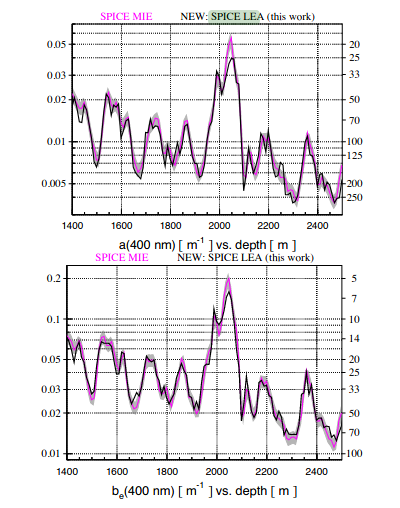
\includegraphics[width=0.8\textwidth]{figs/icedepth.png}
\caption{Plots of the scattering and aborption of light as a function of depth in the south pole ice. The peak near a depth of 2000 meters is referred to as "the dust layer", and is thought to correspond to a layer of dust deposited at the south pole at some point in the Earth's history.  ~\cite{iceproceedings} }
\label{fig:icedepth}
\end{figure}

\begin{figure}[h]
\centering
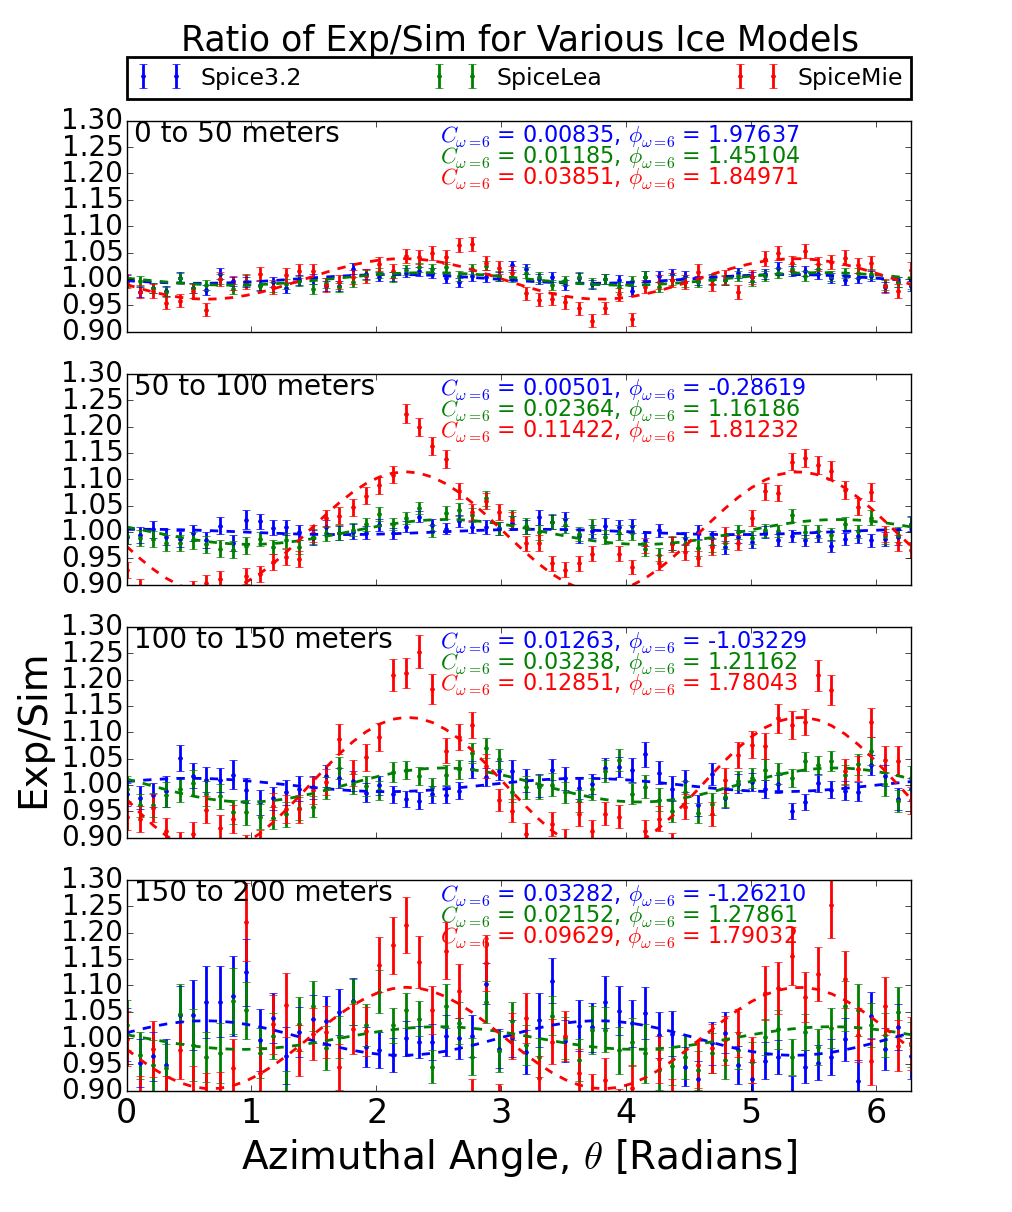
\includegraphics[width=0.8\textwidth]{figs/fourierfits.png}
\caption{Plots of the ratio of light seen from atmospheric muons in experiment and simulation using various ice models (SpiceMie, SpiceLea, and Spice3.2), as a function of azimuthal angle between the muon track and the observing DOM. SpiceMie does not account for the ice anisotropy, resulting in a sinusoidal shape that grows with distance. SpiceLea and Spice3.2 both account for the anisotropy, and consequently the sinusoidal shape is reduced in amplitude when using these ice models.}
\label{fig:anisotropyplot}
\end{figure}

\section{Event Types}
IceCube events can be generally be categorized into three different types: tracks, cascades, and double cascades. While neutral current events exclusively correspond to cascades, charged current events can produce any of the three, dependent on the variety of the outgoing lepton. This gives IceCube the ability to identify the flavor of the incident neutrino, and this fact can be leveraged to do a large amount of interesting physics. However, for the purposes of this work, we are primarily interested in tracks, due to their excellent pointing resolution as discussed below. 

\subsection{Tracks}
From equation \ref{ccinteraction1} we can see that charged current interactions produce an outgoing lepton, which will in turn produce cherenkov radiation if it is energetic enough. In particular, if the outgoing particle is a muon, it will travel a significant distance before decaying or exiting the detector. As the muon produces cherenkov radiation as it travels through the ice, the pattern of DOMs which detect this radiation will resemble a line, as shown in figure \ref{fig:evttypes}. These events are referred to as "tracks". If the neutrino interaction occurred inside the IceCube detector, then the track will appear to start within the detector, and the event can be referred to as a "starting track". If instead the neutrino interaction occurred outside the detector, and the resultant muon traveled through the detector, then the event is instead referred to as a "through-going track" (again, physicists are not the most creative). Through-going tracks can result from astrophysical neutrinos, as well as atmospheric neutrinos and atmospheric muons (muons resulting from cosmic ray interactions in the atmosphere). Starting tracks, however, can only be produced by muons originating from atmospheric or astrophysical neutrinos. For the purposes of this work, we will focus primarily on through-going tracks, however starting tracks are also scientifically interesting, and can be used for point-source and diffuse analyses of the neutrino flux as well \cite{Estes}.

\begin{figure}[h]
\centering
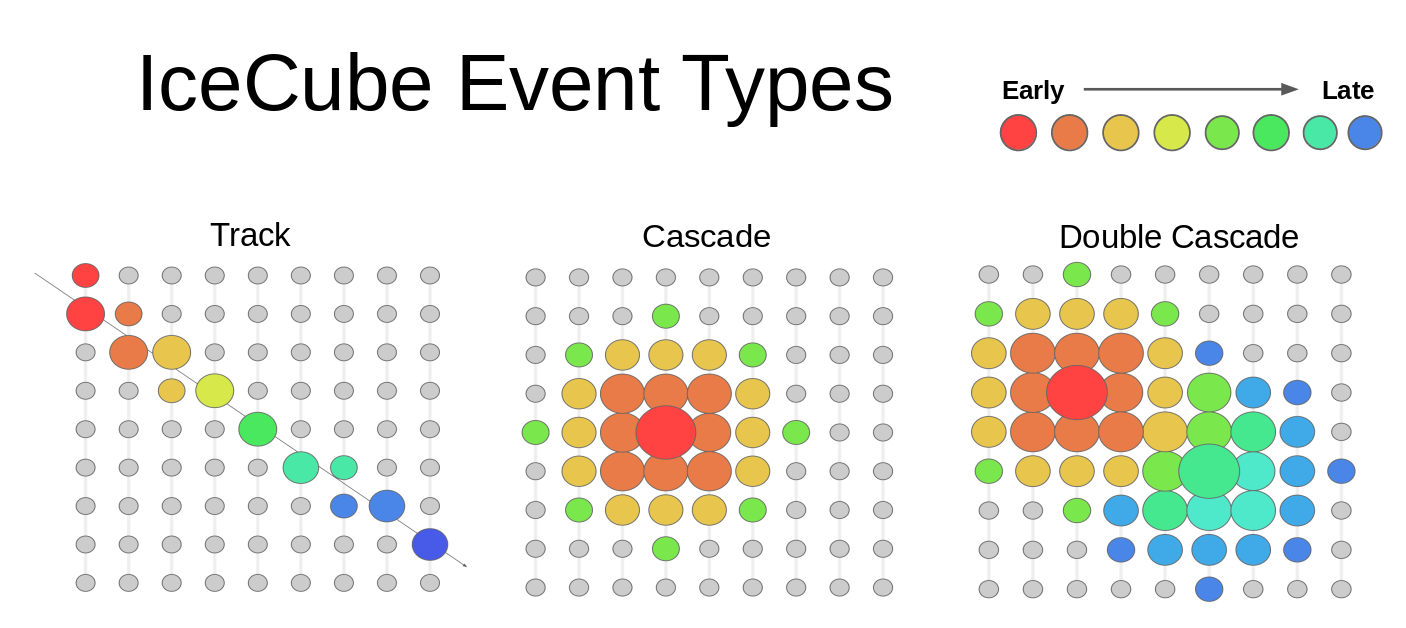
\includegraphics[width=0.8\textwidth]{figs/evt_types.png}
\caption{Cartoons in the x/z plane depicting the various event types seen by the IceCube detector. Grey circles are intended to represent individual DOMs, while colored circles correspond to DOMs that saw photoelectrons. The size of the circle corresponds to the amount of charge seen, while the color denotes the timing. Of most relevance to this work are tracks (left), as their long lever arm provides good pointing resolution.}
\label{fig:evttypes}
\end{figure}


Through-going tracks are notable for their good angular resolution ($<$ 1 degree), particularly at high energies ($> 1$ TeV), as seen in figure \ref{fig:angres}. This makes them an excellent candidate for attempting to do astronomy, as the can be expected to point back to their point of origin with reasonable accuracy. Energy reconstruction of these events is somewhat more challenging, however, due to a combination of stochastic energy losses of the muon producing the cherenkov photons, and the fact that the event itself is often not entirely contained in the detector. The energy resolution of tracks in IceCube is approximately a factor of 2 at 10 TeV, though this increases for higher energy events \cite{10yrpublicdata}.

\begin{figure}[h]
\centering
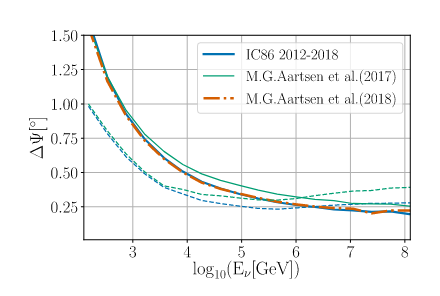
\includegraphics[width=0.8\textwidth]{figs/angres.png}
\caption{The median angle between simulated neutrino and reconstructed muon directions as a function of energy for various high-statistics IceCube samples composed of track events. The dark blue line corresponds to PSTracks v003p02, the light blue line corresponds to PSTracks v002p03, and the orange dashed line corresponds to NorthernTracks v002p06 (see section 1.7 for a description of these data samples). The solid lines describe events in the northern hemisphere, while the dashed lines are events in the southern hemisphere \cite{10yr_tint}\cite{NorthernTracks_PS}\cite{7yr_tint}.}
\label{fig:angres}
\end{figure}

\subsection{Cascades}
In CC interactions, the initial interaction produces a hadronic cascade regardless of the variety of outgoing lepton produced. If the outgoing lepton is an electron, the interaction length is relatively short, typically less than the 125 meter spacing of IceCube strings. Because of this, the resultant pattern of DOM hits in the detector is formed from the combined hadronic and electromagnetic showers. As the two showers occur at approximately the same spatial position, this appears to the detector as a single cascade. While due to their spherical symmetry cascades tend to have poor (10 degree or more) pointing resolution, they have excellent energy resolution, as even for high energy events, the entirety of the cascade is often contained within the detector, making energy reconstruction as simple as counting the total number of cherenkov photons produced. The energy resolution of cascades is approximately 15\%, potentially even lower at higher energies \cite{AustinThesis}.

\subsection{Double Cascades}
If the outgoing lepton from a CC interaction is a tau, then it may travel a relatively short distance before interacting again. If the initial tau is high enough energy, this can produce a signature of two spatially separated hadronic cascades in the detector. If the tau is lower energy, the two cascades may not be spatially resolvable, though may still be able to be identified by examining the waveforms observed by hit DOMs. This type of event was only recently observed in IceCube data \cite{taupaper}. Notably, tau events of these energies are not expected to be produced by atmospheric processes, and consequently this observation provides further evidence of an astrophysical neutrino flux. 

\section{Triggering}
IceCube DOMs are subject to dark noise in the detector originating from PMTs emitting electrons from the cathode in the absence of an external photoelectron. This noise should not be correlated between nearby DOMs, and can be dramatically reduced by imposing the triggering requirement that neighboring DOMs also experience a signal with $\plusminus$ 1 $\mu s$. These hits are classified as "Hard Local Coincidence" (HLC). An eight-channel simple majority trigger (SMT8) is used to trigger a readout window where DOM information is written to file. This trigger requires eight DOMs to have HLC hits within a 5 $\mu$s window. 

Events are further filtered through several additional algorithms to pare down events based on temporal and spatial coincidence of DOM hits. The result is a "Level 2" event rate of approximately 2.5 kHz. These events can be additionally filtered to select specifically for high quality track-like events (originating mostly from atmospheric muons, but also from atmospheric and astrophysical muon neutrinos as well), reducing the event rate to ~Hz. This level of data is often referred to within the collaboration as "Muon Level 3", and primarily consists of through-going track-like events. 

\section{Directional Reconstruction}
In this section we discuss algorithms for reconstructing the direction of through-going track events observed by the IceCube detector. Different algorithms may be used for cascades, though understanding these is unimportant for the remaining content of this thesis. Those who are interested in the reconstruction of cascade and double cascade events can refer to \cite{AustinThesis}.

\subsection{LineFit}
An initial guess for the reconstructed direction of the track can be obtained by ignoring the geometry of the cherenkov cone and the optical properties of the ice, and assuming a plane wave of light traveling along a straight line in the detector. The location of each DOM that observes photons ($\textbf r_i$) can then be written as a line (eq. \ref{linefit1}):

\begin{equation}
    \textbf r_i = \textbf r + \textbf v \cdot t_i
    \label{linefit1}
\end{equation}

Where $t_i$ is the time that the $i$th DOM observes photons, \textbf{r} is the vertex of the track, and \textbf{v} is the velocity of light in the ice. A $\chi^2$ fit can then be preformed to determine the free parameters \textbf{r} and \textbf{v} (eq. \ref{linefit2}):

\begin{equation}
    \chi^2 \equiv \sum_{i=1}^{N_{tot}}(\textbf r_i - \textbf r - \textbf v \cdot t_i)^2
    \label{linefit2}
\end{equation}

This can be solved analytically, resulting in fitted vectors for \textbf{r} and \textbf{v} (eq. \ref{linefit3} and \ref{linefit4}):

\begin{equation}
    \textbf r = \langle \textbf r_i \rangle - \textbf v \cdot \langle t_i \rangle
    \label{linefit3}
\end{equation}

\begin{equation}
    \textbf v = \frac{\langle \textbf r_i \cdot t_i \rangle - \langle \textbf r_i \rangle \cdot \langle t_i \rangle }{\langle t_i^2 \rangle - \langle t_i \rangle^2}
    \label{linefit4}
\end{equation}

This corresponds to a vertex (\textbf{r}) and a direction (\textbf{v}) describing the path of the particle. Further discussion on this topic can be found in \cite{track_reco_paper}.

\subsection{SplineMPE}
An improved reconstruction of the particle direction can be obtained by iterating on the initial LineFit reconstruction described above. The LineFit result is treated as a seed for a likelihood based reconstruction that takes the cherenkov angle and ice properties into account. A description of the specific likelihood components may be found in section 3 of \cite{track_reco_paper}. In the simplest implementation of this likelihood method, only information from the first photoelectron observed by a particular DOM is used. This is referred to as a single photoelectron fit, or "SPEFit". For events that produce multiple hits on a single DOM, this information can be included in the likelihood as well, producing a multi-photoelectron (MPE) fit. Since photons arriving after the first are likely to have experienced at least some scattering, a proper description of the ice properties is necessary for an accurate MPE fit. This is incorporated into the likelihood described in \cite{track_reco_paper} via the use of tabulated timing and light yield distributions for various DOM/photon configurations given an ice model developed from fits to LED flasher data \cite{icemodel_paper}. The information in these tables is stored via a multi-dimensional spline, allowing these tables to be used directly as PDFs in the MPE likelihood, hence the name for this variety of reconstruction: "SplineMPE".

\subsection{Paraboloid}
There is some inherent uncertainty associated with the observation and reconstruction of a particular event. For an event originating from a particular true position, the reconstructed position is expected to be drawn from distribution centered on the true position. Properly describing this distribution is key to characterizing the per-event uncertainty associated with the directional reconstruction, and is important for obtaining accurate results in a point source analysis.

A semi-analytic description of the angular error associated with a particular event can be obtained from the likelihood map associated with the direction reconstruction outlined in the previous section. An ellipse can be fit around the global minimum of the likelihood map, describing a $1 \sigma$ containment region. The ellipse is parameterized by two variables, $\sigma_1$ and $\sigma_2$ describing the scales of the two axes of the ellipse, and an average circularized error can be computed as (eq. \ref{circerr})\cite{paraboloidpaper}:

\begin{equation}
    \sigma_{evt} = \sqrt{\frac{\sigma_1^2 + \sigma_2^2}{2}}
\label{circerr}
\end{equation}

This description can be further improved by comparing this error with the "true error" obtained from examining the difference between the simulated event direction and the corresponding reconstructed direction. By multiplying the above circularized error by the ratio of the reconstructed error to the "true" error, we remove potential bias due to effects not accounted for by the directional reconstruction algorithm. For example, one such effect would be the angle between the incident neutrino and the outgoing muon. Since the reconstruction algorithm only reconstructs the direction of the track associated with the muon, the direction of the neutrino is still technically unknown. While at high energies the muon and it's parent neutrino can be assumed to be colinear, this angle becomes a significant source of uncertainty below 1 TeV. 

\section{Energy Reconstruction}
While the direction of track event in IceCube can be reconstructed with good precision using the methods described previously, reconstructing the energy is more difficult. The primary reason for this is simply a lack of information: since many tracks originate from events neutrino interactions outside of the instrumented volume, the entirety of the muon track is not contained within the detector. This prevents the detector from behaving as a calorimeter, and estimates must be made to extrapolate the initial event energy based on the portion of the track observed. Similar to the directional reconstruction, an energy reconstruction of a particular event can be obtained using a likelihood based approach based on the individual DOM observations. 

At its core, this likelihood approach assumes that the number of detected photoelectrons ($k$) is expected to be poisson distributed with a mean directly proportional to the energy: $\lambda=E \Lambda$ (eq. \ref{erecolh}), where $\Lambda$ is the number of photons the event produces per unit energy:

\begin{equation}
    \mathcal{L} = \frac{(E \Lambda)^k}{k!} e ^ {-E \Lambda}
\label{erecolh}
\end{equation}

Maximizing this likelihood over all $j$ DOMs that see photoelectrons results in the relation (eq. \ref{erecoeq}):

\begin{equation}
    E = \sum{k_j}/\sum{\Lambda_j}
\label{erecoeq}
\end{equation}

Which is largely a statement that the event energy is proportional to the number of observed photons, scaled by some factor that is the sum of the light yield scaling functions $\Lambda_j$. These functions depend on a variety of factors including the geometry and ice optical properties. Much like in the case of the directional reconstruction, these functions are often obtained from tabulated monte carlo data, smoothed with a multi-dimensional spline. 

This likelihood can then be applied to calculate the energy loss rate ($\langle dE/dx \rangle$) of a particular muon. Above 1 TeV, this energy loss rate is roughly proportional to the muon energy. A robust estimate of this rate can be obtained by fitting segmented energy losses along the muon track using the methodology described in \cite{erecopaper}. Once a list of segmented energy losses is calculated, there are several different approaches to converting to a reconstructed energy. 

\begin{itemize}
    \item \textbf{MuEX} takes the average of the segmented energy losses and uses that as an estimate of the energy
    \item \textbf{TruncatedEnergy} first removes the largest 40\% of energy losses before calculating an average, ideally reducing the variance in the calculation of $\langle dE/dx \rangle$. 
\end{itemize}

A comparison of these approaches can be found in \cite{erecopaper}, and both methods provide approximately 35\% precision in $\log_{10}E$ for an initial muon energy of $10^4$ GeV, improving slightly to approximately 30\% in $\log_{10}E$ at higher energies. 

\section{IceCube Event Samples Overview}
As the Icecube detector is capable of doing a wide variety of science, there exists a plethora of event samples used within the collaboration. Even within the context of searches for point sources of astrophysical neutrinos, there exist several event samples of IceCube events, each with their own selection criterion and set of reconstructed parameters. In many cases, the distinguishing features between event selections used in point source analyses are purity and event rate. An ideal point source event sample would have both a high purity of astrophysical events in addition to a high event rate. Unfortunately, this is not possible with the current iteration of the IceCube data, as we observe relatively few events above 100 TeV (where the highest purity of astrophysical events can be achieved), and below 100 TeV there is a significant irreducible background of atmospheric neutrinos. 

For this reason, point source event samples in the IceCube collaboration generally follow two different philosophies. "Low statistics/high purity" samples contain relatively few events, but the events in these samples have a high probability of being astrophysical in origin \cite{Estes} \cite{hese7yr}. By contrast "high statistics/low purity" samples contain a higher number of events, including additional astrophysical events. However in doing so, these samples also include significantly more atmospheric (background) events \cite{stettner2019measurement} \cite{10yr_tint}. In the context of point source searches, these samples typically rely on advanced statistical methods in their analysis pipeline to distinguish between clustered astrophysical signal and isotropic atmospheric background. 

Even within the category of high statistics/low purity samples used for neutrino source searches, there exist multiple samples that are regularly used within the IceCube collaboration. The following sections will briefly outline three such samples that are relevant to the analyses presented later in this work.  

\subsection{PointSourceTracks v002p03}
Starting with Muon level 3 data, this sample applies an additional BDT to attempt to select for well-reconstructed muon neutrino interactions from mis-reconstructed atmospheric muon background. The variables used in this BDT were associated with a track-like event topology, and the BDT was trained using both background data, as well as simulation of both an $E^{-2.0}$ and $E^{-2.7}$ signal. The result is a high-statistics sample of mostly track-like neutrino events in the northern sky, consisting of both atmospheric and astrophysical neutrinos \cite{7yr_tint}. Events in this sample use a SplineMPE reconstruction ("plain" settings, corresponding to a balance of computation time and precision) for the event direction, and a MuEX reconstruction for the event energy.


This sample covers seven years of IceCube data (2008-2015), and was used for the historical untriggered flare analysis of TXS0506+056 \cite{TXS_Archival}, where a $3.5\sigma$ neutrino flare was identified in 2014. 

\subsection{PointSourceTracks v003p02}
Though this sample is oftentimes treated as a "successor" to PointSourceTracks v002p03, it is in many ways a completely new event selection. This sample covers 10 years (2008-2018) of IceCube data. Like v002p03, this sample also starts with Muon level 3 data, however here the BDT is trained to additionally reject cascade-like events in addition to accepting track-like events. Additionally, an improved directional reconstruction is used: the SplineMPE reconstruction algorithm is applied twice, with the second application using the results of the first as a seed, and additionally including the energy estimation. This results in improved angular resolution \cite{TessaThesis}.

This sample additionally requires that events pass some precuts prior the the application of the BDT. Events are only selected if they satisfy the conditions below:

\begin{itemize}
    \item The length of empty track (the portion of the reconstructed track that does not have any associated DOM hits) must be $\leq 400$m
    \item The reconstructed track length must be at least 200m
    \item The number of hit DOMs must be $\geq 12$
    \item The number of DOMs that observe direct (non-scattered) photons must be $\geq 6$
    \item $\cos(\theta_{geo}^2) < 0.2$, where $\theta_{geo}$ is the angle between independent reconstructions calculated for the first and second half of the track only. For a high quality track, both the first half reconstruction and the second half reconstruction should lie almost parallel. 
\end{itemize}

This sample also has different requirements for events observed from the southern sky. The minimum track length and maximum empty track length pre-cuts are applied as in the northern sky, in addition to an additional cut that the initial estimated uncertainty ($\sigma_{paraboloid})$ must be less than 5 degrees. A cut on the likelihood reconstructions is also enforced, requiring $R\log(\mathcal{L}) > 9$, where $R\log(\mathcal{L}$ is the "reduced log likelihood", where the maximum likelihood value, $\mathcal{L}$ is divided by the number of degrees of freedom, $n_{dof}$ ($n_{dof} = 5$ in this particular case). Events in the southern sky are also required to have hits on more than 5 different IceCube strings if the number of direct DOM hits was fewer than 12 \cite{TessaThesis}. 

This sample is notable as it was the sample used for the 10-year all-sky IceCube time integrated analysis, where NGC 1068 was identified as having a significance of $3 \sigma$~\cite{10yr_tint}. This sample has also been publicly released for use outside the IceCube collaboration \cite{10yrpublicdata}.

\subsection{NorthernTracks v002p06}
The NorthernTracks sample is a high statistics, low purity sample of through-going tracks that was originally developed for the purpose of performing a diffuse fit of the atmospheric and astrophysical neutrino spectrum. As such, this sample has relatively good data/MC agreement (as this is essential to the diffuse fit analysis pipeline), but is restricted to only events in the northern sky. Additionally, this sample does not make use of data from DeepCore DOMs,  a decision that was made in order to homogenize the detector. This sample covers 8 years of livetime (2009-2017) has been used for point source analyses as well as diffuse studies of the neutrino spectrum \cite{NorthernTracks_PS}. 

The precuts for this sample in the northern sky are identical to PointSourceTracks v003p02, however this selection then uses two separate BDTs to further filter events: one BDT to select for track-like events, and a separate BDT to reject cascade-like events. In practice the application of these two BDTs is similar, but not perfectly identical, to the application of the single BDT in PointSourceTracks v003p02. Also of note is that the BDTs used in the NorthernTracks selection are trained exclusively using simulation, for both signal and background.

This sample uses a SplineMPE directional reconstruction (with "max" settings, prioritizing precision over computation speed), and a TruncatedEnergy estimator as the energy reconstruction. 

A comparison of the three samples outlined here can be seen in table \ref{tab:evtsamples}

\begin{sidewaystable}
\centering
\begin{tabular*}{0.865\textwidth}{|c|ccc|} 
\hline
. & PSTracks v2 & PSTracks v3 & NorthernTracks\\
\hline\hline
Pre-cuts & No & Yes & Yes\\ 
BDT 1 & Selects tracks & Selects tracks and rejects cascades & Selects tracks \\
BDT 2 & None & None & Rejects cascades \\
Signal training set & Simulation & Simulation & Simulation \\
Background training set & Data & Data & Simulation \\
Direction reconstruction & SplineMPE ("plain") & SplineMPE ("plain")$\times$ 2 & SplineMPE ("max") \\
Angular error estimator & Paraboloid & Paraboloid & Paraboloid \\
Energy estimator & MuEX & MuEX & TruncatedEnergy \\ 
DeepCore included? & Yes & Yes & No \\
Livetime & 7 years (2008-2015) & 10 years (2008-2018) & 8 years (2009-2017) \\
\hline
\end{tabular*}
\label{tab:evtsamples}
\caption{A comparison of several similar high statistics/low purity event samples used by the IceCube collaboration}
\end{sidewaystable}


\chapter{Review and Improvements to Statistical Methods in Neutrino Astronomy}\label{chapter:methods}
Point source searches in neutrino astronomy are essentially weighted clustering analyses: each event is determined by a set of coordinates (right ascension, declination, angular error, and time), and a weight (energy), and the task is to determine if high weight points are clumped beyond what is expected purely from statistical fluctuations. Most attempts to do this make use of a similar approach, using data-driven background estimation and a likelihood-based estimator of clustering. This section outlines the general framework of such an analysis, as well as several variants of the likelihood-based clustering estimator that is commonly used. \color{red}In the simplest case, only spatial clustering is examined, and temporal information is excluded entirely ("time-integrated" analyses), however it can be additionally interesting to explore the possibility of temporal clustering of events as well, increasing the dimensionality of the clustering problem by one. Later in this section we introduce an improved method for fitting ensembles of spatial and temporal clusters of events ("flares") to characterize the data, which is an improvement over existing methods which only make use of information from the most significant flare. This fills in the methodological gap that can be seen in table~\ref{tab:stresults}. \color{black}

\section{Clustering Analysis Outline for an Arbitrary Test Statistic}
There are many ways of constructing a test statistic in neutrino astronomy, in addition to a variety of types of clustering to look for (for example, clustering near various source catalogs, clustering in space and time, clustering with weights according to source/event energy weights, clustering about an extended spatial feature such as the galactic plane). However, almost all clustering analyses in this area share several features in their construction:

\begin{enumerate}
    \item A test statistic is formulated, which ideally tests the degree of clustering of astrophysical events near a particular source candidate location. This test statistic is typically a likelihood-based test statistic of a form similar to that which is described in the following section, however this test statistic is often modified to reflect the specifics of the clustering hypothesis being tested. 
    \item A background test statistic distribution is calculated using maps generated from data that has the right ascension values of events randomized. This destroys any clustering that may have already been present, providing an excellent representation of the null hypothesis (a purely diffuse astrophysical neutrino flux with no spatial or temporal clustering). As this background estimation is data-driven, it is robust against unknown backgrounds that may be present in the sample. Scrambling the data does not affect the sample event content, and consequently the underlying distributions of event declination, energy, and arrival time are unchanged. 
    \item Alternative hypothesis test statistic distributions may be obtained from simulations of signal events. If the analysis is not sensitive to the total astrophysical neutrino flux, simulated events can simply be added to the background maps generated above. If the analysis is sensitive to the total astrophysical flux, then more sophisticated methods (such as moving existing events instead of injecting new events) may be required. Once maps containing signal have been generated, they can be used both to characterize the performance of the analysis, as well as compute upper limits in the event of a null result.
    \item The performance of the test statistic being used is typically evaluated using the \textit{sensitivity} and/or \textit{discovery potential}. The \textit{sensitivity} refers to the amount of signal that needs to be injected before 90\% of the test statistic distribution is greater than the median of the background test statistic distribution. Similarly the \textit{discovery potential} refers to the amount of signal that needs to be injected before 50\% of the test statistic distribution is greater than the $N\sigma$ significance threshold in the background test statistic distribution ($N$ is typically either 3 or 5, but can be other values. This is typically clarified by stating that the value reported is the "N-sigma discovery potential"). "Amount of signal" is intentionally ambiguous here, as different analyses are sensitive to different types of signal. The sensitivity and discovery potential can be cast in terms of any number of variables that may be relevant to a particular analysis. For example, in the time-integrated case, these values are often reported as a flux, however time-dependent analyses may report a fluence, and analyses sensitive to source populations may even report their sensitivity as a curve in the space of source density and source luminosity. 
    \item The test statistic is calculated for the observed data sample, and this observed test statistic is compared to the distribution generated in step 2 to calculate a p-value. This p-value is then used to either accept/reject the null hypothesis of no clustering.
\end{enumerate}

\begin{figure}[h]
\centering
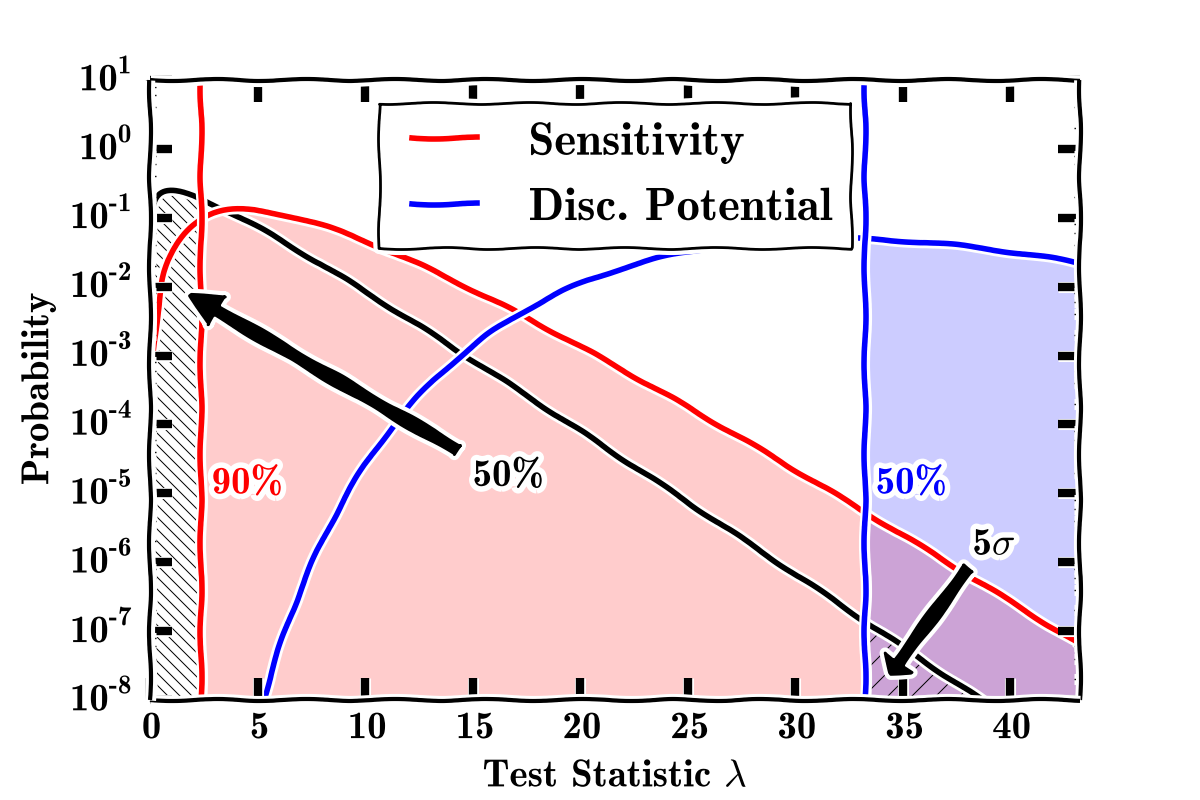
\includegraphics[width=0.8\textwidth]{figs/sens_discpotential.png}
\caption{A toy plot showing the definitions of sensitivity and discovery potential. \cite{Reimann:2019zby}}
\label{fig:angres}
\end{figure}

\section{Unbinned Time Integrated Methods}
Astrophysical point sources may be distinguished from the atmospheric neutrino background by way of clustering: if astrophysical sources are present in the data, events should be clustered near one another, while atmospheric events are expected to be isotropically distributed. Additionally, since high energy neutrino events are more likely to be astrophysical in origin, clustering of these events can be an even stronger indicator of the effect of neutrino point sources in the data. In short, we would like to construct a test statistic that reflects these observations. This can be done by way of a likelihood-based test statistic, using a likelihood composed of signal and background PDFs that describe the spatial and energy properties of events relative to a source candidate location. For a neutrino sample composed of $N$ total events, the likelihood of the data for some number of signal (clustered astrophysical) events, $n_s$ is (eq. \ref{psllh})\cite{Braun_2010}:

\begin{equation}
    \mathcal{L}(n_s, \gamma) = \prod_{i=1}^{N}[\frac{n_s}{N}S_i+(1-\frac{n_s}{N})B_i]
    \label{psllh}
\end{equation}

Where here, $S_i$ and $B_i$ are PDFs that describe the spatial and energy distributions of signal and background events relative to the source candidate location. $S_i$ and $B_i$ are themselves composed of spatial and energy components (eq. \ref{spaceEcomponents_sig} and \ref{spaceEcomponents_bg}). 

\begin{equation}
    S_i = R(r_i) \times \mathcal{E}(E_i, \delta_i|\gamma)
    \label{spaceEcomponents_sig}
\end{equation}
\begin{equation}
    B_i = \frac{1}{\Omega}\times \mathcal{E}(E_i,\delta_i|Atm_{\nu})
    \label{spaceEcomponents_bg}
\end{equation}

Note that the source spectral index, $\gamma$, enters as a free parameter in the energy portion of the signal PDF. 

For the background PDF, the construction is relatively straightforward: background events originate from all directions equally, so the only effect that produces anisotropies is the detector acceptance. Since the IceCube detector acceptance does not vary as a function of right ascension, we can define $B_i$ for a particular declination band to simply be $1/\Omega$, where $\Omega$ is the solid angle of a declination band centered on the source candidate declination. Similarly, the background energy PDF can be obtained by measuring the energy distribution of observed events as a function of declination. 2D histograms of event counts as a function of declination and event energy are assembled, and these distributions are then splined to create PDFs that can be used to evaluate $B_i$ for events at an arbitrary declination and energy. 

\begin{figure}[h]
\centering
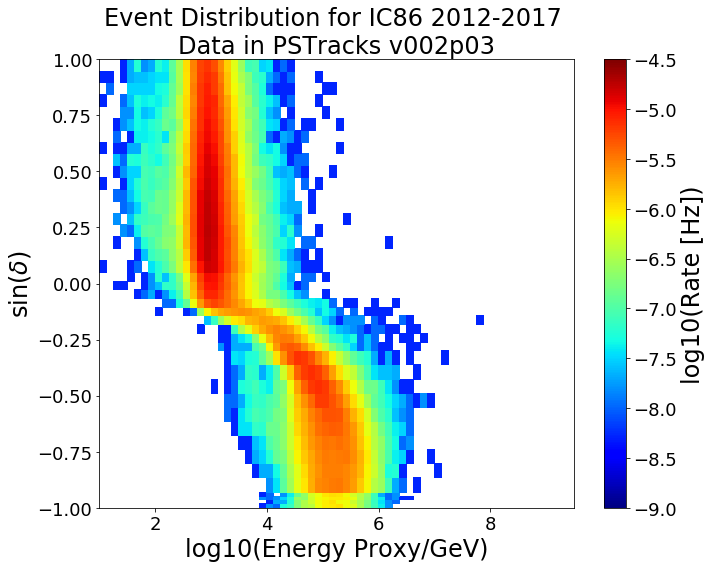
\includegraphics[width=0.4\textwidth]{figs/psv2_edec.png}
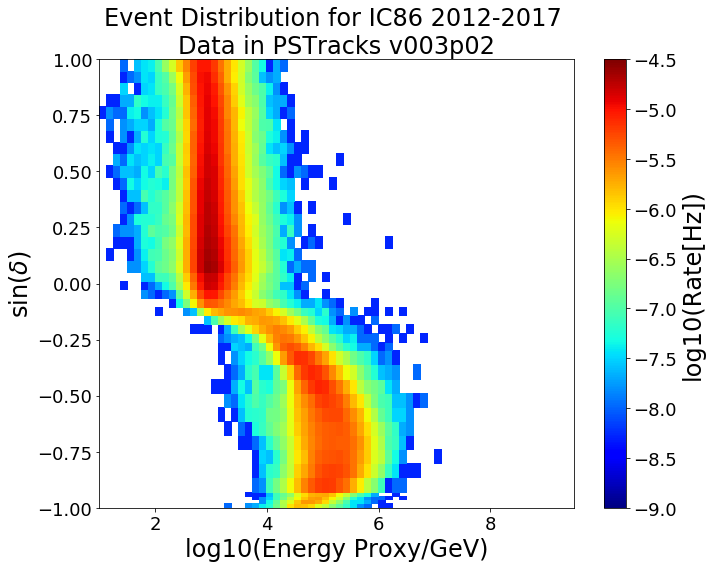
\includegraphics[width=0.4\textwidth]{figs/psv3_edec.png}
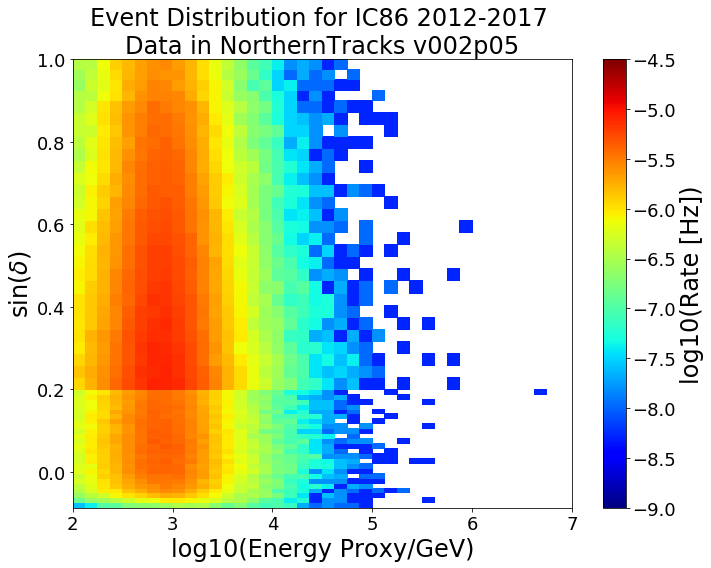
\includegraphics[width=0.4\textwidth]{figs/nt_edec.png}
\caption{2D histograms of declination and energy proxy for the 3 IceCube track event samples discussed in this document: PointSourceTracks v002p03 (left), PointSourceTracks v003p02 (right) and NorthernTracks v005p02 (bottom). Splines of these distributions are used as background PDFs in the clustering likelihood described in equation~\ref{psllh}\cite{10yrpublicdata}. The NorthernTracks dataset is restricted to the northern sky, and additionally the splines associated with this dataset use finer binning near the horizon, hence the seeming dicontinuity near $\sin(\delta)=0.2$}
\label{fig:DecEnDist}
\end{figure}

Unlike background events, signal events are expected to be clustered near the source candidate location. For this reason, the spatial component of the signal PDF, $R(r_i)$, is assumed to be a 2-D gaussian centered on the source candidate location (eq. \ref{sigspacepdf}):

\begin{equation}
    R(r_i) = \frac{1}{2\pi\sigma_{i}^2} e ^{-\frac{r_i^2}{2\sigma_i^2}}
    \label{sigspacepdf}
\end{equation}

Where $r_i$ is the angular distance between the $i$th event and the source candidate location and $\sigma_i$ is the event angular error.  

The energy component of $S_i$ is obtained from simulation: Simulated events are weighted according to a particular astrophysical spectral index, creating a 2D PDF describing the sum of simulated event weights as a function of declination and energy. These maps are then divided by the background PDF described above to create a map describing the "signalness" of events at a particular energy and declination, given a spectral index. As these maps are created for a range of spectral index values (typically ranging between $\gamma=1$ and $\gamma=4$), a 3-D PDF of event energy, declination, and spectral index hypothesis results from this process. This is precisely the function $\mathcal{E}(E_i, \delta_i|\gamma)$ that enters the likelihood, and can be used to fit for $\gamma$, given events observed at declination $\delta$ with energy $E_i$.  

\begin{figure}[h]
\centering
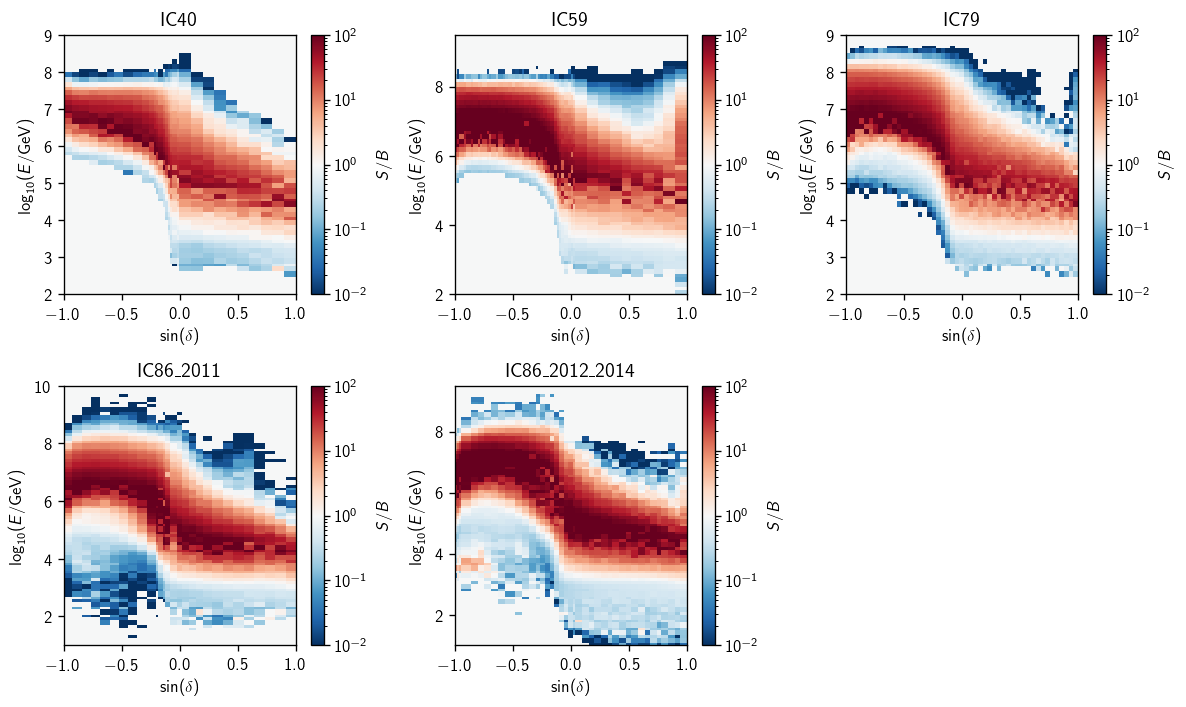
\includegraphics[width=0.8\textwidth]{figs/sig_hists.png}
\caption{Signal PDFs associated with a $\gamma=2.0$ spectral index hypothesis, assembled from PSTracks v002p03. Similar PDFs are constructed for spectral indices ranging from $\gamma=1.0$ to $\gamma=4.0$, thereby constructing a 3-D PDF that can be used in the point source likelihood.}
\label{fig:SigPDf}
\end{figure}

The likelihood described in eq. \ref{psllh} can be maximized as a function of $\n_s$ and $\gamma$, resulting in best fit parameters $\hat{n_s}$ and $\hat{gamma}$. We can then compute a test statistic for a given data sample from the likelihood ratio (\ref{psts}):

\begin{equation}
    TS = -2 \log \frac{\mathcal{L}(n_s=0)}{\mathcal{L}(\hat{n}_s, \hat{\gamma})}
    \label{psts}
\end{equation}

This test statistic can then be used in the generalized framework described in the sections above to test the hypothesis of spatial clustering of astrophysical neutrino events near a particular source location. 

This framework can be applied to multiple locations at once, and the results combined by summing the individual test statistics calculated at each location (note that this is equivalent to calculating the product of the likelihoods). This process is often referred to as "source stacking", and can be used to improve sensitivity to dim sources, provided there are multiple emitters in the source candidate list. 

Other methods of combining information across multiple source locations exist as well. In particular, the binomial test is a popular way of doing this. Give a list of source candidates and their associated p-values, we can search for the most significant combination of source candidates by employing the binomial test-statistic (eq. \ref{bitest})

\begin{equation}
    p(k) = \sum_{i=k}^{N_{eff}} \binom{N_{eff}}{i}p_k^i(1-p_k)^{N_{eff}-i}
    \label{bitest}
\end{equation}

Where $p(k)$ is the p-value associated with combining the results of the $k$ most significant sources, $N_{eff}$ is the effective number of trials (often simply equal to the total number of source candidates), and $p_k$ is the p-value of the $k$th most significant source. The minimum of p(k) can then be computed and treated as a test statistic, to obtain a p-value associated with the best-fit number of sources ($k_{min}$) in a particular catalog. 


\section{Unbinned Time-Dependent Methods}
In addition to being clustered in space, astrophysical neutrino events may also be clustered in time (a neutrino "flare"). Accounting for this temporal clustering may allow us to identify sources that are insignificant under a corresponding time integrated analysis. Studying the temporal variation of source candidates can also inform us of the specifics of the source dynamics of particle production, as the time scale of observed flares is related to the physical scale of the astrophysical objects in which particle production is occurring. This method was used in ~\cite{txs_archival} to identify the 2014 neutrino flare candidate with a significance of $3.5 \sigma$. 

\subsection{Optimizing for a Single Flare}
We can modify our time-integrated likelihood to account for potential temporal clustering as well by simply appending a temporal PDF to the existing PDFs that describe the spatial and energy components of the analysis (eq. \ref{tmodllh1}, \ref{tmodllh2}):

\begin{equation}
    S_i = R(r_i) \times \mathcal{E}(E_i, \delta_i|\gamma) \times \mathcal{T}(t_i)
    \label{tmodllh1}
\end{equation}

\begin{equation}
    B_i = \frac{1}{\Omega}\times \mathcal{E}(E_i,\delta_i|Atm_{\nu}) \times \frac{1}{\delta T}
    \label{tmodllh2}
\end{equation}

Where $\delta T$ is the full livetime of the sample, and the associated temporal background PDF is $1/\delta T$, as the background event rate should be constant. In practice, this is assembled in a data-driven manner by measuring the data sample event rate in each of the 8-hour segments ("runs") that are used to segment the data. In this way, seasonal variations of the detector event rate are accounted for by the likelihood, as the flare candidates are always being compared to the local event rate in time.

\begin{figure}[h]
\centering
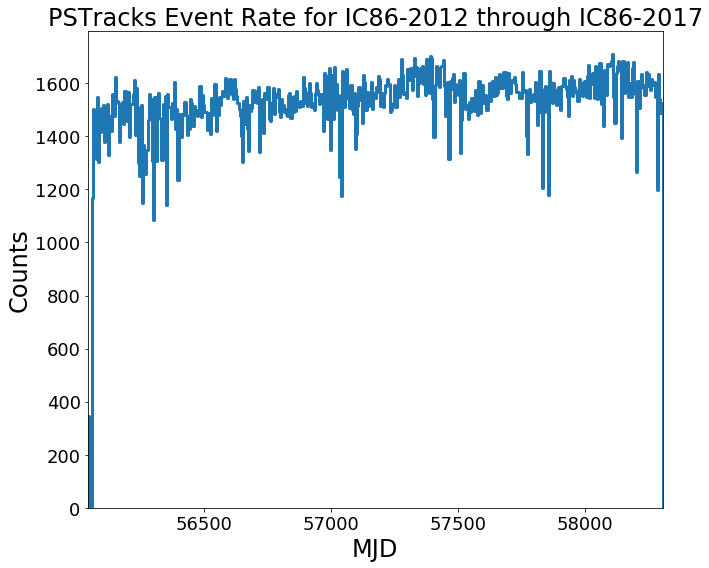
\includegraphics[width=0.8\textwidth]{figs/evt_rate.png}
\caption{The event rate of the IC86 seasons of the PointSourceTracks v3 data sample. This event rate can be used to generate a background temporal PDF in the time-dependent clustering likelihood.}
\label{fig:evt_rate}
\end{figure}

The temporal contribution to the signal PDF, $\mathcal{T}(t_i)$, can take various forms depending on the particular shape that one assumes for the time profile of flare candidates, but the most basic temporal profile can be used is a box (eq. \ref{boxflare}):

\begin{equation}
    \mathcal{T}(t_i | t_0, \Delta t) = 
    \begin{cases} 
      0 & t_i < t_0 \\
      \frac{1}{\Delta t} & t_0 \leq t_i \leq t_0+\Delta t \\
      0 & t_i > t_0 + \Delta t
   \end{cases}
   \label{boxflare}
\end{equation}

This box-shaped temporal PDF essentially asks as a mask, filtering for events that occur within the time window between $t_0$ and $t_0 + \Delta t$. The events within this time window then contribute to the likelihood in a similar manner to the time-integrated case. Note that by adding this temporal PDF to the likelihood, we have also introduced 2 new parameters that the likelihood can be maximized with respect to: $t_0$ and $\Delta T$, which describe the flare start time and duration, respectively. 

Similar to the time-integrated case, a likelihood ratio test statistic can be assembled from this likelihood, however this test statistic can be further improved in the time-dependent case by accounting for the duration of flare candidates that were scanned over (eq. \ref{psts_tdep}:

\begin{equation}
    TS = -2 \log [\frac{\Delta T}{\hat{\Delta t}}\frac{\mathcal{L}(n_s=0)}{\mathcal{L}(\hat{n}_s, \hat{\gamma}, \hat{t}_0, \hat{\Delta t}}]
    \label{psts_tdep}
\end{equation}

Where the the factor $\frac{\Delta T}{\Delta t}$ can be interpreted as a trial factor that accounts for the fact that there are significantly more short flare candidates that can be tested than long ones (e.g. there is only 1 potential flare candidate with $\Delta t = \Delta T$, but there are many flares that can be made with $\Delta t = \Delta T/100$). This factor normalizes the test statistic scale between short and long flares \cite{Braun_2010}.

In practice, this process is extremely computationally intensive due to the number of likelihood minimizations that need to be performed. This can be mitigated by seeding flares with events that already have a high probability of being signal in origin, based off their energy and arrival direction. An ensemble of seed events can be defined to the set of events with $S_i/B_i$ greater than some threshold value, where $S_i$ and $B_i$ refer to the signal and background PDF components of the time integrated likelihood (describing only the spatial and energy properties of contributing events). Typically this threshold is set to be relatively low ($S_i/B_i > 1$), however higher values can also be used if computational requirements are particularly stringent (e.g. if running over the entire sky). 

Many analyses compute the test statistic in eq. \ref{psts_tdep} for a variety of flare candidates, and then use the flare with the maximum test statistic as the "best-fit" flare. The test statistic associated with this "best-fit" flare is then compared to a distribution of "best-fit" flares obtained from the background case (generated from data scrambled in right ascension), resulting in a p-value that describes the strength of the clustering hypothesis relative the the null hypothesis of no clustering. 

In simulated signal trials, the likelihood-based flare test statistic is able to reconstruct the injected number of signal events in each flare with reasonable accuracy, and the per-flare spectral index fits show similar agreement as well. 

\begin{figure}[h]
\centering
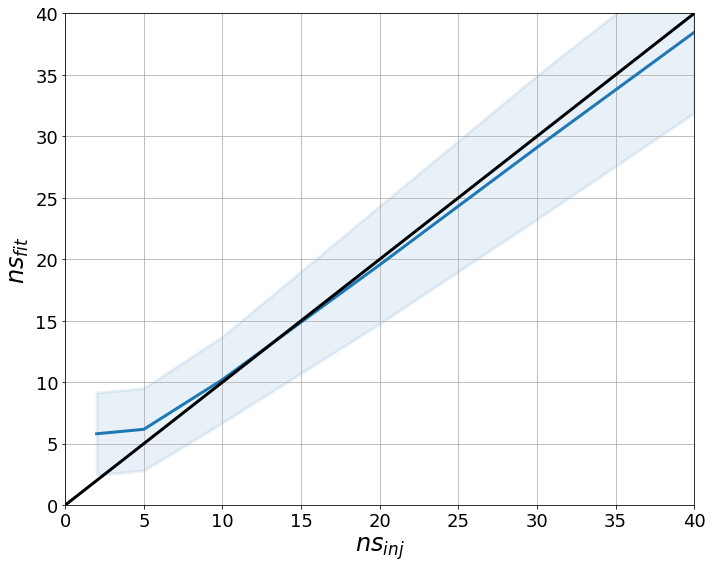
\includegraphics[width=0.4\textwidth]{figs/nsfit.png}
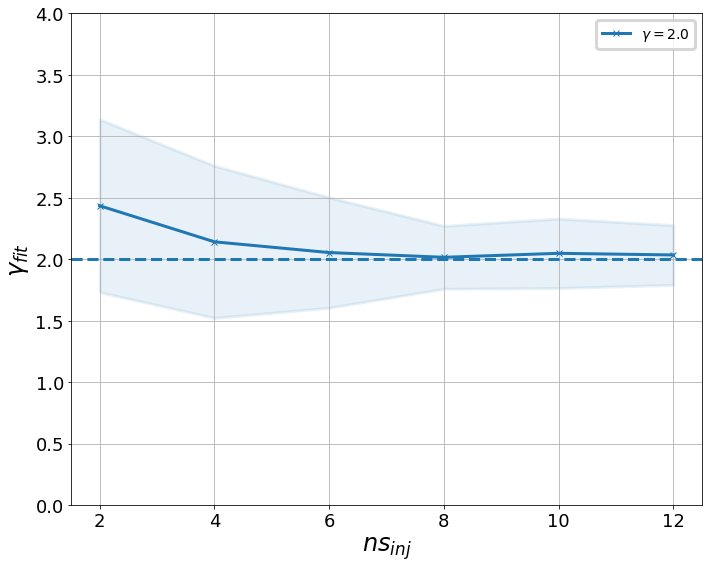
\includegraphics[width=0.4\textwidth]{figs/gamfit_2.0.png}
\caption{The best fit number of signal events in a flare, and the best fit spectral index versus the true number of signal events injected in simulated trials. On average, for flares with $> \approx 5$ events, the time-dependent likelihood is able to accurate estimate the true number of signal events.}
\label{fig:perflare_nsfit}
\end{figure}


\subsection{Improving the Search for Temporal Clustering: Fitting Ensembles of Multiple Flares}
As the IceCube detector collects more data, it becomes increasingly useful to be able to test the hypothesis of multiple neutrino flares that may have occurred at a particular location. Fitting only the largest flare is advantageous if the source flare rate is expected to be low enough that sources only flare once over the data-taking period, however if sources flare multiple times the single-flare analysis potentially misses a significant amount of useful information. \color{red}By incorporating information from multiple flares at a particular location, an analysis can be sensitive to a smaller individual flare intensity. This is analagous to spatial stacking analyses, as can be seen in table~\ref{tab:stresults}, but we have additionally improved our algorithm to stack \textit{flares} instead of just spatial source candidates. In this section we discuss the construction of this method, and the following sections describe the results of the first applications of this method to various source catalogs. \color{black}

The process of fitting multiple flares at a particular source candidate location is similar to the single-flare maximization procedure described above. Flare candidates are seeded by events with a high $S_i/B_i$ ratio near the candidate location. For each flare candidate, the test statistic described in equation \ref{psts_tdep} is calculated. Unlike the single flare case, these flare candidates are then ordered by decreasing test statistic value, and any flares that overlap in time with a different flare that itself has a higher test statistic are removed. Additionally, any flares with a test statistic $< 0$ are removed. What remains is a temporally decorrelated ensemble of flare candidates, each with $TS>0.$. This ensemble functions as a neutrino "flare curve" (similar to light curves produced by photon-based telescopes), that describes the temporal variability of the signal originating from a source candidate location. A "multi-flare" test statistic describing the significance of the temporal variability of this source candidate can then be calculated as the sum of the individual flare candidate test statistics (eq. \ref{multiflareTS}):

\begin{equation}
    \widetilde{TS} = \sum_{j=0}^{N_{flares}} TS_{j}
    \label{multiflareTS}
\end{equation}

Where here, $j$ is an index that refers to the individual flares that compose the neutrino flare curve. This test statistic can then be compared to an ensemble of similar test statistics generated from right-ascension scrambled (background) data to obtain a final p-value describing the significance of the set of flares that were fit at a particular source candidate location. 

An estimation of the total number of signal events can be obtained in a similar manner (eq. \ref{mfns}), where the total number of signal events associated with a particular source candidate is just the sum of the best-fit number of $n_s$ in each contributing flare candidate:

\begin{equation}
    \widetilde{n}_s = \sum_{j=0}^{N_{flares}} \hat{n}_{sj}
    \label{mfns}
\end{equation}

Note that this similar to time-integrated source stacking mentioned above, however instead of stacking test statistics associated with spatially distinct locations, we are instead stacking spatially and temporally distinct \textit{flares}.

The multi-flare algorithm is, in some sense, inclusive of the single flare algorithm: by fitting all the flares at a source candidate location, we have obviously also fit for the largest flare. It is thus trivial to obtain the single-flare significance once the multi-flare result is obtained. In order to do this, simply compare the highest flare candidate test statistic that was obtained with a distribution of single-flare test statistics obtained in a similar manner from background (right-ascension scrambled) data. 

In addition to calculating the local significance of the largest flare, the local significance of the other flare candidates composing the flare curve fit by the multi-flare algorithm can also be obtained in a similar manner. We can define the "local significance" of a particular flare (not necessarily the largest) to be the fraction of flares in the background distribution with $TS_j>TS_{j,observed}$. Note however, that the calculation of multi-flare significance is done in the space of $TS_j$, not the space of the corresponding local significances $p_j$. This means that the multi-flare significance is \textit{not} simply the product of the component flare $p_j$'s, as each flare is not entirely statistically independent from the others (e.g. once the largest flare is fit, the remaining available livetime in which other flares can be fit is reduced by an amount equal to the duration of the largest flare.) 

\begin{figure}[h]
\centering
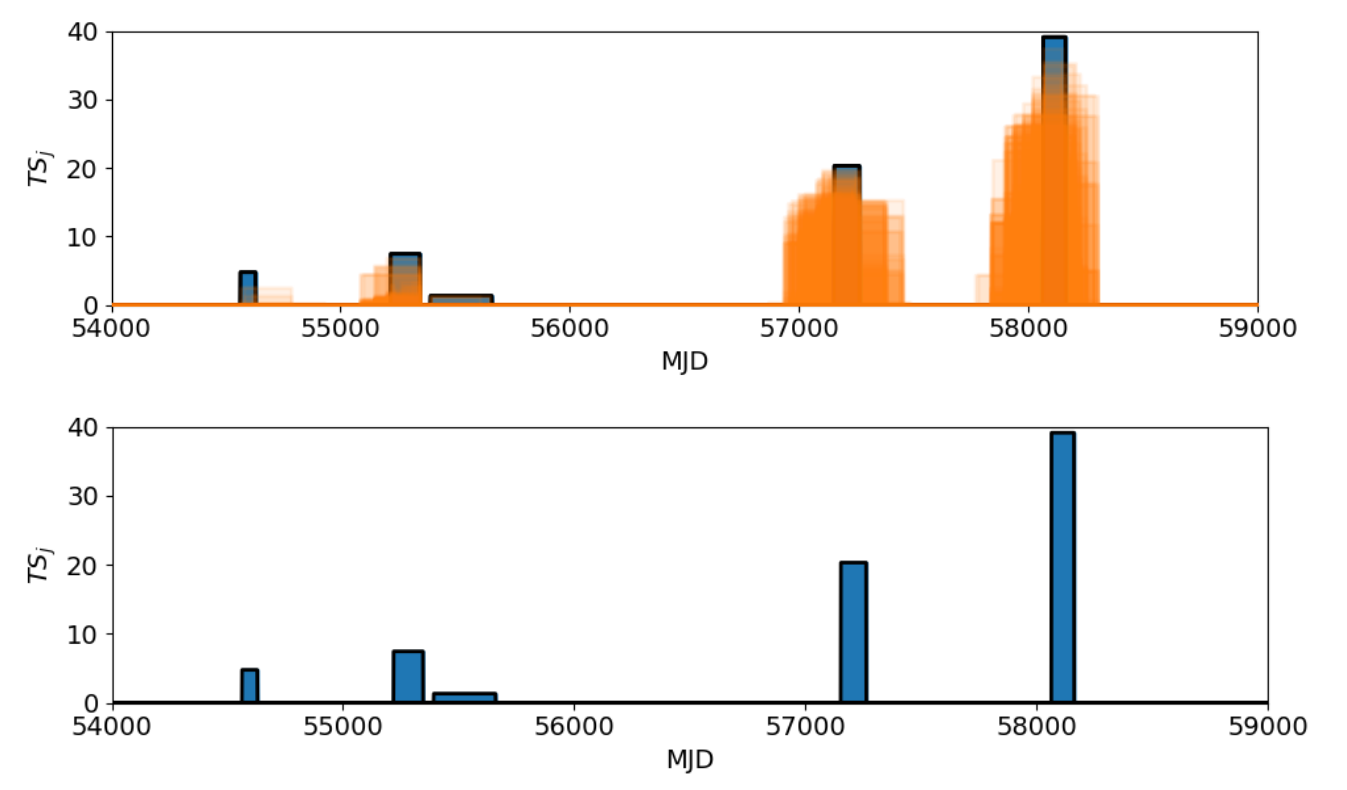
\includegraphics[width=0.8\textwidth]{figs/mf_algorithm.png}
\caption{A graphical example of the progression of the multi-flare decorrelation algorithm. Colored boxes represent flare candidates that were tested, seeded by events with high $S_i/B_i$ ratios. The height of each box corresponds to the individual flare candidate test statistic, $TS_j$. Orange flares overlap with another flare with a higher test statistic, and are consequently removed, leaving only the blue flares. The test statistics of the blue flares are then summed, and can be used for hypothesis testing of flaring neutrino emission at this source candidate location.}
\label{fig:mf_algorithm}
\end{figure}


As mentioned above, the multi-flare algorithms is particularly useful in the case of several similarly sized flares. In this case, while the single flare algorithms will identify the correct number of events in the largest flare, the estimation of the total number of signal events associated with the source candidate will be incorrect (as there is a non-negligible portion of events that belong to flares that were not identified by the single flare algorithm). By contrast, the multiflare algorithm improves the estimation of $n_s$ in the case of multiple similarly sized flares, as signal events in all flare candidates (not just the largest one) are able to contribute. This improvement is shown in figure \ref{fig:persrc_nsfit}.

\begin{figure}[h]
\centering
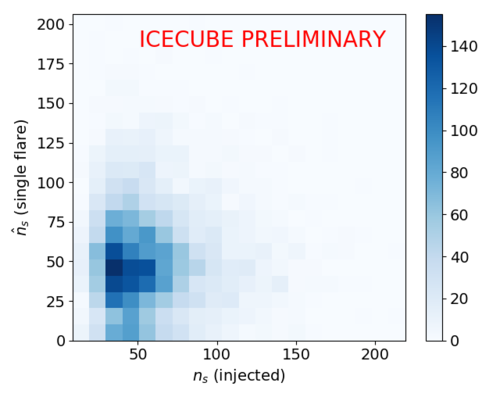
\includegraphics[width=0.4\textwidth]{figs/500px-Ns_singleflare.png}
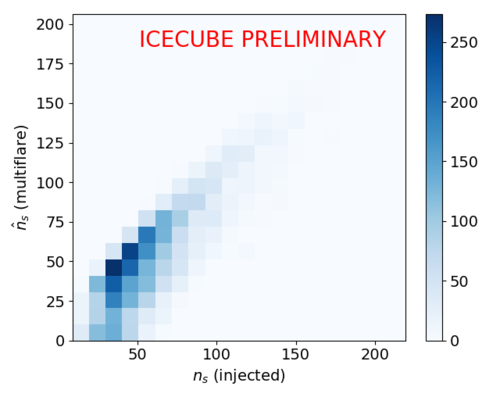
\includegraphics[width=0.4\textwidth]{figs/500px-Ns_multiflare.png}
\caption{Left: the injected vs. fit number of signal events when attempting to use the single flare algorithm to describe an ensemble of neutrino flares. Right: The same plot, but using the multiflare estimation of $n_s$ that accounts for signal events in all flare candidates.}
\label{fig:persrc_nsfit}
\end{figure}

As an example of a case where the multi-flare algorithm is advantageous, consider the case shown in \ref{fig:mf_example}, which has 3 flares injected at MJD=55246.3, 55807.4, and 57632.7 at a test location of (RA, Dec) = ($77.45^{\circ}$, $5.61^{\circ}$). The single flare method fits only the flare at MJD = 55246.3 (with TS = 22.66), while the multiflare method fits all flares together, with a multi-flare test statistic of $\widetilde{TS}$ = 60.52. While the largest individual flare only has a significance of $3.29 \sigma$, by combining information from all the flares that were fit at this location, we arrive at a multi-flare significance of $4.7 \sigma$. 

\begin{figure}[h]
\centering
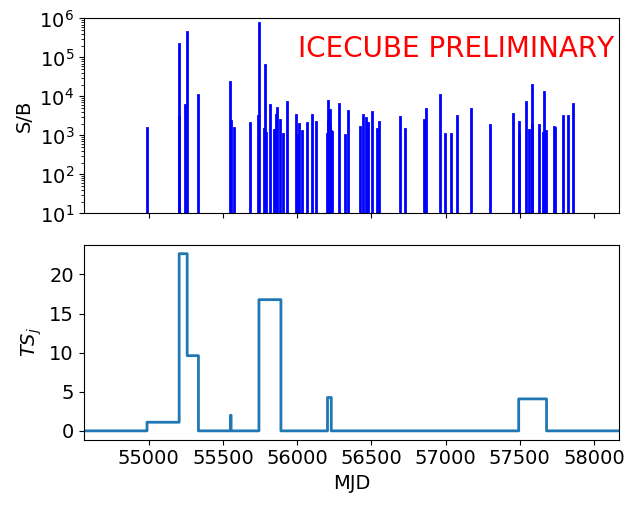
\includegraphics[width=0.45\textwidth]{figs/example_flarecurve.png}
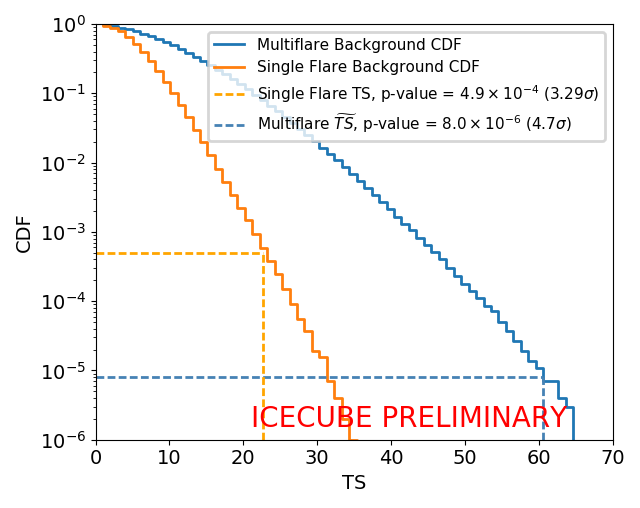
\includegraphics[width=0.45\textwidth]{figs/1src_1k_bgdist.png}
\caption{Left, top: Events that pass the $S/B$ threshold cut for generating windows, for a source located at (ra, dec) = ($77.45^{\circ}$, $5.61^{\circ}$). There are 3 injected flares, centered at MJD=55246.3, 55807.4, and 57632.7. Left, bottom: The single flare method fits only the flare at MJD = 55246.3 (with TS = 22.66), while the multiflare method fits all flares together, with a global test statistic of $\widetilde{TS}$ = 60.52. Right: The background test statistic distributions for a single source, located at declination = $5.61^{\circ}$. The background multiflare test statistic distribution is shown in blue, while the single flare method is shown in orange. The vertical lines represent the test statistics associated with the flare curve on the left The single flare p-value for this source is $4.9 \times 10^{-4}$ (3.29$\sigma$), while the multiflare p-value is $8.0 \times 10^{-6}$ ($4.7\sigma$). }
\label{fig:mf_example}
\end{figure}



\chapter{Applications of the Multi-flare Algorithm to Source Catalogs}\label{chapter:catalogsearches}
The multi-flare algorithm introduced in the previous section may be applied to an ensemble of sources that share common features. This is common practice in neutrino astronomy, as examining emission from a catalog allows us to explore the possibility of neutrino emission from a class of sources, rather than a specific individual source. 
Here, we explore two catalogs designed to explore source features related to those associated with the analysis of TXS 0506+056. Namely, the fact that the analysis was initially triggered by a high-energy neutrino event, and also the fact that TXS 0506+056 is a blazar. For the former, we assemble a catalog of high energy IceCube events to treat as ``sources" (a ``self-triggered" catalog analysis), while for the latter we use the pre-existing catalog of Fermi 3LAC blazars~\cite{fermi_3lac}.

In both cases, the multi-flare algorithm is applied at each source candidate location, resulting in a multi-flare test statistic (and corresponding pre-trial p-value) associated with each source candidate.
To test for potential sub-populations of strong emitters within the catalog, we additionally calculate a best-fit number of multi-flare sources via iteratively summing the sources with the largest test statistics (\ref{iterativesum}). For a given data set, the sources are ordered by their multiflare test statistic, $\widetilde{TS}$. A p-value for $k=1,2,3,...N_{srcs}$ is calculated, and subsequently the $k$ that produces the minimum p-value is selected ($k_{best}$).

\begin{equation}
    \widetilde{TS}_{all} = \sum_{m=0}^{k_{best}}\widetilde{TS}_m
\label{iterativesum}
\end{equation}

An additional trial factor is then calculated by applying this procedure to maps of data with randomized right ascension values to assemble a distribution of $\widetilde{TS}_{all}$ representative of the null hypothesis. A final p-value can then be obtained by comparing an observed $\widetilde{TS}_{all}$ with this null hypothesis distribution. 

For all the analyses detailed in this section, the NorthernTracksv002p05 sample was used. This sample is described earlier in this document (section 2.5). 

\section{Self-Triggered Catalog}
For this catalog, we select the locations of all the events in the NorthernTracks v002p05 data sample that have a reconstructed energy proxy greater than 200 TeV. This energy threshold is chosen as it is roughly the point where 50\% or more of neutrino events are expected to be astrophysical in origin. We can consequently expect that this catalog contains a non-negligible number of astrophysical neutrino sources, and can test the hypothesis of additional time dependent neutrino emission from these locations. Events that have been selected as source candidates for the catalog are subsequently removed from the sample, and do not otherwise contribute to the calculation of a multi-flare test statistic. 

This catalog contains 32 source candidates, all in the northern sky, and can be seen in figure~\ref{stcat}. Notably, this catalog does not include IC170922A (the alert event that triggered the followup analysis on TXS 0506+056), as at the time this analysis was conducted, the data sample does not extend past the 2015 season, and IC170922A occurred in the 2017 season. 

\begin{figure}[h]
\centering
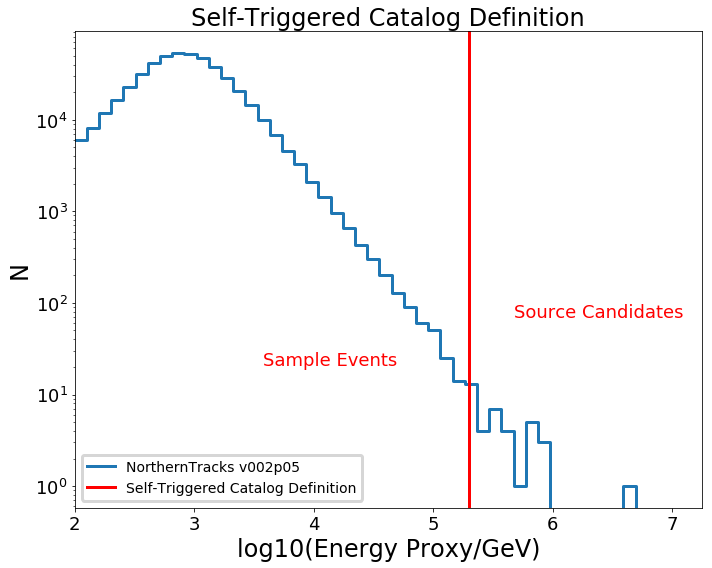
\includegraphics[width=0.4\textwidth]{figs/stcat_def.png}
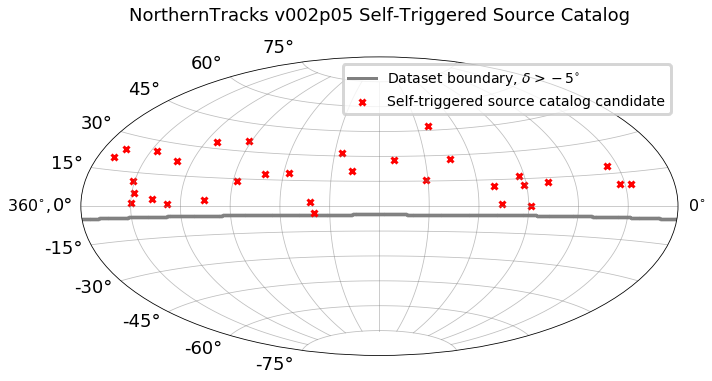
\includegraphics[width=0.4\textwidth]{figs/Selftriggeredcat.png}
\caption{Left: The self-triggered catalog definition: Events with energy proxies to the right of the vertical red line (200 TeV) are treated as source candidates. Events to the left of the red line are then investigated for clustering around the locations of the source candidate events. Right: The self-triggered catalog assembled from the NorthernTracks v002p05 data sample, consisting of all events in the sample with reconstructed energy proxy greater than 200 TeV. The locations of these events are treated as source candidates for the purposes of applying the multi-flare algorithm, however the events themselves are removed from the sample prior to calculating a test statistic.}
\label{fig:stcat}
\end{figure}

Applying the multi-flare algorithm described above to this catalog of the locations of 32 high energy neutrino events results in a best-fit number of sources of $k_{best}=4$, with an associated p-value of $p=0.017$ ($2.13\sigma)$, shown in figure~\ref{fig:stresults}. Detailed results for all 32 source candidates, including fitted number of events and pre-trial p-values, can be viewed in table~\ref{tab:stresults}. 

As mentioned in previous sections, a significant advantage of the multi-flare algorithm is the generation of neutrino ``light curves" (or ``flare curves") that show the historical activity of a source candidate. The flare curves associated with the 4 most significant sources in the self-triggered catalog can be seen in figure~\ref{fig:stcurves}.

\begin{figure}[h]
\centering
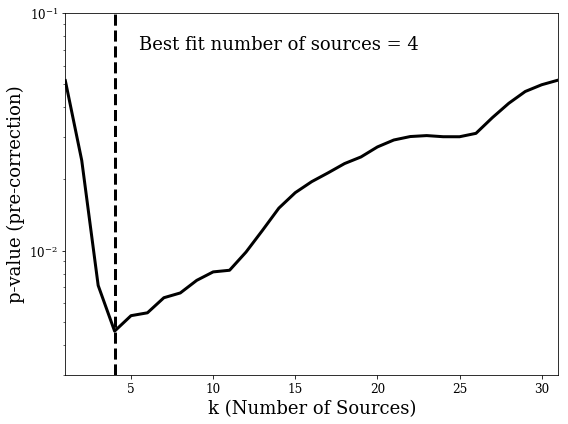
\includegraphics[width=0.4\textwidth]{figs/st_pcurve.png}
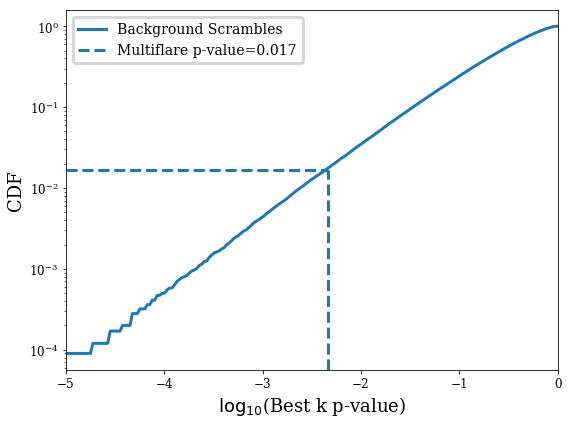
\includegraphics[width=0.4\textwidth]{figs/st_obsresult.png}
\caption{Left: The local significance of stacking the $k$ highest test statistic sources, as a function of $k$. The best fit value of $k=4$ can be seen as the minimum of this curve. Right: The trial corrected result for stacking the top 4 sources together, shown as a vertical line superimposed on the background distribution obtained by applying the algorithm to right-ascension scrambled data.}
\label{fig:stresults}
\end{figure}

\begin{table}[h!]
\centering
 \begin{tabular}{||c c c c||} 
 \hline
 RA & Dec & $\hat{n}_s$ & $p$ (pre-trial) \\ [0.5ex] 
 \hline\hline
 36.69 & 18.32 & 47.21 & 0.00197 \\ 
 \hline
 272.14 & 35.66 & 30.71 & 0.00729 \\
 \hline
 170.19 & 27.85 & 45.75 & 0.00834 \\
 \hline
 93.26 & 16.33 & 30.02 & 0.02667 \\
 \hline
\end{tabular}
\caption{The top 4 most significant multi-flare source candidates in the self-triggered catalog composed of high energy IceCube neutrino events. Collectively, these sources form an excess with a significance of $p=0.017$.}
\label{tab:stresults}
\end{table}


\begin{figure}[h]
\centering
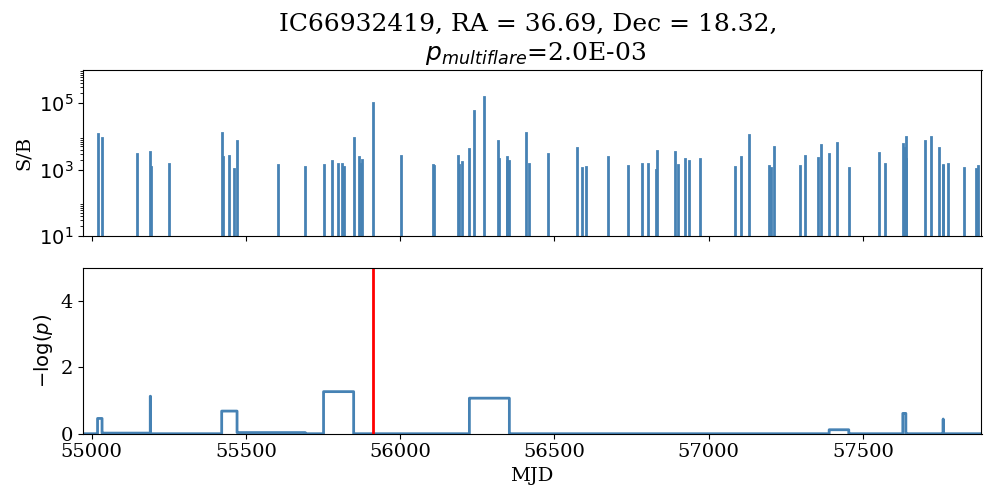
\includegraphics[width=0.4\textwidth]{figs/66932419.png}
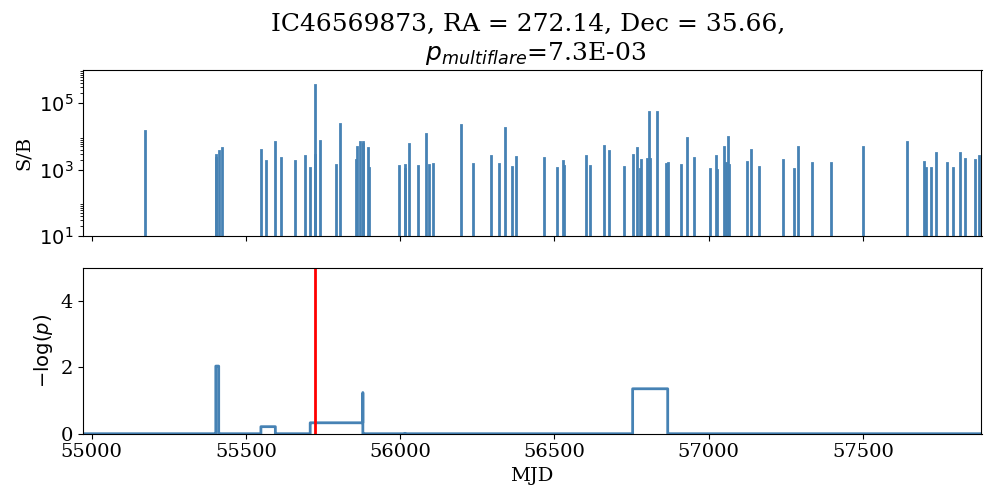
\includegraphics[width=0.4\textwidth]{figs/46569873.png}
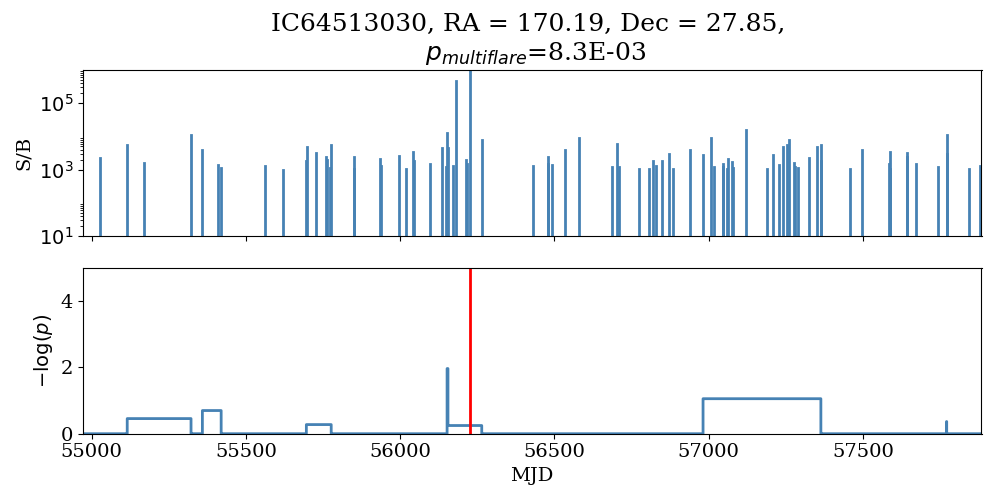
\includegraphics[width=0.4\textwidth]{figs/64513030.png}
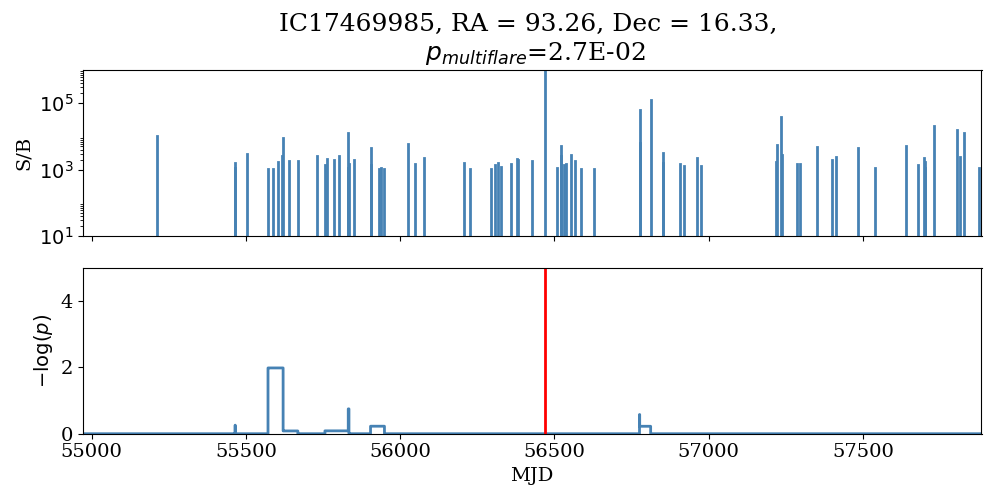
\includegraphics[width=0.4\textwidth]{figs/17469985.png}
\caption{The neutrino ``flare curves" associated with the 4 most significant multiflare source candidates in the self-triggered catalog. The top panel of each subplot shows the event weights, calculated by taking the ratio of the spatial and energy components of the signal and background PDFs described in equation~\ref{spaceEcomponents_sig} and \ref{spaceEcomponents_bg}, while the bottom panels show the fitted ensemble of decorrelated flares, with the local per-flare p-value plotted on the y-axis. The vertical red line denotes the arrival time of the high energy event used to define the source candidate location. This event is removed from the sample prior to applying the multiflare-algorithm, and consequently these events do not contribute to the flare curves shown in this figure.}
\label{fig:stcurves}
\end{figure}


Though not statistically significant, these results have several interesting features. Though the high-energy ``seed" events are removed prior to the calculation of a flare curve, 7 of the flare curves generated include flares that would have included a high energy seed event. Though not statistically significant, this is certainly above average, as only 11\% of background trials have 7 or more flare curves with seed event/flare correlations. 


\begin{figure}[h]
\centering
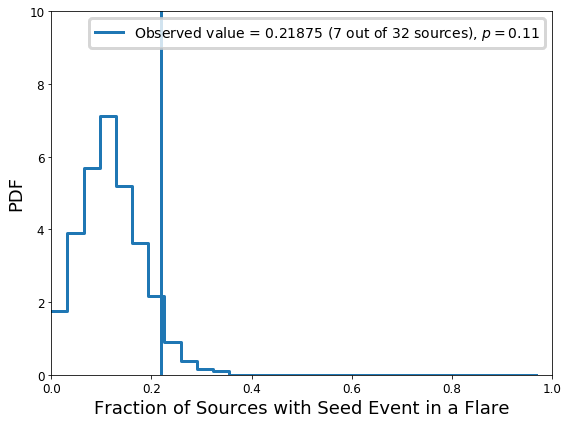
\includegraphics[width=0.8\textwidth]{figs/evtflarecorr.png}
\caption{The distribution of number of flare curves that have a temporal correlation between the high energy seed event, and a fitted flare, obtained from sets of data where the right ascension of events has been randomized. The observed value (7 out of 32 sources, or 21.9\%) is shown as a blue vertical line. 11\% of trials have more than 7 correlations between seed events and fitted flares.}
\label{fig:stresults}
\end{figure}

It is also potentially interesting to investigate the distributions of the parameters fit by the multi-flare likelihood. By comparing the observed distributions with those expected from background scrambles, we can check for inconsistencies of our data with the null hypothesis. 

\begin{figure}[h]
\centering
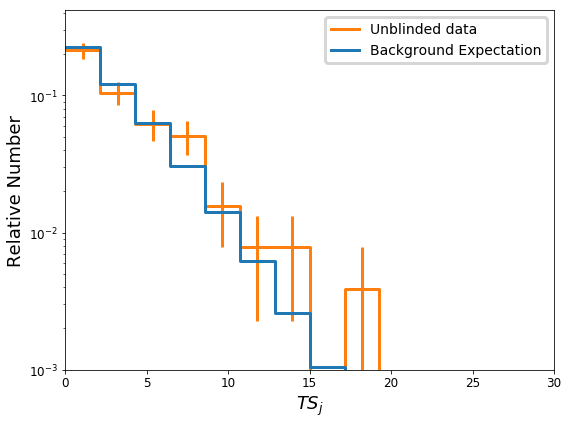
\includegraphics[width=0.4\textwidth]{figs/st_tsjdist.png}
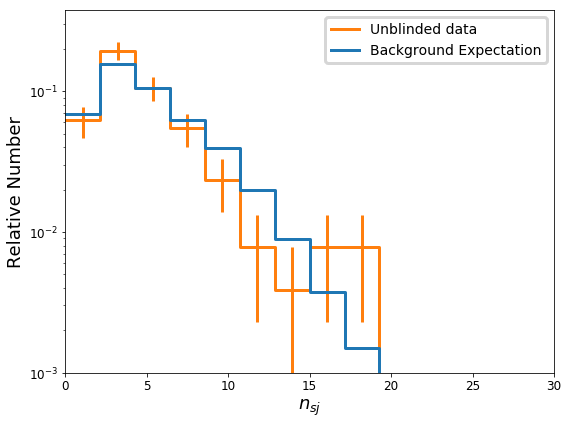
\includegraphics[width=0.4\textwidth]{figs/st_nsdist.png}
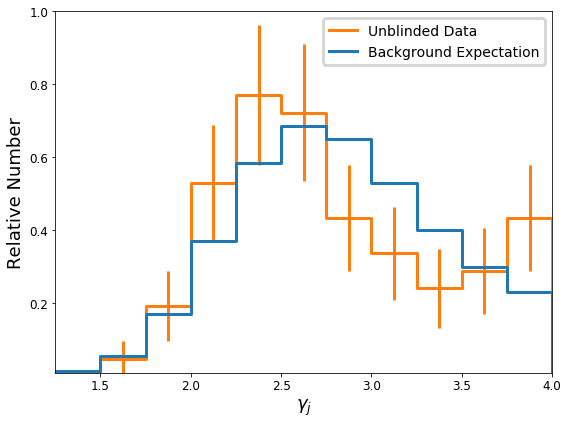
\includegraphics[width=0.4\textwidth]{figs/st_gammadist.png}
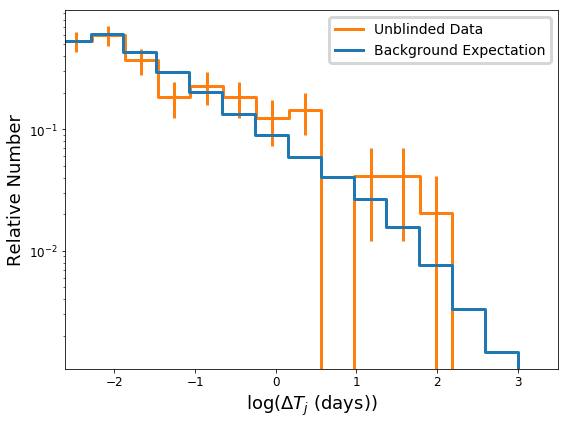
\includegraphics[width=0.4\textwidth]{figs/st_dtdist.png}
\caption{Distributions of fitted flare parameters for flares associated with the self-triggered catalog in both background scrambles (blue) and unblinded data (orange). While there is potentially some deformation in the distribution of fitted spectral indices (bottom left), a 2-sample K-S test comparing the observed and background distributions only returns a p-value of $p=0.26$, indicating that the blue and the orange distributions are not significantly inconsistent with one another. }
\label{fig:sthists}
\end{figure}

\section{Fermi 3LAC Blazars}
The 2014 TXS 0506+056 neutrino flare was notable not only for its association with a high energy IceCube alert, but also for its spatial coincidence with the blazar TXs 0506+056. In searching for additional neutrino sources, it is then not unreasonable to assemble a search for neutrino flares associated with a large catalog of blazars. For this purpose, we use the Fermi 3LAC catalog~\cite{fermi_3lac} to define a set of source candidates. Previous analyses searching for spatial coincidence with earlier iterations of this catalog have been performed, but were unable to identify any statistically significant excess~\cite{2lac_ic}. Here, we instead specifically search for transient emission using multi-flare algorithm described above. 

The Fermi 3LAC catalog is a catalog of AGNs detected by Fermi-LAT, consisting of gamma ray sources in the third Fermi-LAT catalog (3FGL)~\cite{fermi3fgl} between 100 MeV and 300 GeV with a Fermi test statistic greater than 25 between August 4, 2008, and July 31, 2012~\cite{fermi_3lac}. The catalog contains 1591 objects, the majority (98\%) of which are blazars, roughly evenly split between FSRQs and BL Lacs. Notably, TXS 0506+056 is a member of this catalog. 

In constructing this analysis, we select for blazars at declinations greater than $-5^{\circ}$, as the IceCube data sample (NorthernTracks v002p05) does not extend below this point. We impose no further cuts, and all sources are weighted equally when calculating a multi-flare test statistic. The equal weighting is chosen due to the unknown distribution of observed neutrino flare intensities, which is a combination of the redshift distribution and the unknown distribution of intrinsic neutrino flare intensities. Since this analysis seeks to be as model-agnostic as possible, no additional weighting scheme is implemented. The final catalog to be used for the multi-flare analysis consists of 1023 blazars, the locations of which are shown in figure~\ref{fig:3laccat}. This analysis is temporally untriggered, thus only the locations of the 3LAC blazars are used; since the multi-flare algorithm fits for the neutrino flare candidate duration purely from the neutrino data, no information from the gamma ray light curves for the source candidates is incorporated into this analysis. 

\begin{figure}[h]
\centering
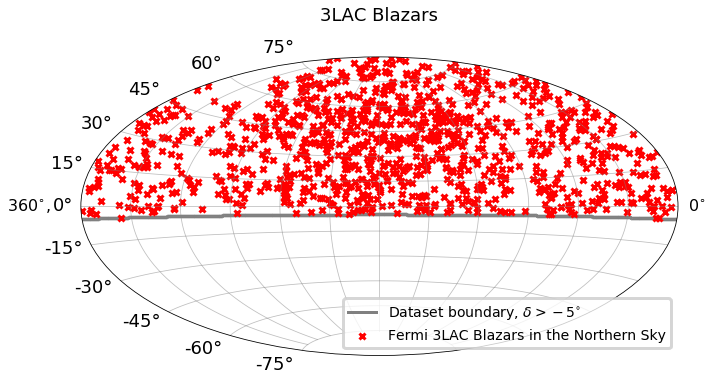
\includegraphics[width=0.8\textwidth]{figs/3lac_skymap.png}
\caption{The locations of the 3LAC blazars that compose the catalog used for a multi-flare analysis. Blazars with $\delta<5^{\circ}$ are not considered, as the IceCube NorthernTracks v002p05 data sample does not extend into this region. There are 1023 blazars that are considered as source candidates for the multi-flare analysis.}
\label{fig:3laccat}
\end{figure}

The results of applying the multi-flare algorithm to this catalog of 3LAC blazars can be summarized in figure~\ref{fig:3lacresults}. The optimization procedure for the most significant combination of sources returned a best fit number of sources of $k=125$, with an associated post-trial p-value of $p=0.06$. A list of these source candidates can be seen in table~\ref{tab:3lacresults}. As the significance of this excess is consistent with the null hypothesis, we do not claim discovery of neutrino flares associated with 3LAC blazars. 

Interestingly, despite the presence of the 2014 neutrino flare identified in~\cite{TXS_Archival}, TXS 0506+056 is not the most significant source candidate, having a pre-trial p-value of only $p=9.24 \times 10^{-3}$. This is not unexpected, considering that there does not appear to much activity (in terms of neutrino flares) at this location beyond the 2014 flare itself. As the multi-flare algorithm will return a high significance when there are multiple, moderately significant flares to stack together, it is unsurprising that there are other sources that have a higher multi-flare significance. As an example, the source candidate with the highest multi-flare significance is 1RXS J154604.6+081912. Rather than having a single large flare, the multi-flare algorithm fits multiple flares at this source candidate location, which combined have a significance of $p=8.1 \times 10^{-5}$, despite none of the individual flares having a local significance much greater than $p=0.01$.

\begin{figure}[h]
\centering
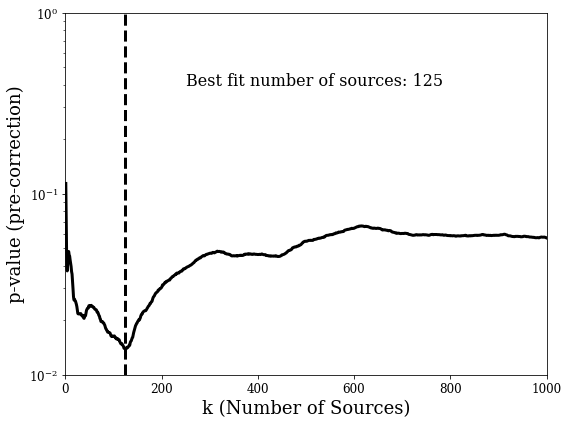
\includegraphics[width=0.4\textwidth]{figs/3lac_pcurve.png}
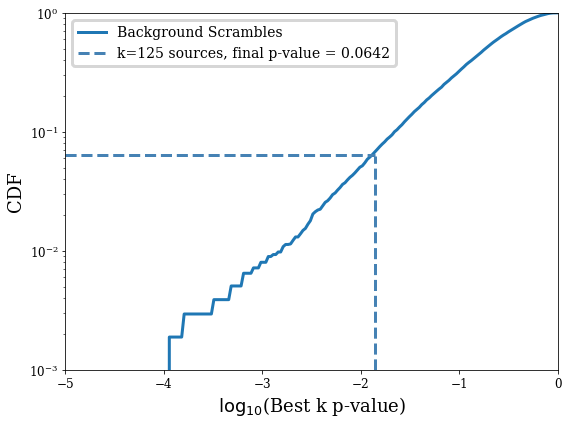
\includegraphics[width=0.4\textwidth]{figs/3lacresult.png}
\caption{Left: The local significance of stacking the $k$ highest test statistic sources in the 3LAC blazar catalog, as a function of $k$. The best fit value of $k=125$ can be seen as the minimum of this curve. Right: The trial corrected result for stacking the top 125 sources together, shown compared the background distribution obtained by applying the algorithm to right-ascension scrambled data. As the final p-value associated with the top 125 blazar sources is only $p=0.06$, there was no significant excess of neutrino flares observed to be associated with 3LAC blazars.}
\label{fig:3lacresults}
\end{figure}

Similar to the self-triggered catalog, we can additionally examine the distributions of the flare parameters that were fit for all the sources in the 3LAC catalog. No significant deviations from the background expectation are observed in any of the flare parameter distributions, as seen in figure~\ref{fig:3lacresults}.

As with the self-triggered catalog, we also obtain neutrino flare curves describing the historical variability of each source candidate. Figure~\ref{fig:3lacflarecurves} shows the flare curves of several 3LAC source candidates of note, including TXS 0506+056. While none of these sources are significant enough to claim discovery, flare curves like the ones shown here are a potentially valuable tool for multi-messenger analyses in the future that may seek to correlate neutrino emission with other astrophysical messengers. 

Though the application of the multi-flare algorithm to this catalog of 3LAC blazars did not result in a significant detection, it does allow us to constrain the behavior of neutrino flares associated with 3LAC blazars. Given that this method stacks flares together, the lack of a significant results suggest that there is an upper limit to how bright and numerous blazar neutrino flares may be. We express these limits in terms of the flare rate (how many flares occurred over the livetime of the data sample), and the per-flare $E^2$ flux. This allows us to compare to previously calculated limits obtained from a time-integrated analysis~\cite{2lac_ic}. These upper limits can be seen in figure~\ref{fig:3laclimits}

\begin{figure}[h]
\centering
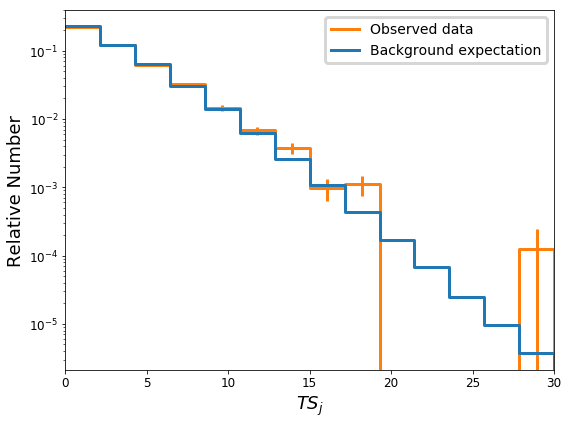
\includegraphics[width=0.4\textwidth]{figs/3lac_tsjs.png}
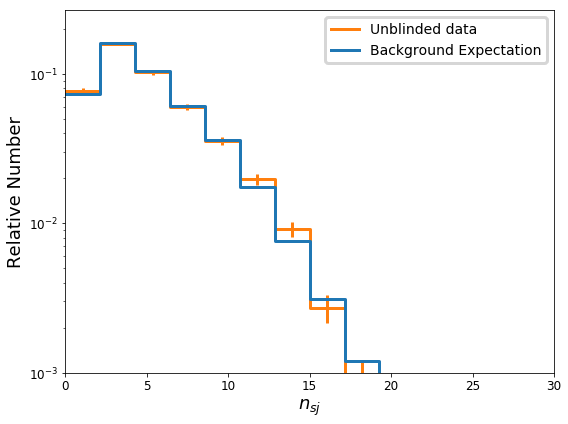
\includegraphics[width=0.4\textwidth]{figs/3lac_nss.png}
\includegraphics[width=0.4\textwidth]{figs/3lac_gammas.png}
\includegraphics[width=0.4\textwidth]{figs/3lac_dts.png}
\caption{Distributions of fitted flare parameters for flares associated with the 3LAC blazar catalog in both background scrambles (blue) and unblinded data (orange). All distributions of fit parameters from observed data appear to be consistent with the background expectation. As this catalog includes TXS 0506+056, the 2014 neutrino flare originally discovered in the IC170922A follow-up analysis~\cite{TXS_Archival} is visible as the rightmost entry in the histogram of flare $TS_j$ values in the plot in the upper left, having a value of $TS_j=27.9$. There are no other flares that were fit in this catalog with $TS_j>20$. }
\label{fig:3lacresults}
\end{figure}

\begin{figure}[h]
\centering
\includegraphics[width=0.44\textwidth]{figs/1RXS J154604.6+081912.pdf}
\includegraphics[width=0.44\textwidth]{figs/TXS 0506+056.pdf}
\caption{Neutrino flare curves for several sources of note in the multi-flare 3LAC blazar catalog analysis. The flare curves generated by the multi-flare algorithm are shown in blue, while the results of a corresponding single-flare analysis (that only fits the largest flare on each source) are shown in orange. Left: 1RXS J154604.6+081912, the most significant 3LAC blazar in the multi-flare analysis, having a pre-trial multi-flare p-value of $p=8.11 \times 10^{-5}$. Note that for this particular source, the multi-flare significance driven by a set of five moderately significant flares, none of which are particularly significant on their own. The significance of this source in the single-flare analysis was only $p=0.02$. Right: The flare curve for TXS 0506+056, showing the sizeable 2014 neutrino flare originally observed in~\cite{TXS_Archival}. The multi-flare p-value for TXS 0506+056 is only $p=9.24 \times 10^{-3}$, as other than the 2014 neutrino flare, there are no other particularly significant neutrino flare candidates at this location. }
\label{fig:3lacflarecurves}
\end{figure}

\begin{figure}[h]
\centering
\includegraphics[width=0.8\textwidth]{figs/3lac_lims.png}
\caption{The 90\% upper limits associated with the non-detection of a multi-flare signal using the 3LAC blazar catalog. The solid black line represents the time integrated limits obtained from ~\cite{2lac_ic}. Colored curves represent limits associated with various flare durations, as the multi-flare method imposes more stringent limits in the case that flares are shorter (for a fixed $E^2$ flux per flare). Note that the parameter space that is realistically accessible to a time-dependent analysis is somewhat compressed: points below the x-axis do not produce more than 1 flare in the data sample, on average, and points to the left of the vertical dashed line have an average flare size of $< 1$ event. The limits associated with flares with durations $\Delta t < 0.1$ days are expected to be similar to the limits associated with 0.1-day flares, as the improvement in sensitivity asypmtotes as the injected flare duration decreases.}
\label{fig:3laclimits}
\end{figure}


%\captionsetup{width=20cm}
\begin{center}
\label{tab:3lacresults}
\begin{longtable}{||cccccc||}
\caption{The top 125 multiflare source candidates in the 3LAC blazar catalog.}\\
\hline
Source Candidate Name & Source Class & RA (deg) & Dec (deg) & $\hat{n}_s$ & $p$ (pre-trial)\\
\hline
\endfirsthead
\multicolumn{6}{c}%
{\tablename\ \thetable\ -- \textit{Continued from previous page}} \\
\hline
Source Candidate & Source Class & RA (deg) & Dec (deg) & $\hat{n}_s$ & $p$ (pre-trial) \\
\hline
\endhead
\hline \multicolumn{4}{r}{\textit{Continued on next page}} \\
\endfoot
\hline
\endlastfoot
1RXS J154604.6+081912 &  bll  & 236.52 & 8.32 & 53.49 & 8.11e-5  \\
RBS 1467 &  bll  & 227.18 & 27.15 & 55.11 & 3.05e-4  \\
GB6 J0723+2859 &  fsrq  & 110.98 & 28.99 & 40.48 & 4.58e-4  \\
RBS 1558 &  bll  & 241.59 & 56.51 & 28.88 & 1.92e-3  \\
PMN J2324+0801 &  bll  & 351.19 & 8.04 & 28.15 & 3.11e-3  \\
B2 2214+24B &  bll  & 334.25 & 24.36 & 36.90 & 3.79e-3  \\
GB6 J0850+4855 &  bll  & 132.50 & 48.92 & 38.18 & 4.75e-3  \\
4C +20.25 &  fsrq  & 171.49 & 20.10 & 27.83 & 5.02e-3  \\
MG2 J094148+2728 &  fsrq  & 145.45 & 27.48 & 60.58 & 5.12e-3  \\
TXS 2241+406 &  bll  & 341.05 & 40.95 & 22.61 & 5.23e-3  \\
TXS 0213+619 &  bcu III  & 34.26 & 62.19 & 30.15 & 5.32e-3  \\
GB6 J0100+0745 &  bll  & 15.09 & 7.76 & 37.33 & 6.45e-3  \\
RX J0850.5+3455 &  bll  & 132.65 & 34.92 & 20.42 & 7.16e-3  \\
B2 1436+37B &  fsrq  & 219.72 & 37.18 & 49.47 & 7.83e-3  \\
MG1 J165034+0824 &  fsrq  & 252.66 & 8.41 & 39.19 & 7.83e-3  \\
PKS 0256+075 &  fsrq  & 44.86 & 7.79 & 42.53 & 9.04e-3  \\
TXS 0506+056 &  bll  & 77.36 & 5.69 & 20.71 & 9.24e-3  \\
1ES 1421+582 &  bll  & 215.66 & 58.03 & 28.49 & 0.0100  \\
TXS 0518+211 &  bll  & 80.44 & 21.21 & 48.49 & 0.0118  \\
W Comae &  bll  & 185.38 & 28.23 & 30.32 & 0.0123  \\
NVSS J141828+354250 &  bcu II  & 214.62 & 35.71 & 40.74 & 0.0128  \\
PKS 1532+01 &  fsrq  & 233.72 & 1.52 & 30.78 & 0.0131  \\
PKS 1424+240 &  bll  & 216.75 & 23.80 & 52.78 & 0.0148  \\
B3 2319+444 &  fsrq  & 350.58 & 44.76 & 41.93 & 0.0160  \\
PKS 0039+230 &  fsrq  & 10.52 & 23.33 & 48.89 & 0.0168  \\
B3 2238+410 &  bll  & 340.28 & 41.34 & 21.24 & 0.0175  \\
TXS 2315+189 &  bcu II  & 349.60 & 19.25 & 31.98 & 0.0197  \\
B3 2322+396 &  bll  & 351.32 & 39.96 & 30.07 & 0.0199  \\
NVSS J080637+774607 &  bcu II  & 121.66 & 77.77 & 52.32 & 0.0215  \\
MG1 J010908+1816 &  bll  & 17.28 & 18.27 & 26.59 & 0.0220  \\
1H 0323+342 &  nlsy1  & 51.17 & 34.18 & 10.09 & 0.0221  \\
NVSS J131921+775823 &  bcu II  & 199.84 & 77.97 & 16.99 & 0.0224  \\
RX J1351.3+1115 &  bll  & 207.84 & 11.25 & 27.93 & 0.0228  \\
RGB J1808+468 &  bll  & 272.00 & 46.83 & 29.19 & 0.0252  \\
RX J1149.5+2439 &  bll  & 177.38 & 24.66 & 33.52 & 0.0266  \\
TXS 2157+102 &  bll  & 330.03 & 10.50 & 47.04 & 0.0271  \\
S5 1357+76 &  fsrq  & 209.48 & 76.72 & 35.44 & 0.0274  \\
S5 1803+784 &  bll  & 270.19 & 78.47 & 27.73 & 0.0287  \\
GB6 J1439+4958 &  bll  & 219.95 & 49.97 & 32.32 & 0.0291  \\
B2 2234+28A &  bll  & 339.09 & 28.48 & 25.36 & 0.0298  \\
GB6 J0929+5013 &  bll  & 142.31 & 50.23 & 20.09 & 0.0306  \\
RGB J2054+002 &  bll  & 313.74 & 0.26 & 26.79 & 0.0315  \\
1ES 1028+511 &  bll  & 157.83 & 50.89 & 35.27 & 0.0333  \\
GB6 J0331+6307 &  bcu II  & 52.97 & 63.14 & 26.86 & 0.0335  \\
PKS 2320-035 &  fsrq  & 350.88 & -3.28 & 15.57 & 0.0350  \\
GB6 J0934+3926 &  bll  & 143.53 & 39.44 & 32.46 & 0.0352  \\
B2 1811+31 &  bll  & 273.40 & 31.74 & 35.37 & 0.0356  \\
GB6 J0937+5008 &  fsrq  & 144.30 & 50.15 & 27.81 & 0.0357  \\
TXS 1015+057 &  fsrq  & 154.62 & 5.51 & 19.30 & 0.0361  \\
TXS 1614+473 &  fsrq  & 243.92 & 47.19 & 16.66 & 0.0374  \\
4C +04.42 &  fsrq  & 185.59 & 4.22 & 19.22 & 0.0376  \\
MG2 J110606+2812 &  fsrq  & 166.53 & 28.21 & 41.99 & 0.0396  \\
RX J1246.9+4423 &  bll  & 191.75 & 44.39 & 22.30 & 0.0396  \\
B2 2308+34 &  fsrq  & 347.77 & 34.42 & 41.08 & 0.0408  \\
TXS 2106-030 &  bll  & 317.19 & -2.84 & 16.86 & 0.0410  \\
NVSS J125820+612049 &  bll  & 194.59 & 61.35 & 36.36 & 0.0425  \\
SBS 0812+578 &  bll  & 124.09 & 57.65 & 41.15 & 0.0426  \\
WN B1609.6+8517 &  bcu II  & 240.13 & 85.16 & 37.14 & 0.0434  \\
PMN J2227+0037 &  bll  & 336.99 & 0.62 & 28.56 & 0.0440  \\
1RXS J234332.5+343957 &  bll  & 355.89 & 34.66 & 25.27 & 0.0440  \\
GB6 J0529+0934 &  bcu II  & 82.26 & 9.58 & 32.69 & 0.0450  \\
MG2 J131037+2447 &  bcu III  & 197.66 & 24.81 & 27.71 & 0.0458  \\
3C 454.3 &  fsrq  & 343.49 & 16.15 & 37.56 & 0.0459  \\
GB6 J0929+7304 &  bcu II  & 142.43 & 73.07 & 25.62 & 0.0459  \\
ZS 0214+083 &  bll  & 34.32 & 8.62 & 36.08 & 0.0485  \\
3C 264 &  rdg  & 176.27 & 19.61 & 36.47 & 0.0485  \\
RXS J094620.5+010459 &  bll  & 146.58 & 1.08 & 19.50 & 0.0486  \\
NRAO 512 &  fsrq  & 250.12 & 39.78 & 21.52 & 0.0490  \\
1H 0323+022 &  bll  & 51.56 & 2.42 & 43.87 & 0.0494  \\
GB6 J1027+7428 &  bcu II  & 156.85 & 74.47 & 31.92 & 0.0495  \\
RX J0805.4+7534 &  bll  & 121.36 & 75.57 & 30.25 & 0.0505  \\
4C +73.07 &  bcu II  & 142.25 & 72.95 & 22.60 & 0.0514  \\
B3 1222+438 &  bll  & 186.21 & 43.59 & 28.13 & 0.0516  \\
MG1 J120448+0408 &  fsrq  & 181.22 & 4.14 & 33.72 & 0.0525  \\
GB6 J0148+5202 &  bcu III  & 27.08 & 52.03 & 19.63 & 0.0556  \\
7C 1823+6856 &  bll  & 275.89 & 68.96 & 21.57 & 0.0561  \\
MG2 J180948+2910 &  bll  & 272.44 & 29.17 & 34.89 & 0.0591  \\
NVSS J022304+682154 &  bcu II  & 35.77 & 68.37 & 31.49 & 0.0591  \\
OM 280 &  bll  & 177.58 & 24.30 & 42.49 & 0.0626  \\
PKS 1717+177 &  bll  & 259.80 & 17.75 & 24.64 & 0.0627  \\
1RXS J133021.4+444117 &  bll  & 202.59 & 44.69 & 22.24 & 0.0650  \\
S4 1726+45 &  fsrq  & 261.87 & 45.51 & 34.78 & 0.0664  \\
RX J1702.6+3115 &  bll  & 255.66 & 31.26 & 25.34 & 0.0664  \\
SBS 1410+530 &  bcu I  & 212.96 & 52.82 & 24.04 & 0.0666  \\
MG1 J154628+1817 &  bll  & 236.60 & 18.29 & 40.11 & 0.0668  \\
MG2 J190411+3627 &  bcu II  & 286.05 & 36.45 & 34.19 & 0.0713  \\
TXS 2331+073 &  fsrq  & 353.55 & 7.61 & 27.29 & 0.0731  \\
PKS 2047+098 &  bcu II  & 312.44 & 10.05 & 19.18 & 0.0734  \\
GB6 J1542+6129 &  bll  & 235.74 & 61.50 & 34.32 & 0.0736  \\
S5 0159+723 &  bll  & 30.89 & 72.55 & 30.54 & 0.0765  \\
TXS 2032+117 &  fsrq  & 308.65 & 11.91 & 21.51 & 0.0777  \\
S5 1027+74 &  bcu I  & 157.84 & 74.70 & 30.89 & 0.0777  \\
RGB J1426+340 &  bll  & 216.53 & 34.07 & 45.49 & 0.0778  \\
B3 0350+465 &  bcu III  & 58.63 & 46.72 & 22.88 & 0.0778  \\
RGB J1742+597 &  bll  & 265.63 & 59.75 & 37.12 & 0.0781  \\
1RXS J125117.4+103914 &  bll  & 192.82 & 10.65 & 18.18 & 0.0782  \\
MG3 J184126+2910 &  bcu II  & 280.34 & 29.16 & 37.55 & 0.0787  \\
TXS 1645+635 &  fsrq  & 251.49 & 63.50 & 36.91 & 0.0793  \\
B3 1058+413 &  bcu III  & 165.35 & 41.06 & 44.91 & 0.0799  \\
87GB 152947.5+574636 &  bll  & 232.74 & 57.61 & 21.01 & 0.0802  \\
GB6 J0229+6706 &  bcu III  & 37.34 & 67.11 & 11.03 & 0.0806  \\
MG1 J125348+0326 &  bll  & 193.45 & 3.44 & 27.69 & 0.0806  \\
GB6 J0342+3858 &  fsrq  & 55.57 & 38.99 & 33.59 & 0.0806  \\
PMN J0148+0129 &  bll  & 27.14 & 1.48 & 18.43 & 0.0818  \\
87GB 164812.2+524023 &  bll  & 252.35 & 52.59 & 33.97 & 0.0827  \\
GB6 J0024+0349 &  fsrq  & 6.19 & 3.82 & 31.06 & 0.0830  \\
B3 1307+433 &  bll  & 197.36 & 43.08 & 22.38 & 0.0839  \\
NVSS J092542+595812 &  bll  & 141.43 & 59.97 & 17.27 & 0.0913  \\
TXS 1549+089 &  bll  & 238.01 & 8.85 & 30.66 & 0.0915  \\
RX J0202.9-0223 &  bcu II  & 30.72 & -2.39 & 11.81 & 0.0922  \\
PKS 1203+04 &  ssrq  & 181.58 & 4.10 & 39.00 & 0.0926  \\
3C 221 &  rdg  & 143.78 & 39.70 & 28.81 & 0.0931  \\
RBS 0909 &  bll  & 162.86 & 39.72 & 30.20 & 0.0942  \\
NVSS J121500+500216 &  bll  & 183.75 & 50.04 & 36.18 & 0.0956  \\
RX J1101.3+4108 &  bll  & 165.35 & 41.15 & 39.73 & 0.0962  \\
OX 131 &  fsrq  & 320.25 & 19.02 & 28.54 & 0.0970  \\
PKS 0017+200 &  bll  & 4.91 & 20.36 & 25.43 & 0.0973  \\
1ES 0647+250 &  bll  & 102.69 & 25.05 & 33.94 & 0.0990  \\
TXS 0237+655 &  bcu II  & 40.34 & 65.72 & 22.76 & 0.102  \\
NVSS J224753+441317 &  bll  & 341.97 & 44.22 & 29.52 & 0.102  \\
OI 280 &  fsrq  & 117.72 & 12.52 & 22.89 & 0.102  \\
B2 1348+30B &  fsrq  & 207.72 & 30.58 & 27.45 & 0.102  \\
TXS 1833+137 &  bcu III  & 278.90 & 13.81 & 23.62 & 0.105  \\
RX J1027.4+6317 &  bll  & 156.85 & 63.30 & 31.32 & 0.105  \\
PKS 2354-021 &  bll  & 359.35 & -1.87 & 5.92 & 0.105  \\
\end{longtable}
\end{center}




\chapter{An All-Sky Multi-flare Analysis}\label{chapter:multiflareskymap}

\section{Motivation}
While the previous section outlined the application of the multi-flare algorithm to a pair of source catalogs, an additional obvious application of the method is to simply apply the algorithm across the entire neutrino sky. While catalog searches have the advantage of a greatly reduced trial factor, they also rely on having a mostly-correct guess of the underlying source population. By contrast, an all-sky search could potentially reveal sources without requiring any prior knowledge of what the specific sources could be, and could additionally even identify astrophysical neutrino sources with no multi-messenger counterpart. Given the results of a temporally untriggered neutrino flare associated with TXS 0506+056~\cite{TXS_Archival}, it is only natural to ask whether other such flares exist in IceCube's astrophysical neutrino data. An all-sky multi-flare analysis would be an appropriate approach of detecting a population of TXS-like flares, should they exist. 

Similar to the FAVA analysis produced by the Fermi collaboration~\cite{fava_paper}, an IceCube multi-flare skymap provides a description of the temporal variability of every point in the sky. Even in the absence of a statistically significant population of neutrino flares, these neutrino "flare curves" may be of use for multi-messenger analyses in the future, similar to what was done for TXS 0506+056~\cite{TXS_Archival}\cite{TXS_Multimessenger}.

\section{Analysis Construction}
Conceptually, the construction of an all-sky multi-flare analysis is fairly straightforward: a grid of pixels with  is defined over the entire sky using the \texttt{HEALPY} software package~\cite{healpy2019}. Using a \textt{HEALPY} grid with a \texttt{Nside=256} results in a grid of $786,432$ pixels, each with a radius of $0.12^{\circ}$. Pixels with declinations $\delta>85^{\circ}$ or $\delta<-85^{\circ}$ are excluded, as the data-driven method of estimating background using data scrambled in right ascension does not perform well in this region due to the small statistics of declination bands near the poles. The multi-flare algorithm is then applied to the central location of each pixel, resulting in a map of multi-flare test statistics, each associated with an individual pixel. 

The significance of each pixel can then be calculated by comparing the observed multi-flare test statistic to a distribution of similar test statistics obtained by applying the above procedure to maps of IceCube events that have had their right ascension locations randomized, providing a description of the null hypothesis. Pixels are divided into 40 declination bands, and for each declination band a chi-squared distribution is fit to the distribution of test statistics in that declination range. A pre-trial local significance for each pixel is calculated by comparing a particular pixel test statistic to the chi-squared distribution that was fit in the corresponding declination band. Once this has been done for every pixel, a map of multi-flare p-values has been obtained, describing the local multi-flare significance of every pixel in the sky.

Once a p-value map has been generated, several basic tests can be conducted. The most obvious test is to simply check if the most significant pixel is more significant than is expected from the background case (a "hotspot" test). A distribution of most significant multi-flare p-values is created by applying the procedure above to a set of background maps. The most significant pixel in the observed multi-flare map can then be compared to this distribution to obtain a final hotspot significance that has been trial-corrected for the all sky trial factor. As the event selection is different in the northern and southern skies, this process is conducted separately for declinations $\delta>-5^{\circ}$ and $\delta<-5^{\circ}$

Populations of multi-flare sources may also be tested for using a binomial test. A set of "spatially independent" local hotspots may be obtained by defining a list of all pixels that are at least $1^{\circ}$ away from a more significant pixel. The binomial test statistic p-value of the population test is then defined as (eq.~\ref{eq:bitest}):

\begin{equation}
    p(k) = \sum_{i=k}^{N_{eff}} \binom{N_{eff}}{i}p_k^i(1-p_k)^{N_{eff}-i}
    \label{eq:bitest}
\end{equation}

Here, $p(k)$ is correlated with the significance of observing $k$ hot spots with a p-value of $p_k$ or less, and $N_{eff}$ is the effective number of trials associated with the list of hot spots, chosen to produce proper containment of the final binomial p-values (e.g. a final binomial p-value of $p=0.1$ or less should only occur in 10\% of background trials). In this case, $N_{eff}=N_{pixels}$ produces proper containment. Hot spots are ordered by decreasing significance, and $k$ is varied to identify the most significant combination. The $p(k)$ associated with the best fit $k$ is then compared to a distribution of $p(k)$'s obtained in a similar manner from data scrambled in right ascension, resulting in a final post-trial binomial p-value. Like with the study of the most significant pixel, this process is conducted separately in the northern and southern skies. 

Since the multi-flare algorithm fits for every flare candidate at a particular pixel, it is trivial to extract the single-flare skymap results from this process as well. The procedure is almost identical to that which was outlined above, except instead of using the multi-flare test statistic at each pixel, the test statistic of the flare with the highest test statistic at each pixel is used. The hotspot and population tests then proceed as normal.

This particular analysis uses the PSTracksv003p02 data set.

\section{Results}
\subsection{Hotspots and Populations Analysis}
The multi-flare pre-trial p-value map can be seen in figure~\ref{fig:mfskymap}, with the locations of the brightest multi-flare pixels marked. The most significant locations identified by the multi-flare algorithm have pre-trial p-values of $p=9.2\times10^{-6}$, located at (RA, Dec)=$(145.02^{\circ}, 36.42^{\circ})$ and $p=3.5\times10^{-7}$, located at (RA, Dec)=$(126.21^{\circ}, -24.81^{\circ})$. These pre-trial p-values can be corrected to account for the all-sky trial factor using the process described above, resulting in post-trial p-values of $p=0.69$ for the northern sky hot spot and $p=0.06$ for the southern sky hot spot.

\begin{figure}[h]
\centering
\includegraphics[width=0.8\textwidth]{figs/skymap_withlabels.png}
\caption{The p-value map produced by applying the multi-flare algorithm to the entire neutrino sky between $-85^{\circ}<\delta<85^{\circ}$. The locations of the most significant multi-flare pixels in each hemisphere are shown as red "$\times$'s", while the locations of the most significant individual flares in each hemisphere are shown as red "$+$'s". The gray line denotes the boundary between what is considered the "northern" and "southern" sky by the IceCube data sample that was used. }
\label{fig:mfskymap}
\end{figure}

The flare curves for the multi-flare hotspots can be seen in figure~\ref{fig:mfhotspots}. Note that the multi-flare test statistic is a measure of the activity of a source integrated over the entire livetime of the data sample. While no individual flares that were fit at either the northern or southern hotspot are particularly significant on their own, the combination of many moderately significant flares is what makes these pixels the brightest multi-flare pixels in their respective hemispheres. 

\begin{figure}[h]
\centering
\includegraphics[width=0.4\textwidth]{figs/fcurve_mf_north.png}
\includegraphics[width=0.4\textwidth]{figs/fcurve_mf_south.png}
\caption{The flare curves returned by the multi-flare algorithm for the most significant pixel in the northern sky (left), and southern sky (right). For comparison, a complementary high-purity fit that uses a gaussian hypothesis and more stringent cuts on flare decorrelation is shown in orange. In both the northern and southern sky, the multi-flare significance is fueled not by individual flares with high local significance, but rather by a large number of moderately significanct flares. }
\label{fig:mfhotspots}
\end{figure}

Since the application of the high-statistics multi-flare analysis involves fitting every possible flare in the data, it is trivial to additionally calculate the significance of the largest individual flare candidate that was fit in both the northern and southern sky. We find that the most significant flare candidate in the northern sky is located at (RA, Dec)=$(21.97^{\circ}, -0.60^{\circ})$ (recall that the "northern sky" refers to declinations between $-5^{\circ}$ and $85^{\circ}$), and has a pre-trial significance of $p=5.08\times10^{-6}$ ($p=0.82$ post-trial). The most significant flare candidate in the southern sky is located at (RA, Dec)=($311.66^{\circ}, -18.84^{\circ}$), and has a pre-trial significance of $p=6.8\times10^{-6}$ ($p=0.53$ post-trial). 

\begin{figure}[h]
\centering
\includegraphics[width=0.4\textwidth]{figs/fcurve_sf_north.png}
\includegraphics[width=0.4\textwidth]{figs/fcurve_sf_north.png}
\caption{The flare curves returned by the multi-flare algorithm for the most significant flares identified in the northern sky (left), and southern sky (right). For comparison, a complementary high-purity fit that uses a gaussian hypothesis and more stringent cuts on flare decorrelation is shown in orange. Since neither of these locations appear to display significant activity beyond the large individual flares, these do not constitute particularly significant locations from a multi-flare perspective.}
\label{fig:mfhotspots}
\end{figure}

In addition to examining the most significant pixels that were seen, it is also informative to conduct a population analysis on the set of spatially independent ($>1^{\circ}$ separation) hotspots using the binomial test framework described above. In both the northern and southern sky, the binomial test was conducted for the set of spatially independent hotspots, defined by both the local multi-flare and single-flare significance. In all cases, the best-fit combination of hotspots was $k=1$, tagging only the most significant pixel, and none of the associated binomial p-values were significant (results may be viewed in table~\ref{tab:popresults}).

\begin{table}[h]
\centering
\begin{tabular}{ccccc}
    %\multicolumn{5}{c}{Results}\\
    \hline
    \hline
    Analysis & Search & Hemisphere & Pre-trial p-value & Post-trial p-value\\[3pt] \hline
    \multirow{4}{*}{Multi-flare} & \multirow{2}{*}{Hottest spot} & North & $9.2\times10^{-6}$ & 0.69\\ & & South & $3.5\times10^{-7}$ & 0.06 \\ \cline{2-5}  & \multirow{2}{*}{Population test} & North & 0.98 & 0.98\\ & & South & 0.12 & 0.12\\ [3pt] \hline
    \multirow{4}{*}{Single Flare} & \multirow{2}{*}{Hottest spot} & North & $5.08\times10^{-6}$& $0.82$\\ & & South & $6.70\times10^{-6}$& $0.53$\ \\ \cline{2-5}  & \multirow{2}{*}{Population test} & North & $0.88$ & $0.88$\\ & & South & $0.91$ & $0.91$ \\
    \hline
    \hline
\end{tabular}
\caption{Summary of the tests that were performed on the unblinded multi-flare skymap. Both hotspot and population analyses were conducted using both the local multi-flare significance (summing contributions from all flare candidates at a particular location) and the local single-flare significance (taking only the largest flare fit at each location). There were no significant transient neutrino sources identified by any of the tests conducted. }
\label{tab:popresults}
\end{table}

\begin{figure}[h]
\centering
\includegraphics[width=0.4\textwidth]{figs/bicurve_north.png}
\includegraphics[width=0.4\textwidth]{figs/bicurve_south.png}
\includegraphics[width=0.4\textwidth]{figs/bicurve_sf_north.png}
\includegraphics[width=0.4\textwidth]{figs/bicurve_sf_south.png}
\caption{The local significance of the binomial test for various values of $k$, the fitted number of hotspots, for both single and multi-flare binomial tests conducted in both the northern and southern hemispheres. Unblinded data is shown in red, while results obtained from background maps are shown in blue. In all cases using unblinded data, the observed binomial test curve has a global minimum at $k=1$, with an associated p-value that is consistent with the background expectation.}
\label{fig:bicurves}
\end{figure}

The results of the population analysis are unsurprising, given the distribution of per-pixel local p-values observed from the data. In the presence of a significant population of flaring neutrino sources, some deformation of the local p-value distribution should be visible, however as can be seen in figure~\ref{fig:pdists}, the observed distribution is entirely consistent with what is expected from background maps. 

\begin{figure}[h]
\centering
\includegraphics[width=0.4\textwidth]{figs/pixel_pdist_north.png}
\includegraphics[width=0.4\textwidth]{figs/pixel_pdist_south.png}
\includegraphics[width=0.4\textwidth]{figs/pixel_sf_pdist_north.png}
\includegraphics[width=0.4\textwidth]{figs/pixel_sf_pdist_south.png}
\caption{The local p-value distributions for the local multi-flare pixel significance (top) and the local single-flare pixel significance (bottom), for both data (red) and background maps (blue bands). In all cases, the observed distribution is consistent with the background expectation.}
\label{fig:pdists}
\end{figure}

Similar to the p-value distributions, the distributions of fitted flare parameters are also consistent with the background expectation, as can be seen in figure~\ref{fig:fitparamdists}. There does not appear to be a significant sub-population of transient sources with a particular flare duration, spectral index, flare rate, or flare flux. 

\begin{figure}[h]
\centering
\includegraphics[width=0.4\textwidth]{figs/fitted_flare_durations.png}
\includegraphics[width=0.4\textwidth]{figs/fitted_flare_gamma.png}
\includegraphics[width=0.4\textwidth]{figs/fitted_flare_Nflare.png}
\includegraphics[width=0.4\textwidth]{figs/fitted_flare_ns.png}
\caption{Distributions of fitted flare parameters: flare duration (top, left), spectral index (top, right), number of flares fit at a particular candidate location}
\label{fig:fitparamdists}
\end{figure}

The observed diffuse astrophysical neutrino flux~\cite{stettner2019measurement} places restrictions on how bright and numerous neutrino flares may be. The non-detection of a population of transient astrophysical neutrino sources can be used to further constrain this space. These limits can be seen in figure~\ref{fig:mfskylim}, which shows 90\% upper limits on source flare rate and burst energy in neutrinos, as well as limits that can be placed on the per-source flare rate. Note that these limits are a statistical statement about the data itself: If the "true" parameters describing a population of transient neutrino sources lies above these lines, the data would have had a larger population of significant flares than what was observed. 

\begin{figure}[h]
\centering
\includegraphics[width=0.4\textwidth]{figs/flarelims.png}
\includegraphics[width=0.4\textwidth]{figs/sourceratelims.png}
\caption{Left: 90\% upper limits on neutrino source density and per-source flare rate obtained from the all-sky multi-flare analysis. In this plot, transient sources are assumed to compose 100\% of the astrophysical neutrino flux, with the FIRESONG simulation package~\cite{firesong_ref} being used to distribute the flux among sources according to the Hopkins and Beacom (2006) source evolution model~\cite{Hopkins_2006}. Flares are simulated to have a duration of 20 days, and a spectral index of $\gamma=2.28$. All flares on the same source are assumed to have the same intrinsic intensity, equal to the time integrated source flux divided by the number of flares. Right: The 90\% upper limits on the source rate (source density $\times$ flare rate) as a function of neutrino burst energy. Blue lines correspond to combinations of source rate and neutrino burst energy that reproduce specific fractions of the diffuse astrophysical neutrino flux. In both plots, the parameters associated with several candidate source populations are shown for comparison..}
\label{fig:mfskylim}
\end{figure}


\subsection{Locations of External Interest}
Though this analysis was designed to be spatially untriggered (scanning over the entire sky, rather than the locations of a select few sources), the neutrino "flare curves" produced are a potentially powerful tool for exploring the historical behavior of source candidates identified though other methods. The skymap produced here is similar to the TXS 0506+056 followup analysis~\cite{TXS_Archival}, except that this analysis has now been performed at almost every location in the sky. This allows for easy followup of external triggers, as identifying potential transient neutrino emission associated with a source candidate is as easy as examining the flare curve at that location in the sky. 

To demonstrate the use of the all-sky flare curve map produced here, we examine the flare curves of several time-integrated source candidates identified by~\cite{10yr_tint} in order to explore the potential of temporally clustered neutrino emission from these locations. 

\subsubsection{NGC 1068}

The most significant location identified by the all-sky time-integrated analysis is spatially coincident with the Seyfert II galaxy NGC 1068. This source was also tested as part of a catalog of 110 candidate neutrino emitters, and was the brightest object in the catalog, with an associated post-trial significance of $2.9 \sigma$~\cite{10yr_tint}. These significances all arise from time-integrated tests that do not take into account the arrival time of the contributing neutrino events. It is then potentially interesting to explore the temporal structure of this excess with the flare curves that were produced as part of the multi-flare skymap. 

The flare curve generated at the location of NGC 1068 can be seen in figure~\ref{fig:ngc1068}. Though this location is significant under the time-integrated analysis, the multi-flare p-value is only $p=0.016$ (pre-trial), with no individual flare candidate having a local significance greater than $p=0.072$. Note however, that these results are not in tension with the time-integrated significance, as the time-integrated analysis tests only for an excess of events over the entire livetime of the sample. By contrast, a source with high multi-flare significance requires that events not only be clustered spatially, but temporally as well. As such, sources with high time-integrated significance do not necessarily have a correspondingly high multi-flare significance, particularly if there is not significance temporal clustering of events that contribute to the time-integrated result. 

Nonetheless, we have here provided a description of the historical behavior of the neutrino emission associated with NGC 1068. Despite the time-integrated excess observed in previous analyses, there does not appear to be significant temporal clustering of events at this location.

\subsubsection{Other Time-Integrated Candidates: PKS 1424+240  and GB6 J1542+6129}
In addition to identifying NGC 1068 as a potential source candidate, the population analysis component of the time integrated analysis~\cite{10yr_tint} also identified an excess of $3.3 \sigma$ associated with the combination of the sources NGC 1068, TXS 0506+056, PKS 1424+240, and GB6 J1542+6129. Figure~\ref{fig:othertints} shows the flare curves that were obtained at the locations of PKS 1424+240 and GB6 J1542+6129. 

Similar to NGC 1068, PKS 1424+240 does not display significant temporal clustering of neutrino events, and has a local multi-flare p-value of $p=0.085$. By contrast, GB6 J1542+612 seems to have a somewhat significant flare candidate beginning at MJD=57564.878 and ending at MJD=57944.512. The pre-trial significance of this flare candidate alone is $p=0.00173$ ($2.9 \sigma$). Combining all the flares candidates at the location of GB6 J1542+612 using the multi-flare test statistics results in a local multi-flare significance of $p=0.0098$ ($2.3 \sigma$). While this is not particularly significant (especially when the all-sky trial factor is considered), it does inform us that the period between MJD=57564.878 and MJD=57944.512 was likely a large contributor to the time-integrated significance for this particular source. If there are further multi-messenger signals from this location in the future, the neutrino flare candidates at this location may become of interest. 

\begin{figure}[h]
\centering
\includegraphics[width=0.8\textwidth]{figs/fcurve_NGC1068.png}
\caption{The flare curve at the location of NGC 1068, a source candidate that was identified as potentially interesting in the time-integrated analysis~\cite{10yr_tint}. While this is the brightest spot in the time-integrated analysis, the multi-flare analysis does not reveal any significant temporal clustering of events at this location, resulting in a local multi-flare significance of $p=0.016$}
\label{fig:ngc1068}
\end{figure}

\begin{figure}[h]
\centering
\includegraphics[width=0.4\textwidth]{figs/fcurve_PKS1424+240.png}
\includegraphics[width=0.4\textwidth]{figs/fcurve_GB6.png}
\caption{The flare curves at the locations of PKS 1424+240 and GB6 J1542+612. While PKS 1424+240 does not display any significant temporal clustering (having a local multi-flare p-value of $p=0.085$), GB6 J1542+612 has a potentially interesting flare candidate beginning at MJD=57564.878 and ending at MJD=57944.512. This flare candidate has a local flare significance of $p=0.00173$ ($2.9 \sigma$), contributing to the overall pre-trial multi-flare significance for GB6 J1542+612 of $p=0.0098$ ($2.3 \sigma$). }
\label{fig:othertints}
\end{figure}

\subsubsection{TXS 0506+056}
In addition to being part of the excess that was identified in the all-sky time-integrated analysis, TXS 0506+056 is notable for both the multi-messenger coincidence sparked by the high energy IceCube alert IC-170922A~\cite{TXS_Multimessenger}, as well as the archival analysis that revealed a $3.5 \sigma$ neutrino flare that occurred in 2014, prior to the 2017 high energy alert event~\cite{TXS_Archival}.

The all-sky multi-flare analysis presented in this work includes the location of TXS 0506+056, and we can consequently generate a flare curve for this source candidate. The flare curve observed in the all-sky multi-flare analysis can be seen in figure~\ref{fig:fcurve_txs}. TXS 0506+056 has a local multi-flare significance of $p=3.37 \times 10^{-4}$ ($3.4 \sigma$), with the main contributor being the 2014 neutrino flare candidate, beginning on MJD=56927.86 and ending on MJD=57072.99.

Readers who have been paying close attention to the content of this thesis (a group which at this point probably includes my thesis committee and like, no one else) may notice that the flare curve shown in figure~\ref{fig:fcurve_txs} seems to be in disagreement with the published result with regards to the 2014 TXS flare . While the result shown in~\cite{TXS_Archival} reports a significance for the 2014 flare candidate of $3.5 \sigma$, the all-sky multi-flare analysis presented here observes a local significance for this flare of only $p=0.0054$ ($2.5 \sigma$).

The difference in significance between the two results can be explained by the different event selections that were used in each analysis. Descriptions of these event samples may be found in section 3 of this thesis. While ~\cite{TXS_Multimessenger} used the PointSourceTracks v002p03 event sample, the all-sky multi-flare analysis presented here uses the PointSourceTracks v003p02 event sample. The most relevant difference between the two event samples in this case are the pre-cuts: PointSourceTracks v003p02 introduces a cut prior to the event selection BDT that requires events to have a reconstructed track length greater than 200 meters. This pre-cut does not exist in PointSourceTracks v002p03. 

\begin{figure}[h]
\centering
\includegraphics[width=0.8\textwidth]{figs/fcurve_TXS.png}
\caption{The flare curve obtained from the all-sky multi-flare analysis for TXS 0506+056. The pre-trial multi-flare significance of this location is $p=3.37 \times 10^{-4}$ ($3.4 \sigma$). Interestingly, the 2014 flare candidate is not seen at the original significance of $3.5 \sigma$ that was reported in ~\cite{TXS_Multimessenger}. While the 2014 flare candidate is present, this analysis obtains an associated local significance of only $p=0.0054$ ($2.5 \sigma$). }
\label{fig:fcurve_txs}
\end{figure}

\begin{figure}[h]
\centering
\includegraphics[width=0.45\textwidth]{figs/125659.png}
\includegraphics[width=0.45\textwidth]{figs/125762.png}
\caption{The two cascade-like events (event IDs: 40914587 and 56262988) that contributed to the 2014 TXS 0506+056 neutrino flare candidate in PointSourceTracks v002p03, but are not present in PointSourceTracks v003p02. The red arrows show the directional reconstruction assocaited with the track reconstruction that was used, however given the cascade topology of these events, this reconstruction is likely to be inaccurate. }
\label{fig:missingevts}
\end{figure}

As a result of the track length precut that was introduced in PointSourceTracks v003p02, two events (referred to by their event IDs: 40914587 and 56262988) that were major contributors to the 2014 TXS 0506+056 neutrino flare candidate were removed. These events have a cascade-like topology, though in PointSourceTracks v002p03, they are reconstructed as if they were tracks, leading to potentially inaccurate descriptions of the event direction and energy. Since these events are cascade-like, they have a short reconstructed track length, and as such these events do not exist in PointSourceTracks v003p02. 

Manually removing the two cascade events from the PointSourceTracks v002p03 data sample and recomputing the significance of the 2014 TXS 0506+056 neutrino flare results in a drop in significance comparable to what was seen when using PointSourceTracks v003p02, as can be seen in table~\ref{tab:TXSCrossChecks}. The drop in significance cannot be otherwise adequately explained by changes to the angular reconstruction or other differences between the two versions of the data sample. The time-integrated sensitivity of the two samples is comparable, and favors PointSourceTracks v3 at the declination of TXS 0506+056. As such, the drop in significance of the 2014 TXS 0506+056 flare candidate is unlikely to have been caused by PointSourceTracks v003p02 being an overall less sensitive sample.

\begin{table*}[h]
\centering
\begin{tabular}{cccccc}
\multicolumn{6}{c}{Untriggered Flare Cross-check Results} \\[0.1cm]
\hline
\hline
Sample & $p$ (pre-trial) & $T_\text{start}$ & $T_\text{stop}$ & $n_s$ & $\gamma$ \\ 
\hline
\texttt{PSTracks v2}~\cite{TXS_Archival} & 7.0e-5 & 56937.81 & 57096.22 & 14.39 & 2.20  \\
\texttt{PSTracks v2} w/o cascades & 1.17e-3 & 56937.81 & 57112.65 & 12.22 & 2.26 \\
\texttt{PSTracks v3} (multi-flare skymap) & 5.4e-3 & 56927.86 & 57072.99 & 11.87 & 2.22\\
\hline
\hline
\end{tabular}
\caption[]{The results of repeating the untriggered flare analysis preformed in~\cite{TXS_Archival}, but using {\tt PSTracks v3} in place of {\tt PSTracks v2}, the dataset that was originally used. The apparent drop in significance when using {\tt PSTracks v3} can be explained by cascade-like events present in {\tt v2} that have been removed from {\tt v3}.}\label{tab:TXSCrossChecks}
\end{table*}


\begin{figure}[h]
\centering
\includegraphics[width=0.8\textwidth]{figs/v2v3_senscompare.pdf}
\caption{A comparison of the time integrated sensitivities of PointSourceTracks v002p03 and PointSourceTracks v003p02. At the declination of TXS 0506+056 ($\delta=5.7^{\circ}$), PointSourceTracks v003p02 has a slightly better sensitivity. }
\label{fig:fcurve_txs}
\end{figure}

It should be noted that the result published in~\cite{TXS_Archival} is not incorrect, despite using an older data sample that contains unforseen background events. Since the methods used for the original untriggered flare analysis use a data-driven background estimation, the cascade background in PointSourceTracks v002p03 is accounted for in the original $3.5 \sigma$ significance that was reported for the 2014 neutrino flare candidate. 

Though the cascade background is handled differently in the PointSourceTracks v002p03 analysis versus the PointSourceTracks v003p02 analysis, the two results are not inconsistent with one another. Figure~\ref{fig:v2v3diff} shows the results of comparing the results of simulated flares comparable to the 2014 TXS flare injected into both PointSourceTracks v002p03 and PointsourceTracks v003p02.   As the background test statistic distributions for both samples are similar, comparing the test statistic values obtained using each sample is a good proxy for comparing the flare local significance.  For this test, trials of simulated signal at the location of TXS 0506+056 were injected into background maps generated using PointSourceTracks v002p03. The injected signal was chosen to replicate the best fit parameters in the original PointSourceTracks v002p03 untriggered flare analysis~\cite{TXS_Archival}: 13 events with a spectral index of $\gamma=2.2$, injected over a time window of length $\Delta t = 158$ days. A test statistic for each of these PointSourceTracks v002p03 signal trials was then calculated. The same simulated signal events were then injected into background trials generated with PointsourceTracks v003p02, but any events that do not pass the PointSourceTracks v003p02 event selection were removed.  A new PointSourceTracks v003p02 test statistic is then calculated for each of these trials with injected signal. 

Figure~\ref{fig:v2v3diff} shows the results of this crosscheck, showing the distribution of test statistics differences between the v2 and v3 test statistics. While on average the test statistic associated with a signal of this type is higher in PointSourceTracks v003p02, the distribution is rather wide, and it is not uncommon for the PointSourceTracks v003p02 result to be lower significance than the PointSourceTracks v002p03 result. A drop in significance comparable or greater than what was seen in the observed v2 and v3 results ($TS_{v3}-TS_{v2}=11.84$) occurs in 8\% of the simulated trials. 


\begin{figure}[h]
\centering
\includegraphics[width=0.4\textwidth]{figs/v2v3tsdists.png}
\includegraphics[width=0.4\textwidth]{figs/v2v3tsdiff.png}
\caption{Simulated trials comparing the significance of a flare comparable to the 2014 TXS 0506+056 flare in both PointSourceTracks v002p03 and PointSourceTracks v003p02. Left: the test statistic distributions for both datasets in the background (solid) and injected signal (dotted) cases. The PointSourceTracks v003p02 signal is identical to the PointSourceTracks v002p03 signal, except with events that do not pass the v3 selection removed. Right: A comparison of the v2 and v3 test statistics for each simulated signal trial, with the observed test statistic difference plotted as a vertical line. A drop in significance at least as large as what was seen in observed data occurs in 8\% of simulated trials.}
\label{fig:v2v3diff}
\end{figure}

While there appears to be a drop in significance for the 2014 TXS 0506+056 untriggered neutrino flare when using to the newer PointSourceTracks v003p02 data sample, it is important to realize that the updated v3 result is not inconsistent with the previous v2 result. Additionally, the 2014 flare composes only part of the ensemble of results that make TXS 0506+056 and interesting source candidate, as it is the combination of the 2014 untriggered neutrino flare with the 2017 high energy alert event and multi-messenger observations that suggest TXS 0506+056 as a source of astrophysical neutrinos. The significance of the 2014 TXS 0506+056 flare will likely continue to be monitored as the IceCube collaboration improves its data samples and reconstruction techniques, hopefully converging on a more precise measurement to the flare significance. 



\chapter{Outlook}\label{chapter:outlook}

In this work, we have introduced a novel method for fitting ensembles of neutrino flare candidates at a particular source location. This method was applied to two catalogs of source candidates motivated by TXS 0506+056: a catalog of northern-sky 3LAC blazars, and a "self-triggered" catalog of high energy IceCube events. Though neither catalog displayed a significant excess of neutrino flares, this allowed us to further constrain potential transient neutrino emission from blazars. 

The multi-flare algorithm introduced here was also applied on an all-sky scale. No significant population of neutrino flares was observed, though flare curves were produced at every location in the sky, providing a potentially useful tool for future multi-messenger searches wishing to incorporate information on the historical neutrino emission from source candidate locations, similar to what was done in~\cite{TXS_Archival}. 

The non-detection of a significant population of transient neutrino sources is somewhat interesting from the perspective of constraining astrophysical neutrino source populations. Whatever the sources of astrophysical neutrinos may be, they cannot produce neutrino flares that are so bright or numerous that the data becomes inconsistent with the background expectation on an all-sky scale. This places limits on the source density, flare rate, and neutrino burst energy that are not associated with any particular source class, serving as a "universal limit" of sorts on the behavior of potential astrophysical neutrino transients, as can be seen in figure~\ref{fig:mfskylim}. 

It should be noted, however, that a non-detection of neutrino sources on an all-sky scale is not entirely unexpected. The all-sky trial factor is quite large, and the most significant neutrino source candidates to date (TXS 0506+056 and NGC 1068) were both originally identified in spatially triggered analyses, where the candidate location was already identified as potentially interesting by other astrophysical messengers. Future, spatially triggered searches may be sensitive to individual sources that have been obscured by the all-sky trial factor. Ideally, the neutrino flare curves introduced in this work would aid with this, as the historical neutrino information provides an additional piece to the multi-messenger puzzle. 

Though the first applications of the multi-flare algorithm did not yield any significant discovery of astrophysical neutrino sources, the future of neutrino astronomy is still quite bright. With two interesting source candidates already identified, the answer to the question of the source of astrophysical neutrinos (and consequently, the source of high energy cosmic rays) is potentially beginning to become more clear. The upcoming years bring improvements to the IceCube detector calibration and event reconstruction, providing a more accurate description of existing data, as well as the construction of IceCube Gen2 which will boast increased effective area at high energies, thereby reducing the atmospheric neutrino background. Additionally, upcoming radio-based neutrino experiments such as RNO-G~\cite{RONG_design}, BEACON~\cite{Wissel_2020}, IceCube Gen2-Radio~\cite{Gen2paper}, PUEO~\cite{abarr2021payload}, and POEMMA~\cite{olinto2021poemma} will provide a view into the ultra-high energy neutrino regime, beyond what the current iteration of IceCube is realistically capable of measuring. As the identification of candidate neutrino emission from TXS 0506+056 was triggered by a single high energy neutrino event, the expansion of neutrino detectors into the high energy regime could lead the way to identifying future neutrino sources. 



\chapter{Appendix: Statistics Background}\label{chapter:stats}

Much of the material presented in this thesis requires an understanding of a few key areas of statistics. This material is typically covered in almost any introductory level statistics course, but is generally not part of the standard undergraduate physics curriculum. For this reason, I've collected some of the key concepts in this section, to potentially serve as a starting point for people who may not already be familiar with the statistical underpinnings of recent source searches in neutrino astronomy. An interactive ipython notebook showing examples of these concepts can also be found as part of the materials for the 2019-2021 IceCube bootcamps\footnotemark.

\footnotetext{https://events.icecube.wisc.edu/event/105/contributions/1054/}

\section{Estimators}
An estimator is a procedure applied to the data sample which gives a numerical value for a property of the parent population, or, as appropriate, a property or parameter of the parent distribution function.

This is a general definition: The sample of interest may have been drawn from a large parent population, for which some property is to be inferred. Alternatively, it may have been generated from a distribution function, arising from a basic law being investigated. This distribution function also has parameters and properties, which one may also wish to calculate (e.g. $\sigma$ for a 1 dimensional gaussian distribution).

Estimators are generally not classified as "right" or "wrong", rather we tend to classify estimators as "good" or "bad" based on their properties. Some properties that are often relevant when describing estimators:

\begin{itemize}
    \item An estimator is \textit{consistent} if it tends to the true value as the number of data values tends to infinity.
    \item An estimator is \textit{unbiased} if its expectation value is equal to the true value.
    \item An estimator is \textit{efficient} if its variance is small.
\end{itemize}

Estimators can be any number of the above, but good estimators should fulfill all three descriptions \cite{barlow_1989}. 

\section{Likelihoods}
One class of estimators that is commonly used in neutrino astronomy are \textit{likelihood-based estimators}. For a set of data, {$x_1, x_2, x_3 ...x_N$} produced from some underlying distribution with parameter $a$, the probability of obtaining that particular data set is the product of the individual probabilities of obtaining each of the $x_i$. This product is referred to as the *likelihood* (eq. \ref{likelihoodeq1} and \ref{likelihoodeq2}):

\begin{equation}
    L(x_1, x_2, x_3..x_N, a) = P(x_1;a)P(x_2;a)...P(x_N;a)
\label{likelihoodeq1}
\end{equation}

\begin{equation}
    L(x_1, x_2, x_3..x_N, a) = \prod_{i=1}^N P(x_i;a)
\label{likelihoodeq2}
\end{equation}

The likelihood is typically used to fit the model parameter $a$, given some observed data {$x_1, x_2, x_3 ...x_N$} by finding the value of $a$ which maximizes the likelihood function. Note that $a$ can be a vector of values in the case that we have a model with multiple free parameters. For computational reasons, the process of maximizing the likelihood is oftentimes done by minimizing the negative log-likelihood instead. Taking the logarithm of the likelihood function turns the product into a sum, making the derivative more intuitive and easier to work with numerically, and the switch from maximization of the likelihood to minimizing the negative likelihood is purely convention. 

\section{Confidence Intervals}
Suppose we want to know the value of a parameter $X$ and have estimated it from the data, giving result $x$. We know the resolution of our underlying distribution, and thus the variance, $V(x)$ and the standard deviation $\sigma$. Our goal is then to create a "confidence interval": An interval within which there is a $C$ \% chance that a single observation will lie within the interval, where $C$ is our "confidence level". Formally, the confidence interval ($x_-, x_+$) for a given confidence level $C$ obeys the requirement that (eq. \ref{confidenceinterval}):

\begin{equation}
    Prob(x_- \leq x \leq x_+) = \int_{x_-}^{x_+}P(x)dx = C
    \label{confidenceinterval}
\end{equation}

There are a few possible ways to construct this interval:

\begin{enumerate}
    \item The \textbf{symmetric interval}: $x_-$ and $x_+$ are equidistant from the mean, $\mu$, i.e $x_+ - \mu = \mu - x_-$
    \item The \textbf{central interval}: The probability above and below the interval are equal: $\int_{-\infty}^{x_-} P(x)dx = \int_{x^+}^{\infty} P(x)dx = (1-C)/2$
\end{enumerate}

Common values for $C$ are 68\% (1 $\sigma$), 90\% (1.64 $\sigma$), and 99\% (2.58 $\sigma$). There is a trade off between a narrow interval and low confidence. You can say with great confidence that a value will lie within a very wide interval, but if one wants to tie it down more precisely the confidence lessens. 

\section{Hypothesis Testing}
Many problems in science can be reduced to attempting to distinguish between 2 distinct possibilities, where the observed data has different properties under each. In many cases, we are attempting to distinguish between a "null hypothesis", which is used to refer to a "default" model (e.g. the absence of neutrino point sources), and an "alternative hypothesis", which represents the addition of some new physics, model parameter, or disagreement with the "default" case (e.g the presence of neutrino point sources). Statistical hypothesis testing is a framework for comparing these two hypotheses, given some set of observed data.

We can roughly break down the process of hypothesis testing into the following steps:

\begin{enumerate}
    \item State relevant null and alternative hypotheses
    \item State the test statistic
    \item Derive the distribution of the test statistic under the null hypothesis
    \item Select significance level ($\alpha$) at which the null hypothesis will be rejected
    \item Compute an observed test statistic from the data
    \item Calculate a p-value and decide whether to reject the appropriate hypothesis
\end{enumerate}

\subsection{State relevant null and alternative hypotheses}
When constructing an analysis, we should be careful to state the null and alternative hypotheses. Typically, the null hypothesis ($H_o$) refers to a statement or default position that there is no relationship between two phenomena, that there is no signal, or that our current models describe the data well. The alternative ($H_a$) hypothesis usually describes the opposite: that there is a relationship between two phenomena, that there is a signal, or that our models to NOT describe the data well. Here are some example pairs of hypotheses one might encounter when working with IceCube data:

\begin{itemize}
    \item $H_o$: Neutrino event arrival directions are not significantly correlated with the positions of blazars identified in Fermi's 3FGL catalog
    \item $H_a$: Neutrino event arrival directions are correlated with the positions of blazars identified in Fermi's 3FGL catalog
\end{itemize}

\begin{itemize}
    \item $H_o$: A 3-flavor oscillation model describes the IceCube data well
    \item $H_a$: IceCube data is inconsistent with a 3-flavor model
\end{itemize}

It is important to be careful when formulating null and alternative hypotheses so as to not overreach with the claims being made should the alternative hypothesis be accepted. In general, it's best to keep in mind the specifics of how a particular analysis is being constructed, and what the property of the data being measured actually is. For example, in the first pair of hypotheses above, it would be improper for our alternative hypothesis to be "blazars are a source of astrophysical neutrinos" if we were only examining the positions of the 3FGL catalog, which covers only a subset of all observed blazars. 

\subsection{State a test statistic}
A \textit{test statistic} is a quantity derived from the sample, intended to be a numerical summary of a dataset that reduces the data to one value that can be used for hypothesis testing. In general, the test statistic is selected in such a way as to quantify, within observed data, behaviors that would distinguish the null and alternative hypotheses. These are very similar to estimators, and we can oftentimes use estimators as test statistics. 

An important property of the test statistic is that its sampling distribution under the null hypothesis must be calculable either exactly or approximately. There are many types of test statistics that you can use, and what the exact form of the test statistic is will usually be determined by your analysis. One example of a test statistic is the chi-squared test statistic intended to compare counts in an oscillation analysis (eq. \ref{chi2eq}):

\begin{equation}
    \chi^2 = \sum_{i \in {bins}} \frac{(n_i^{\nu+\mu_{atm}} - n_i^{data})^2} {(\sigma_i^{data})^2+(\sigma_{\nu+\mu_{atm,i}})^2} 
    \label{chi2eq}
\end{equation}

Where $\chi^2$ is the test statistic, $i$ refers to bins in zenith and azimuth, $n_i^{\nu+\mu_{atm}}$ and $n_i^{data}$ are the number of events in a particular bin in both simulation and data, and $\sigma_{\nu+\mu_{atm,i}}$  and $\sigma_i^{data}$ are similar the per-bin standard deviations in both simulation and data. This test statistic is used to measure the agreement of the data with a "nominal" model that can be simulated to obtain the values $n_i^{\nu+\mu_{atm}}$ and $\sigma_{\nu+\mu_{atm,i}}$. 

Another example of a commonly used test statistic in neutrino astronomy is the point source likelihood (eq. \ref{psllhr}):

\begin{equation}
    TS = -2 \log(\frac{\mathcal{L}(n_s=0)}{\mathcal{L}(\hat{n}_s)})
    \label{psllhr}
\end{equation}

This is a likelihood ratio test statistic, where $\mathcal{L}$ is a likelihood function that describes how clustered events are near a particular location. In its simplest form, this likelihood has 1 parameter, $n_s$, that describes the number of excess events seen near the location being examined. 

The likelihood ratio is a very powerful test statistic. Given two hypotheses $H_o$ and $H_a(a)$ where $H_o = H_a(\tilde{a})$ (they are \textit{nested} models), then the Neyman-Pearson lemma states that the likelihood ratio test has the strongest statistical power (i.e. correctly reject $H_o$ when $H_1$ is true). This is the case for many point source searches, where the null hypothesis ("There are zero signal events, $n_s$ = 0) is nested in the alternative hypothesis ("There are a nonzero number of signal events, $n_s$ > 0"). 

Note that test statistics are essentially estimators of the alternative hypothesis: a "more extreme" test statistic should correspond to the data being better described by the alternative hypothesis. In fact, most test statistics are in fact based on estimators of some statistical property of the data. The point source test statistic, for example, is based around a likelihood estimator of the number of clustered neutrino events. 

\subsection{Select a significance level at which the null hypothesis will be rejected}
Since in testing our hypothesis, we have two options for our result (accept/reject the null hypothesis), and there are two options for the "actual" state of our null hypothesis (either it is true or it isn't), there are four possible outcomes describing whether we were correct or not:

\begin{center}
 \begin{tabular}{|c || c | c|} 
 \hline
  & $H_o$ rejected     & Accept (Fail to reject) $H_o$ \\ [0.5ex] 
 \hline\hline
 $H_o$ False & Correct & Type II error (false negative) \\ 
 \hline
 $H_o$ True & Type II error (false positive) & Correct \\ [1ex] 
 \hline
\end{tabular}
\end{center}

If you reject a true null hypothesis, then this is a type II error. If you accept a false null hypothesis, then this is a type I error. "Type I" and "type II" are needlessly confusing names, so let's instead refer to these with the more intuitive names "false positive" and "false negative". 

Both types of errors are bound to happen sometimes, but we're typically more concerned with false positives: We don't want to make any claims of discovery when in fact it was simply a background fluctuation. We can control the rate at which this happens with the "significance" of the test ($\alpha$). The \textit{significance} refers to the probability of obtaining a false positive. 

Given a hypothesis test with some test statistic (where we can calculate the distribution of this test statistic under the null hypothesis, see above!), we can divide the range of our test statistic into the acceptance region, containing test statistics less extreme than some pre-defined significance threshold, and the rejection region, containing test statistics more extreme than this threshold. If our observed test statistic falls in the acceptance region, we will accept the null hypothesis to be true. If our observed test statistic falls into the rejection region, we will reject the null hypothesis. 

The probability of a false positive is then simply the integral of our null hypothesis test statistic distribution over the rejection region. This is the "significance" of the test. In principle, we can set the significance of our test to be whatever we want, simply by changing the acceptance and rejection regions. In practice, we typically want to set a high bar for announcing a result (this corresponds to a low significance). In particle physics, the threshold for rejecting the null hypothesis is typically set such that the significance is $2.87 \times 10 ^{-7}$ (the one-sided five sigma threshold). In other disciplines, the convention is different, with social scientists and biologists typically rejecting the null hypothesis at the $.01$ or $.05$ significance level. 

You might sometimes hear significance referred to in units of "sigma" (e.g. "$5 \sigma$" or "$3 \sigma$"). This can be obtained by the process shown in figure \ref{fig:sigmamap}, by mapping the significance to a normal distribution. This simply provides a standardized way of describing how "extreme" the observed significance is: more "sigmas" corresponds to a result that is less likely to be seen under the null hypothesis. 

\begin{figure}[h]
\centering
\includegraphics[width=0.8\textwidth]{figs/sigmamap.png}
\caption{The mapping of significance into units of sigma using a normal distribution, for a two tailed test.}
\label{fig:sigmamap}
\end{figure}

\subsection{Compute the TS from observed data}
This step is fairly straightforward, as the test statistic has already been defined. Simply run your test statistic algorithm using the observed data generated from your experimental apparatus. 

\subsection{Decide whether to accept or reject the null hypothesis}
There are two different, but equivalent constructions for deciding whether to reject the null hypothesis or not. The first construction involves pre-defining an \textit{acceptance region} prior to calculating the test statistic associated with the observed data. The acceptance region corresponds to the range of test statistic values for which the null hypothesis cannot be rejected. This is typically chosen to correspond to a particular significance (e.g. 5\%, 1\%, 0.01\% etc.). If the observed test statistic lies outside of the acceptance region corresponding to $X$\% significance, then we can say that the null hypothesis is rejected at the $X$\% significance level. Note that since we had to pick our significance threshold (and consequently define an acceptance region) prior to computing an observed test statistic, we can make no further claims on how extreme the result is: if our acceptance region is $TS > 12$, it does not matter if we observe a $TS = 12.1$ or if we observe a $TS = 99.0$. In both instances we will reject the null hypothesis as the significance level we initially chose. 

An alternative, but mathematically equivalent, construction involves the calculation of a \textit{p-value}. A p-value is the probability, under the null hypothesis, of obtaining a test statistic at least as extreme as the one we have observed from data. If our p-value is smaller than a pre-determined significance threshold, then we can reject the null hypothesis.  The p-value can be calculated by simply integrating our null hypothesis test statistic distribution over the range of values more extreme than what was observed. For the one-tailed case where a larger test statistic is correlated with stronger evidence of the alternative hypothesis, this is (eq. \ref{peq}): 

\begin{equation}
    p = \int_{TS_{obs}}^{\infty} PDF_{H_o}
\label{peq}    
\end{equation}

Where $TS_{obs}$ is our observed test statistic and $PDF_{H_o}$ is the distribution of test statistics under the null hypothesis. It is important to note that the above equation is only valid for the positive, one-tailed case (the alternative hypothesis is only associated with test statistic values on one side of the distribution). A more general formula could be expressed as (eq. \ref{peq_general}):

\begin{equation}
    p = \int_{R|TS_{obs}} PDF_{H_o}
\label{peq_general}    
\end{equation}

Where here $R|TS_{obs}$ is the rejection region of the test statistic distribution associated with a particular observed test statistic (i.e. it is the region of the background test statistic distribution containing values more extreme than what was observed). This distinction is particularly important when conducting two-tailed tests, where test statistics that are either above an upper bound, or below a lower bound may be cause for rejecting the null hypothesis. 

\section{Trial Factors}
Each time you obtain the answer of an analysis from real data, you have done one experimental trial. It is common to perform multiple trials when working with a specific analysis technique.

\begin{itemize}
    \item In the neutrino sources group, we might test the probability that one location is consistent with background expectation. If we were to apply this framework to a list of 30 source candidate locations, then this would be 30 trials.
    \item Repeating an analysis with new cuts. We might count the number of neutrinos with E $>$ 1 TeV in 1 year, then count the number of neutrinos with E $>$ 10 TeV in 1 year. This would be 2 trials. 
    \item Repeating with different signal hypotheses. You might look for emission from blazars using both the hypothesis of steady emission and a flare hypothesis (2 trials)
\end{itemize}
Trials can be both independent, or correlated:

\begin{itemize}
    \item \textbf{Independent}: Search for a new source/signal in 1 year of data, repeat the search in the next year of data (separately). This would be 2 independent trials, as the results of the first year will not affect the results of the second year
    \item \textbf{Correlated}: Search for a new source/signal in 1 year of data, repeat the search with 2 years of data, including the first year. This would be 2 trials, but they would be correlated, since the results of the first 2 years of data will be affected by the results of the first year alone. 
\end{itemize}

Accounting for trials is important, as given enough trials even the null hypothesis can produce a significant result. A simple and conservative way to account for trials is to assume that trials are uncorrelated and apply the Sidak correction (eq. \ref{sidak}):

\begin{equation}
    P_{post} = 1-(1-P_{pre})^N
\label{sidak}
\end{equation}

Where $P_{post}$ is the trial-corrected p-value, $P_{pre}$ is the smallest p-value observed across all trials performed, and $N$ is the number of trials. This formula is intended to describe uncorrelated trials, however it can also be used to obtain a conservative trial correction for correlated trials as well. More sophisticated methods of accounting for correlated trials typically involve simulation of the null hypothesis, and are oftentimes specific to a particular experiment. 

When reporting a trial corrected p-value, it is additionally important to specifically state which trials are being accounted for. Accounting for trials across all sources in a catalog will result in a different p-value than accounting for all analyses performed by the IceCube collaboration, yet both are "post-trial" p-values. 



\footnotesize \bibliography{references}{}
\bibliographystyle{unsrt}
\end{document}
